\chapter{Appendicies}
\begin{figure}[h]
	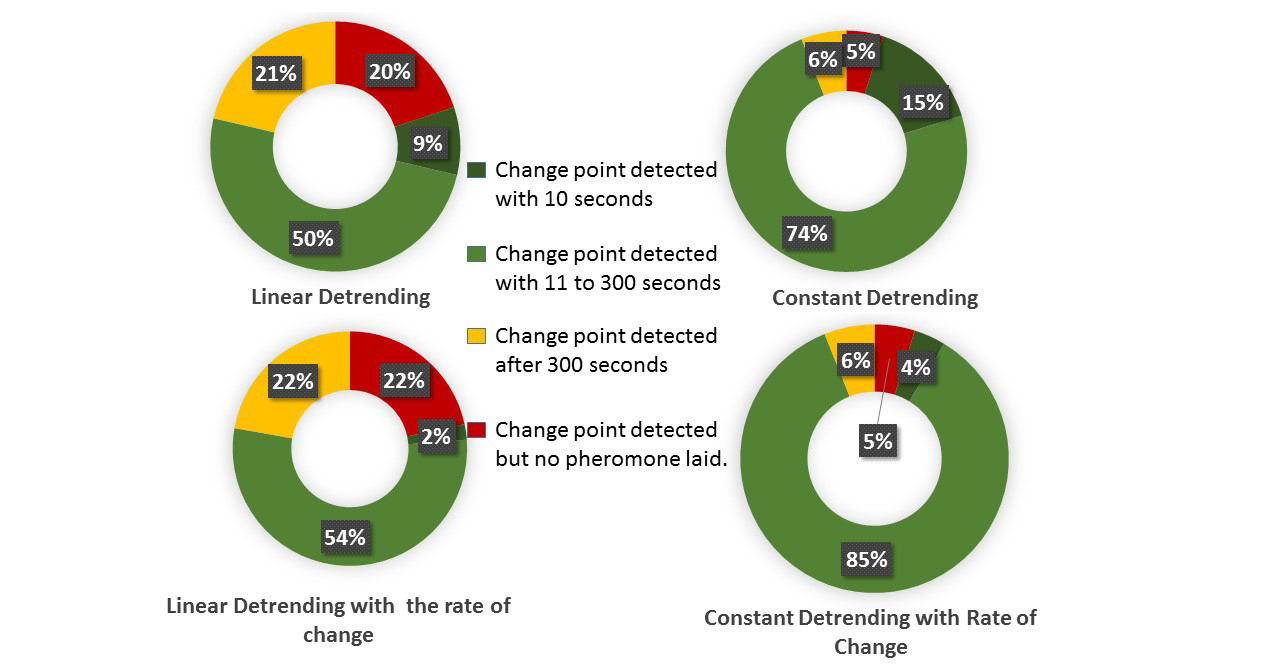
\includegraphics[height=0.35\textheight]{DonutCharts/Slide2.JPG}
	\caption{Efficiency chart for \textit{P. rugosus}, one pile,  communication only setting.}
\end{figure}
\begin{figure}[h]
	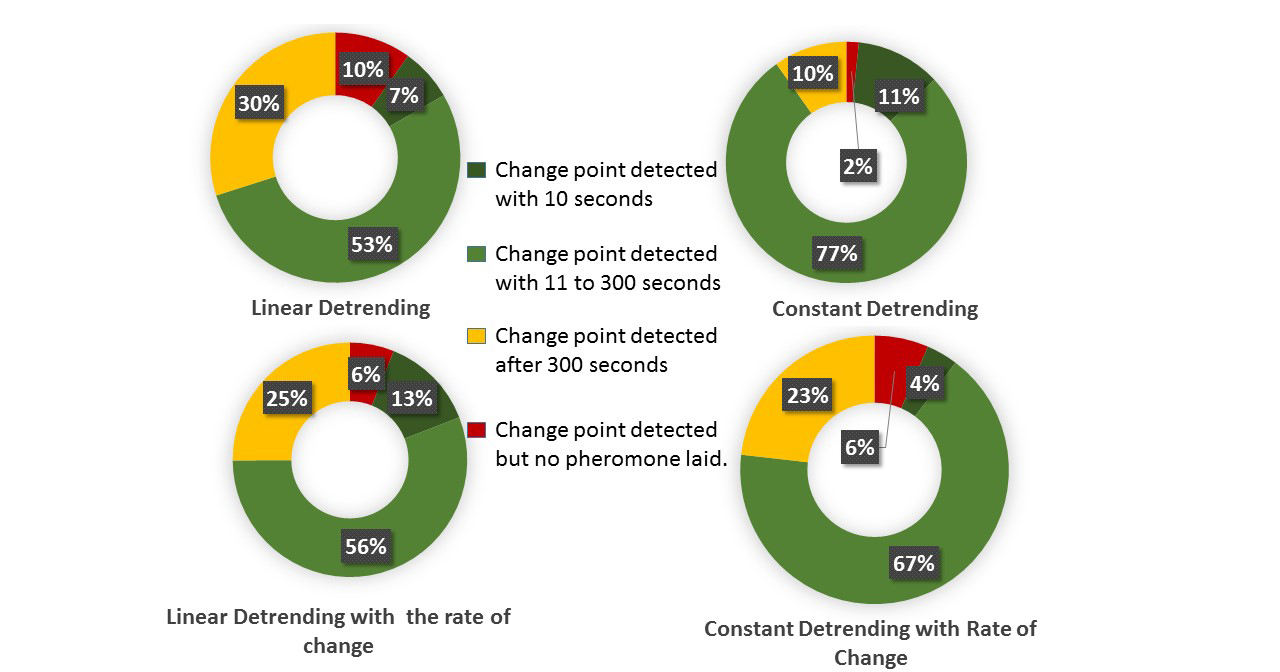
\includegraphics[height=0.35\textheight]{DonutCharts/Slide3.JPG}
\caption{Efficiency chart for \textit{P. rugosus}, four pile,  communication only setting.}
\end{figure}
\begin{figure}[h]
	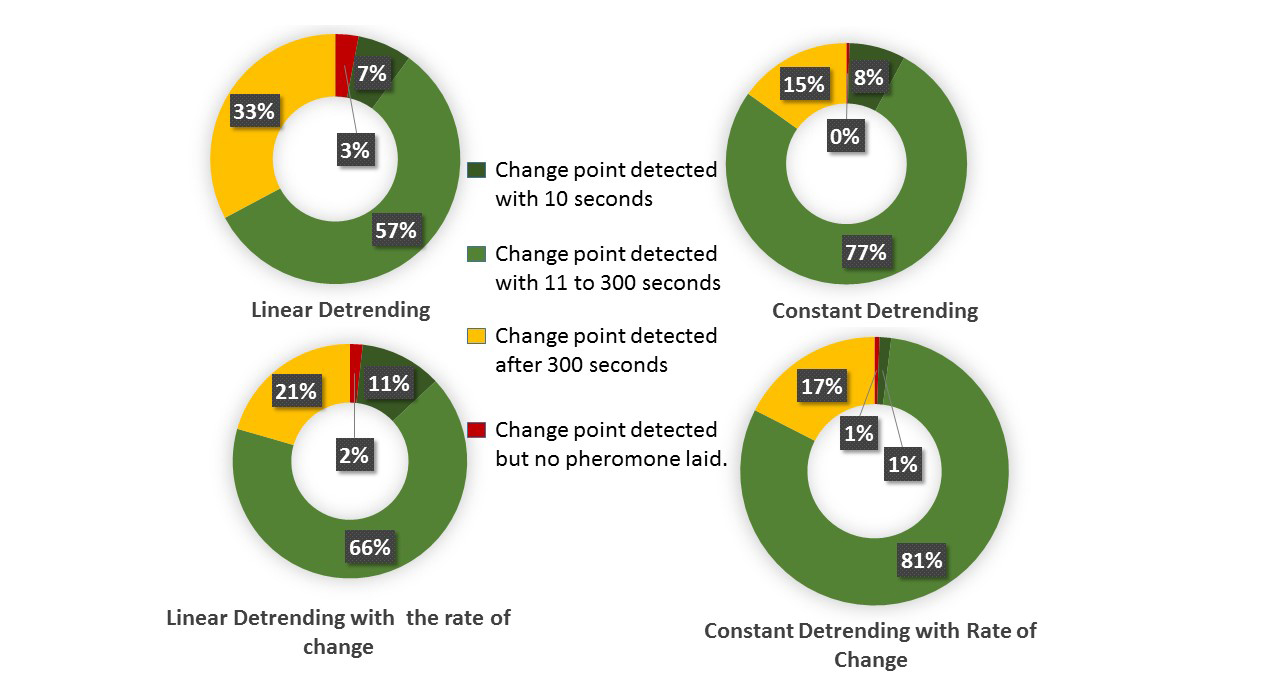
\includegraphics[height=0.35\textheight]{DonutCharts/Slide4.JPG}
	\caption{Efficiency chart for \textit{P. rugosus}, sixteen pile,  communication only setting.}
\end{figure}
\begin{figure}[h]
	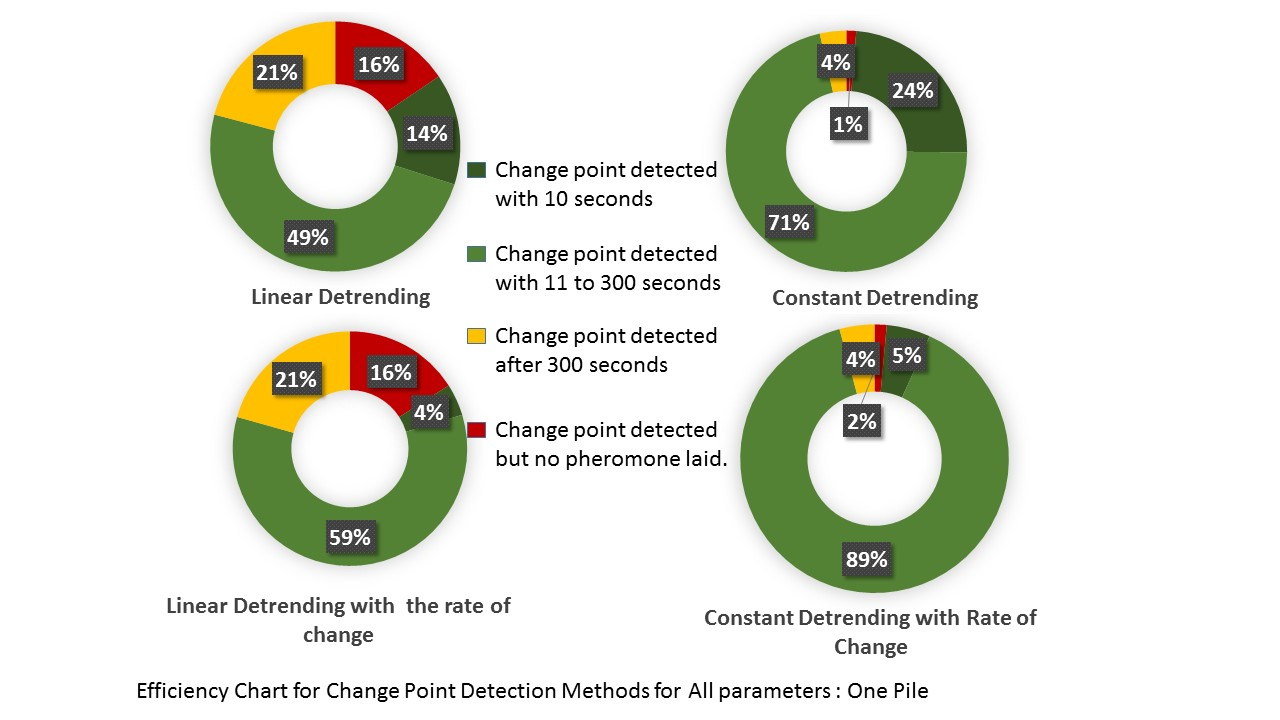
\includegraphics[height=0.35\textheight]{DonutCharts/Slide5.JPG}
	\caption{Efficiency chart for \textit{P. rugosus}, one pile,  memory and communication combined setting.}
\end{figure}
\begin{figure}[h]
	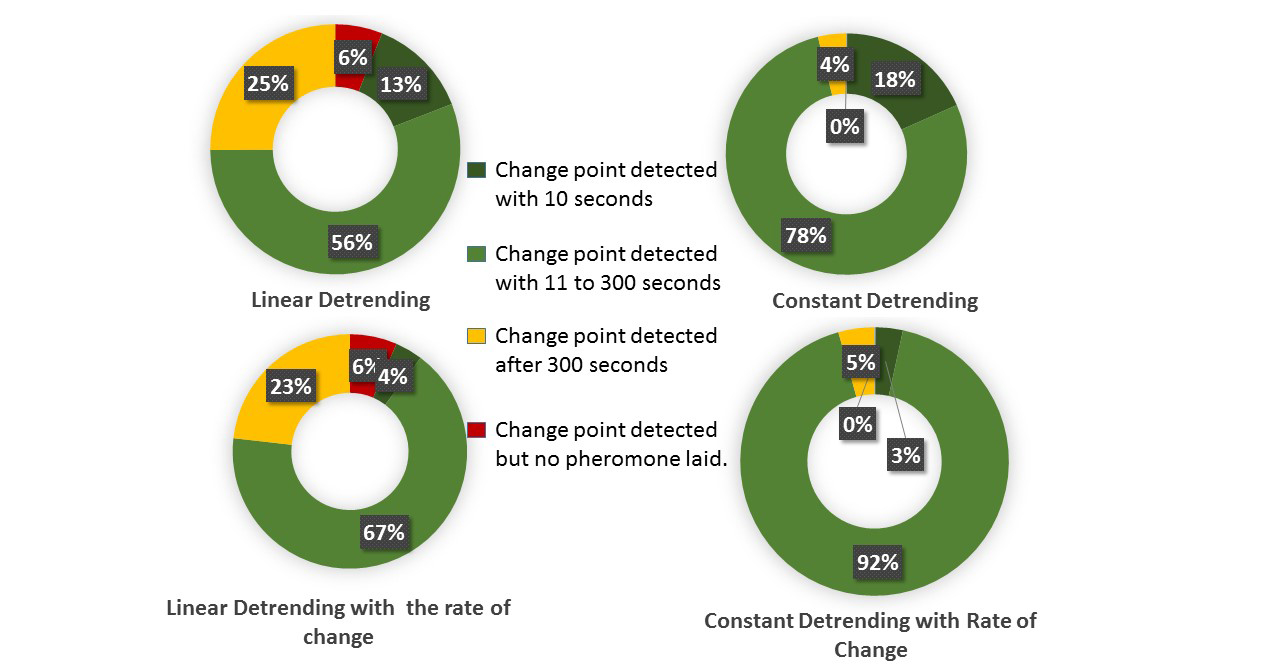
\includegraphics[height=0.35\textheight]{DonutCharts/Slide6.JPG}
	\caption{Efficiency chart for \textit{P. rugosus}, four pile, memory and communication combined setting.}
\end{figure}
\begin{figure}[h]
	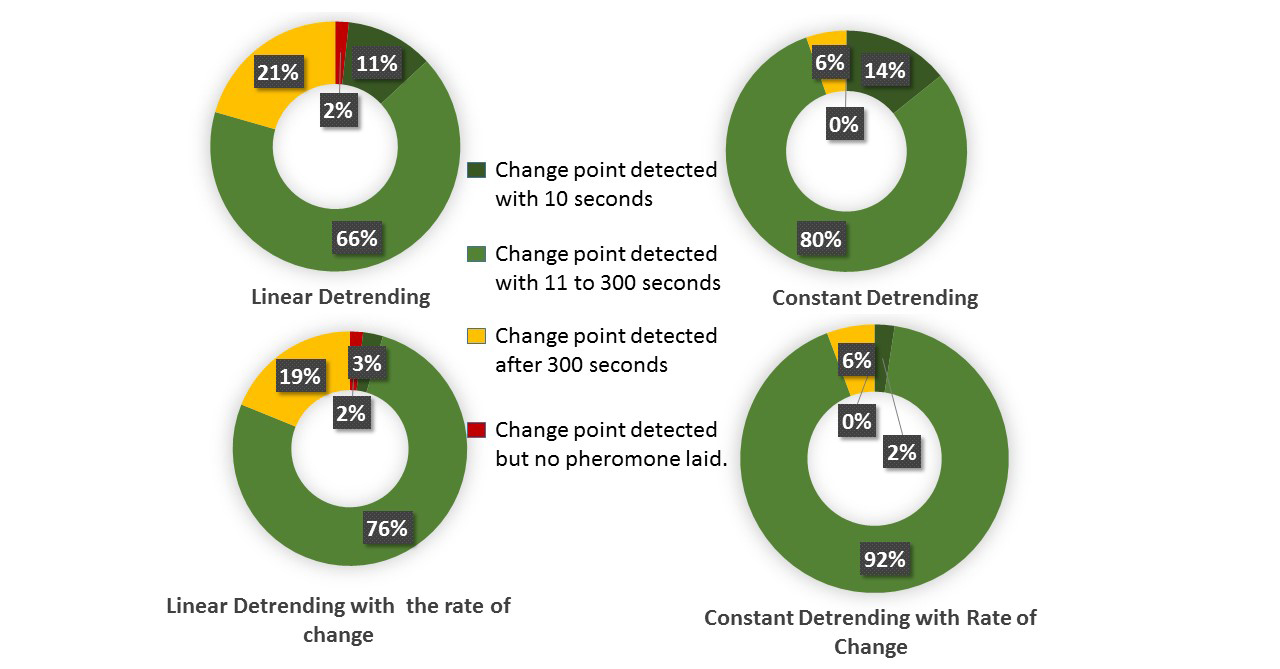
\includegraphics[height=0.35\textheight]{DonutCharts/Slide7.JPG}
	\caption{Efficiency chart for \textit{P. rugosus}, sixteen pile,  memory and communication combined setting.}
\end{figure}
\begin{figure}[h]
	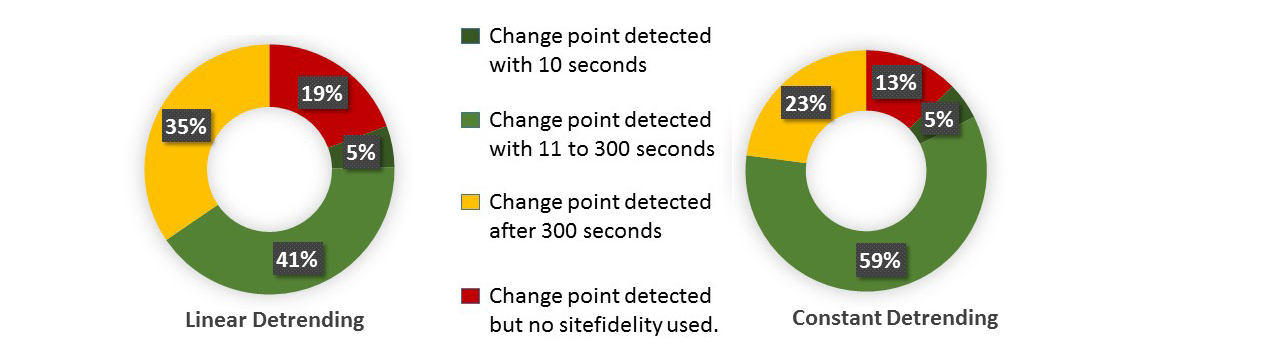
\includegraphics[width=\textwidth]{DonutCharts/Slide8.JPG}
	\caption{Efficiency chart for \textit{P. rugosus}, one pile,  memory only setting.}
\end{figure}
\begin{figure}[h]
	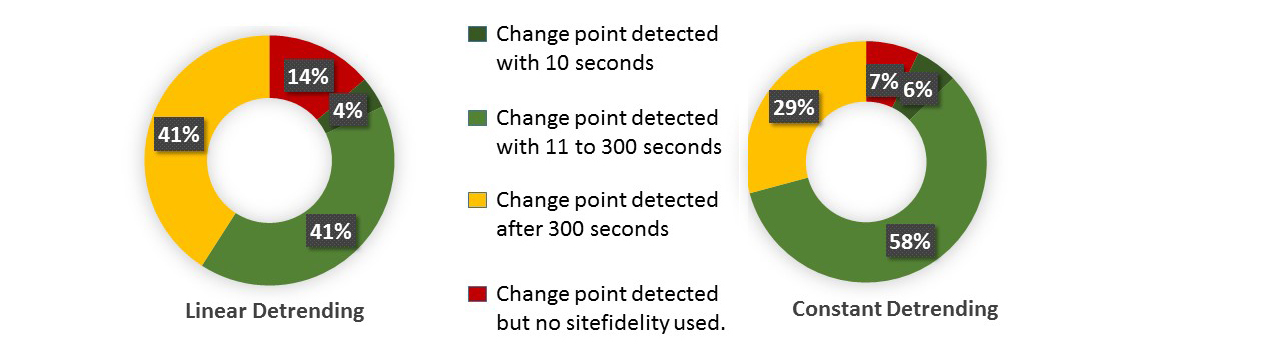
\includegraphics[width=\textwidth]{DonutCharts/Slide9.JPG}
	\caption{Efficiency chart for \textit{P. rugosus}, four pile,  memory only setting.}
\end{figure}
\begin{figure}[h]
	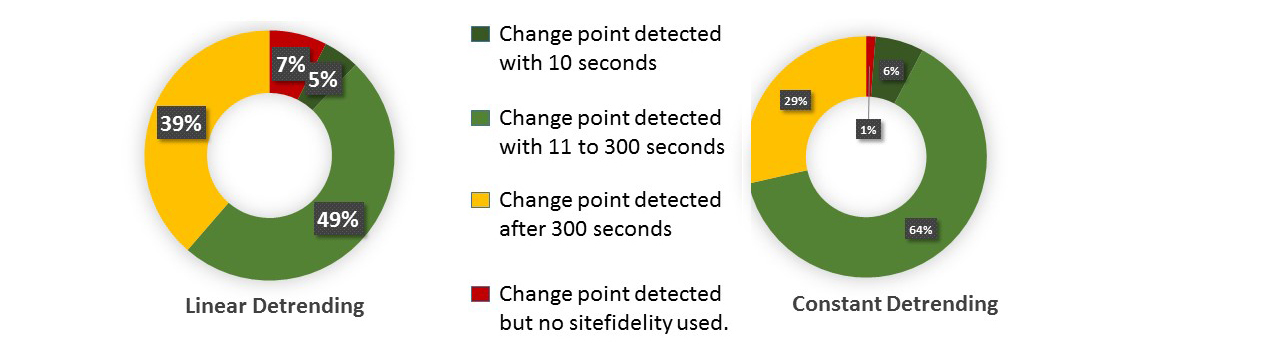
\includegraphics[width=\textwidth]{DonutCharts/Slide10.JPG}
	\caption{Efficiency chart for \textit{P. rugosus}, sixteen pile,  memory only setting.}
\end{figure}
\begin{figure}[h]
	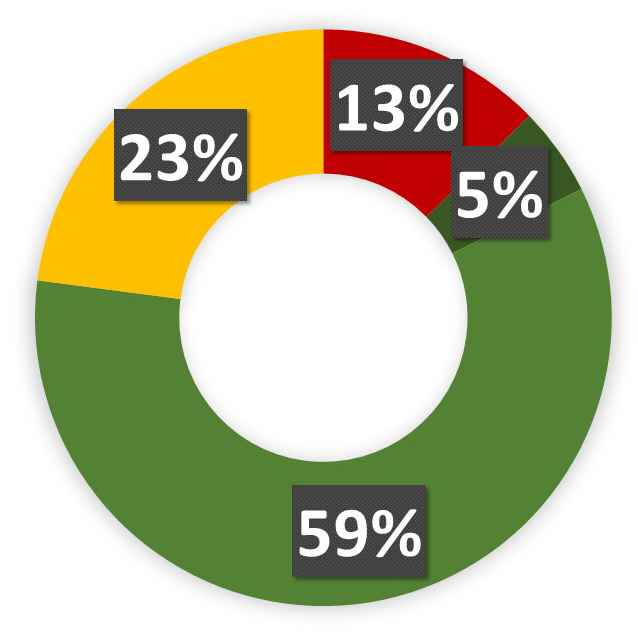
\includegraphics[height=0.35\textheight]{DesertorumDonutCharts/Slide12.JPG}
	\caption{Efficiency chart for \textit{P. desertorum}, one pile,  communication only setting.}
\end{figure}
\begin{figure}[h]
	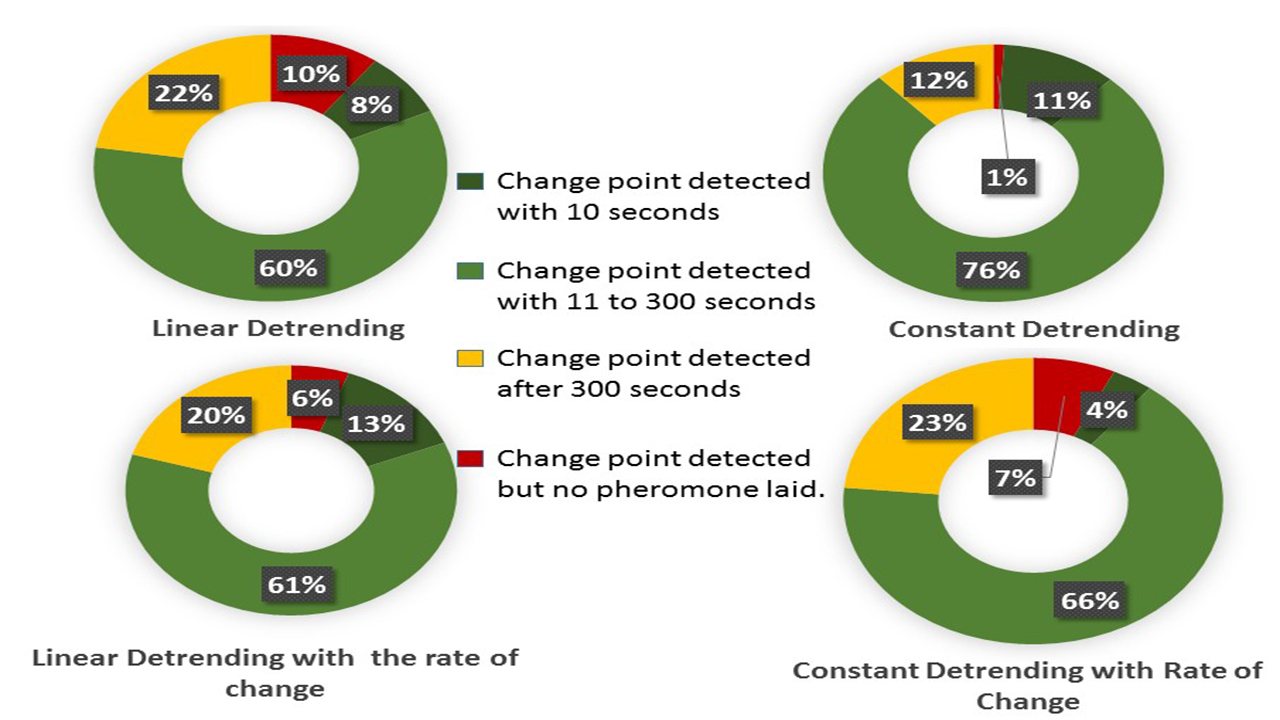
\includegraphics[height=0.35\textheight]{DesertorumDonutCharts/Slide13.JPG}
	\caption{Efficiency chart for \textit{P. desertorum}, four pile,  communication only setting.}
\end{figure}
\begin{figure}[h]
	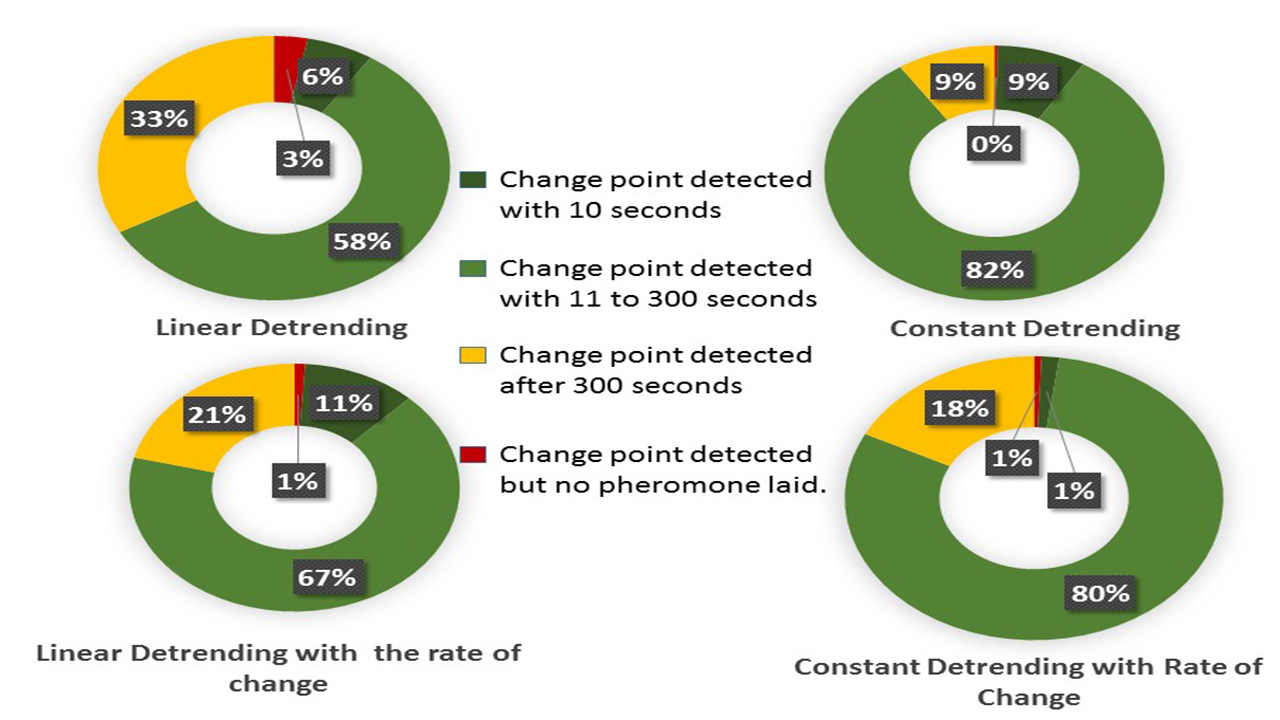
\includegraphics[height=0.35\textheight]{DesertorumDonutCharts/Slide14.JPG}
	\caption{Efficiency chart for \textit{P. desertorum}, sixteen pile,  communication only setting.}
\end{figure}
\begin{figure}[h]
	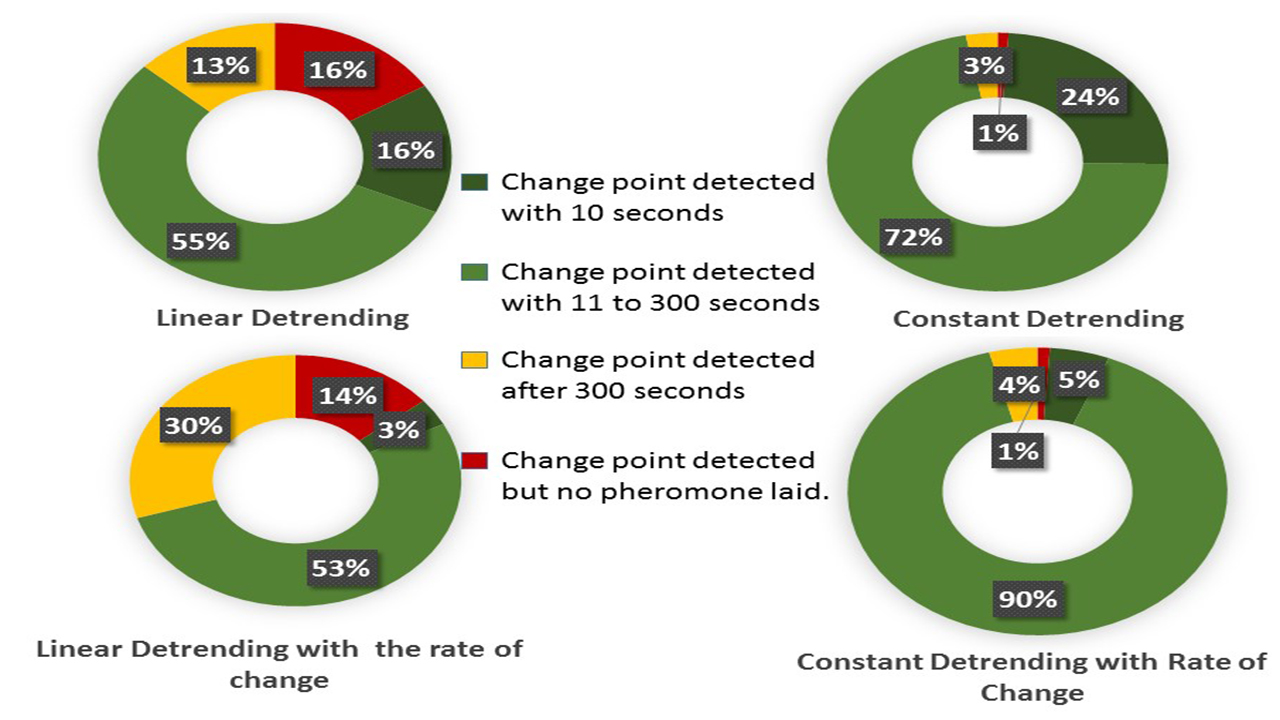
\includegraphics[height=0.35\textheight]{DesertorumDonutCharts/Slide15.JPG}
	\caption{Efficiency chart for \textit{P. desertorum}, one pile,  memory and communication combined setting.}
\end{figure}
\begin{figure}[h]
	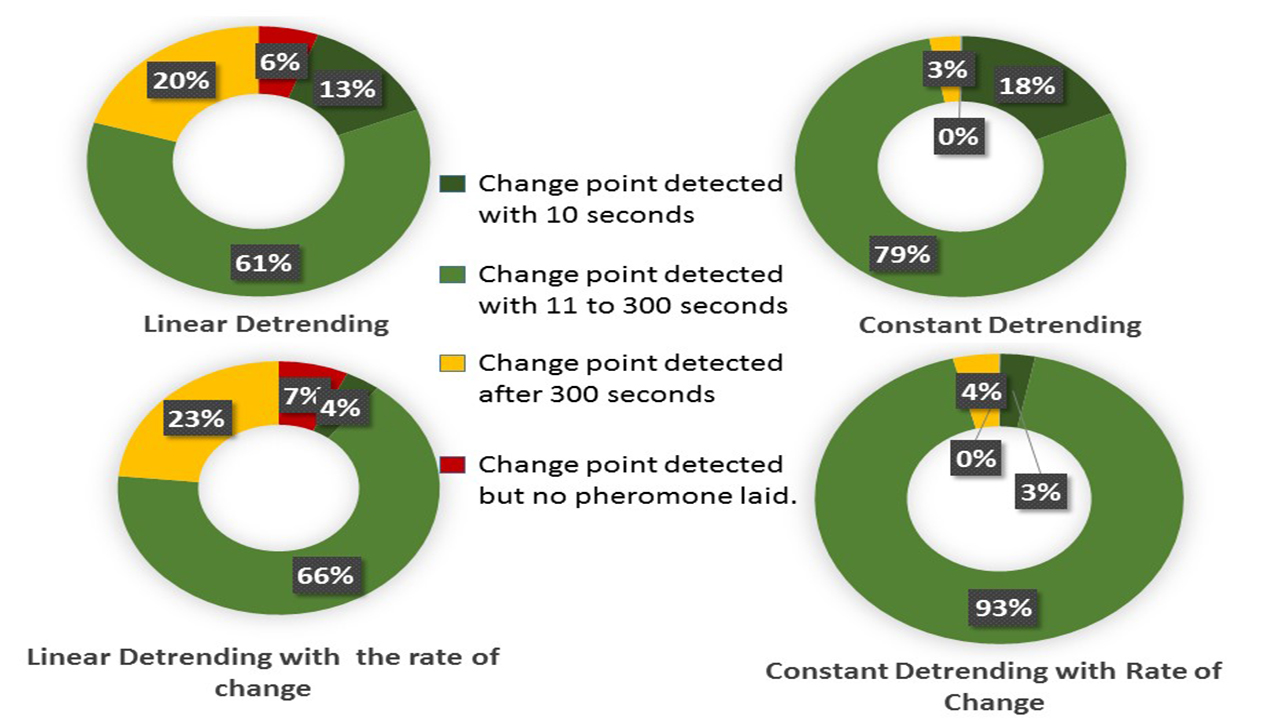
\includegraphics[height=0.35\textheight]{DesertorumDonutCharts/Slide16.JPG}
	\caption{Efficiency chart for \textit{P. desertorum}, four pile, memory and communication combined setting.}
\end{figure}
\begin{figure}[h]
	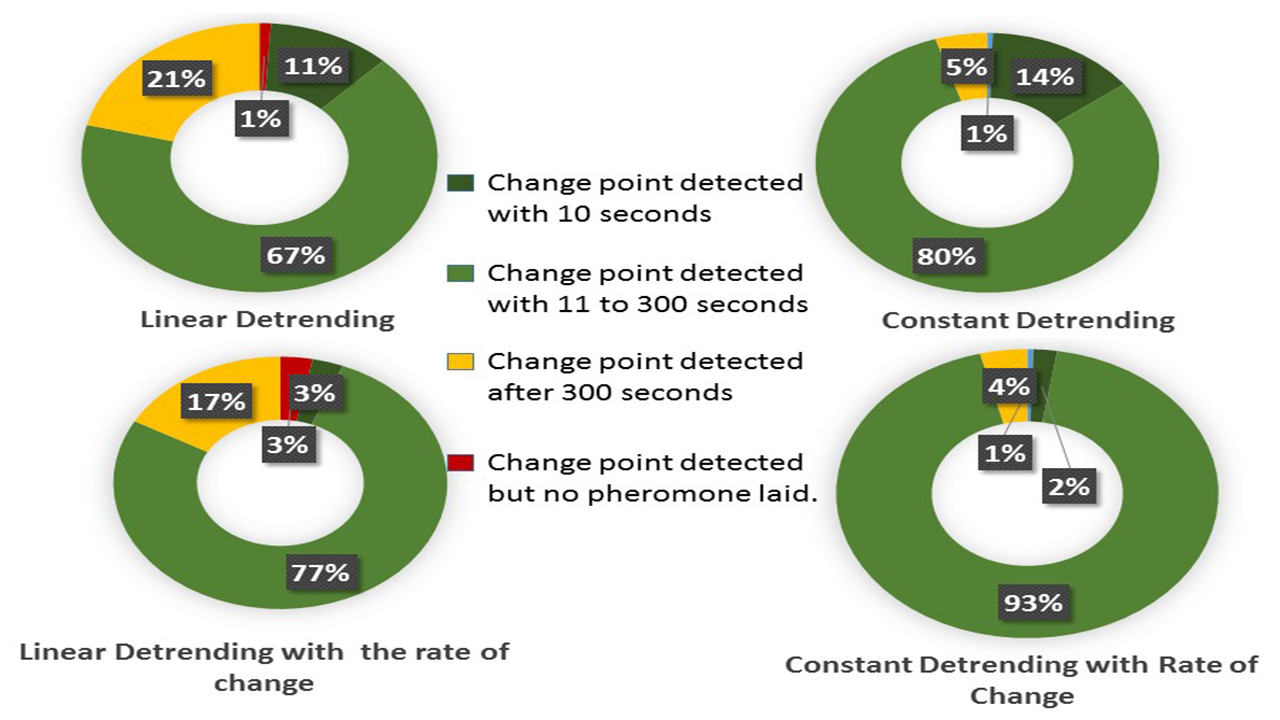
\includegraphics[height=0.35\textheight]{DesertorumDonutCharts/Slide17.JPG}
	\caption{Efficiency chart for \textit{P. desertorum}, sixteen pile,  memory and communication combined setting.}
\end{figure}
\begin{figure}[h]
	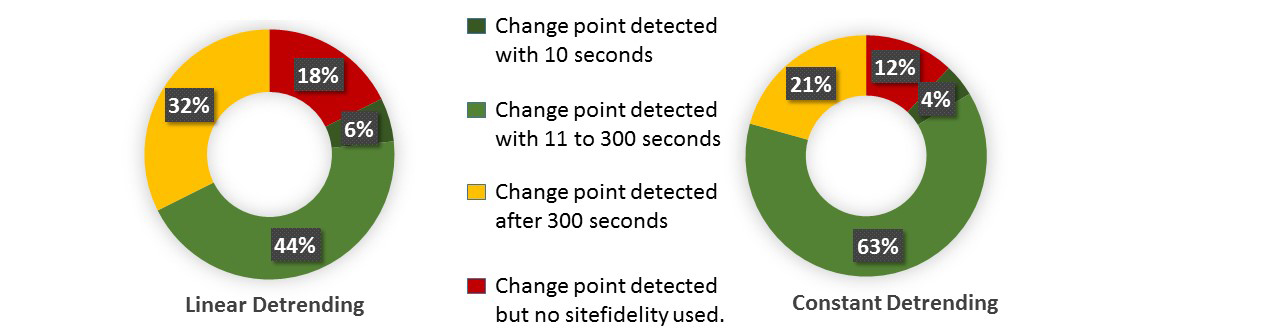
\includegraphics[width=\textwidth]{DesertorumDonutCharts/Slide18.JPG}
	\caption{Efficiency chart for \textit{P. desertorum}, one pile,  memory only setting.}
\end{figure}
\begin{figure}[h]
	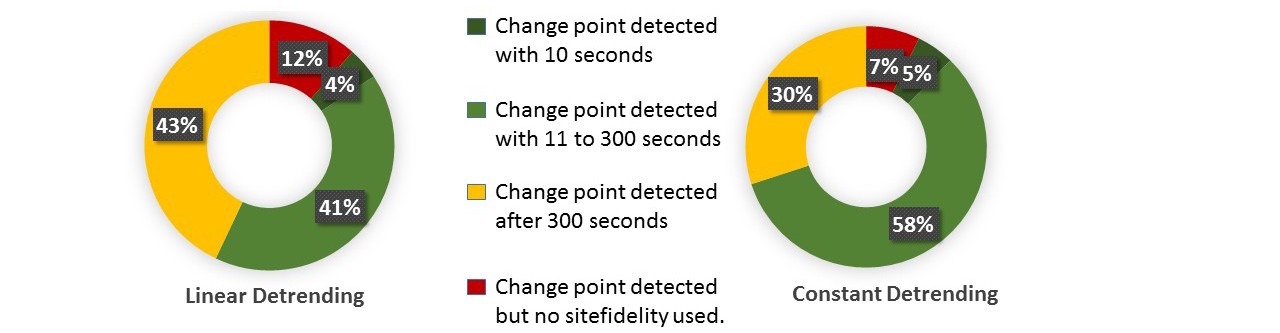
\includegraphics[width=\textwidth]{DesertorumDonutCharts/Slide19.JPG}
	\caption{Efficiency chart for \textit{P. desertorum}, four pile,  memory only setting.}
\end{figure}
\clearpage
\begin{figure}[h]
	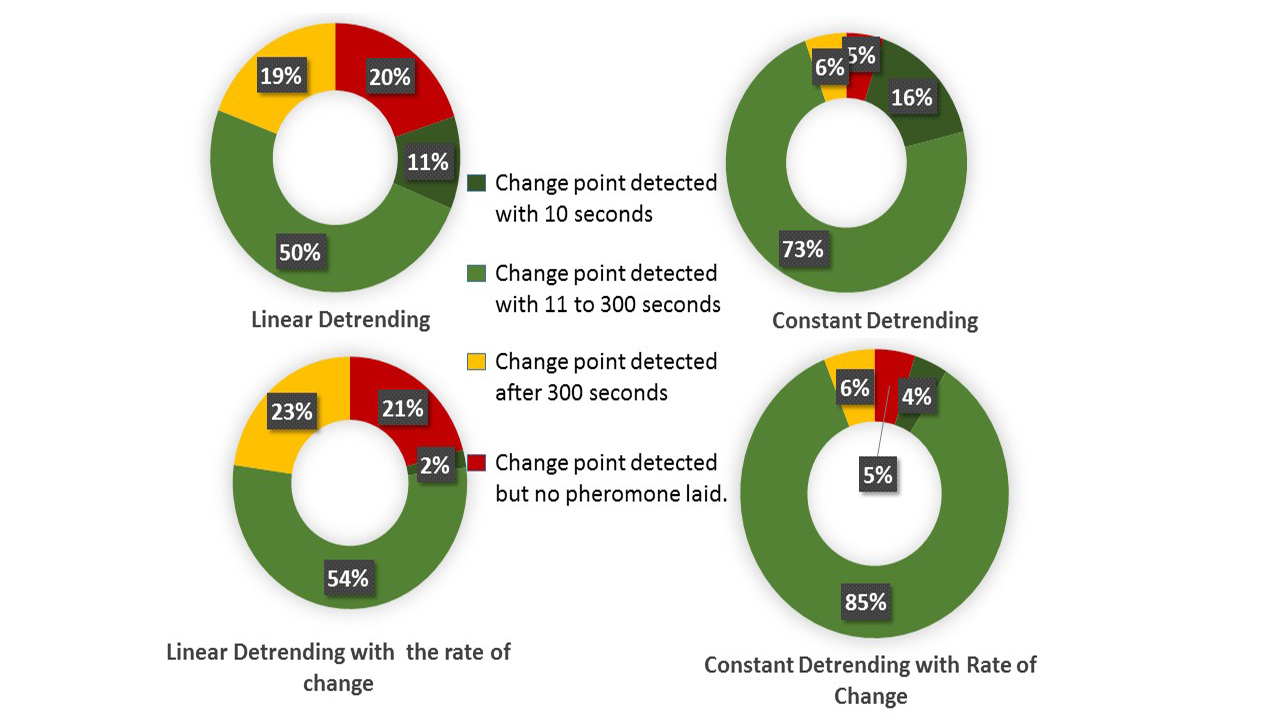
\includegraphics[height=0.35\textheight]{MaricopaDonutCharts/Slide22.JPG}
	\caption{Efficiency chart for \textit{P. maricopa}, one pile,  communication only setting.}
\end{figure}
\begin{figure}[h]
	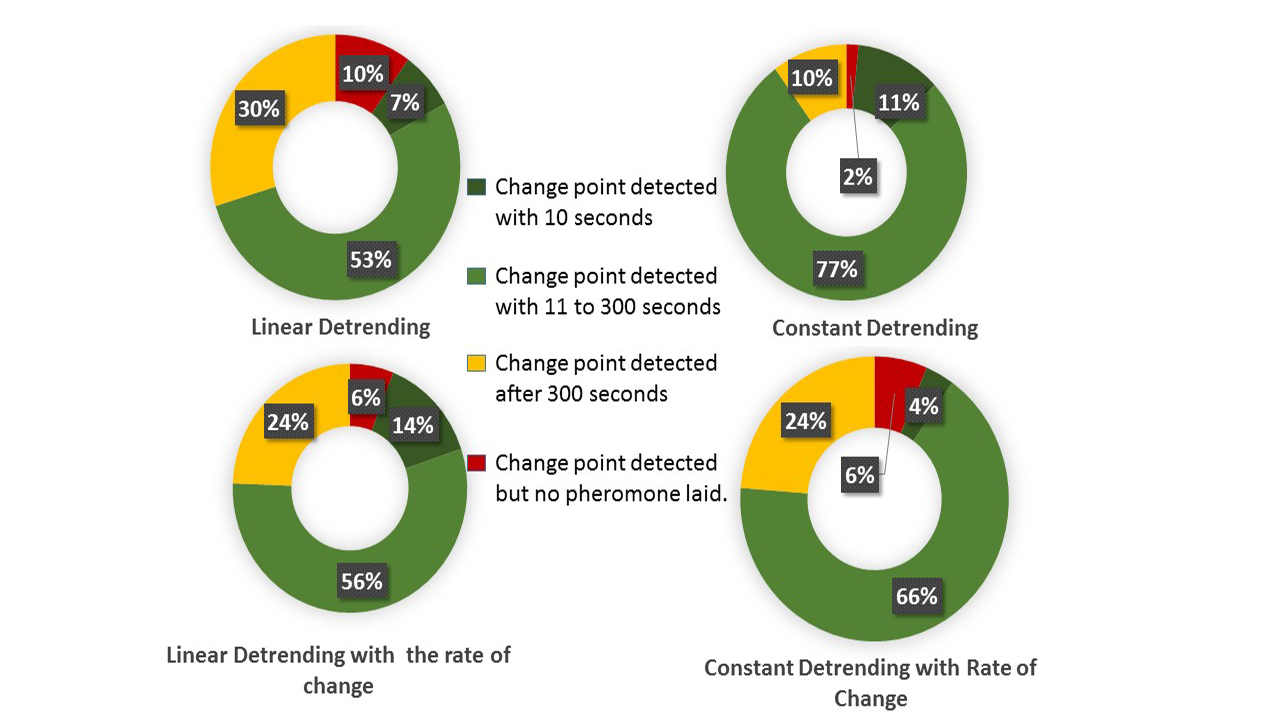
\includegraphics[height=0.35\textheight]{MaricopaDonutCharts/Slide23.JPG}
	\caption{Efficiency chart for \textit{P. maricopa}, four pile,  communication only setting.}
\end{figure}
\begin{figure}[h]
	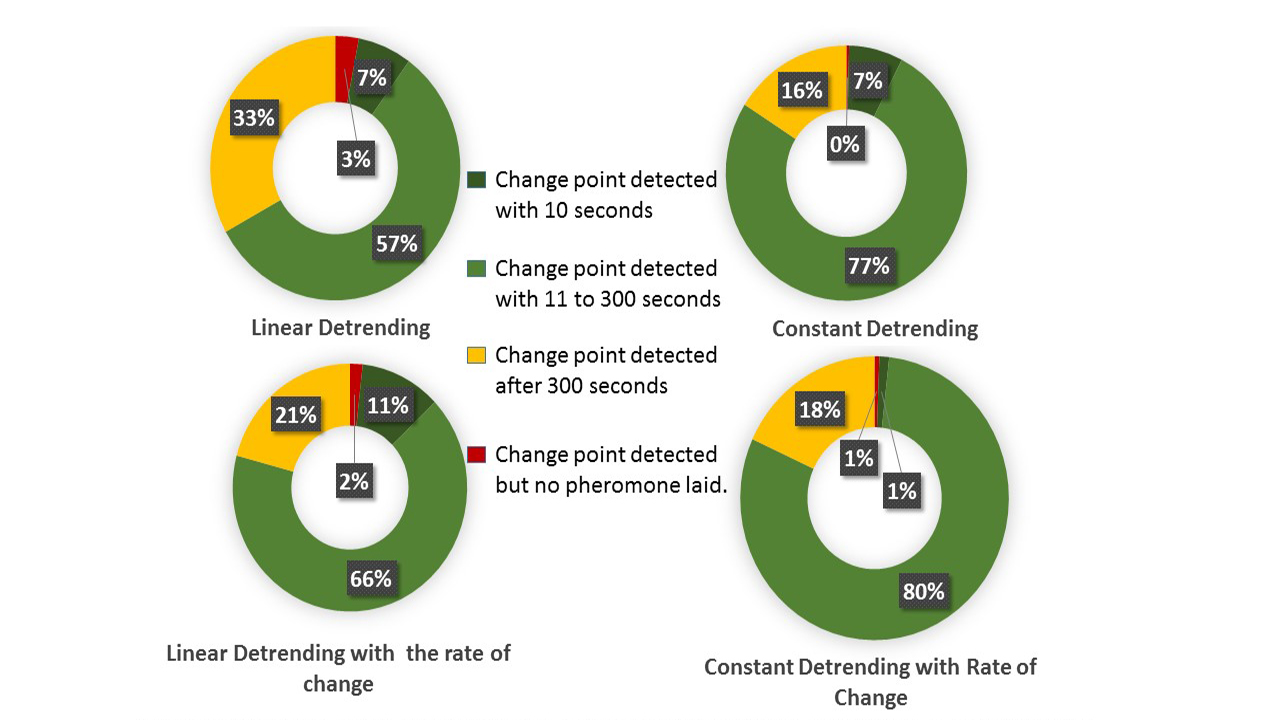
\includegraphics[height=0.35\textheight]{MaricopaDonutCharts/Slide24.JPG}
	\caption{Efficiency chart for \textit{P. maricopa}, sixteen pile,  communication only setting.}
\end{figure}
\begin{figure}[h]
	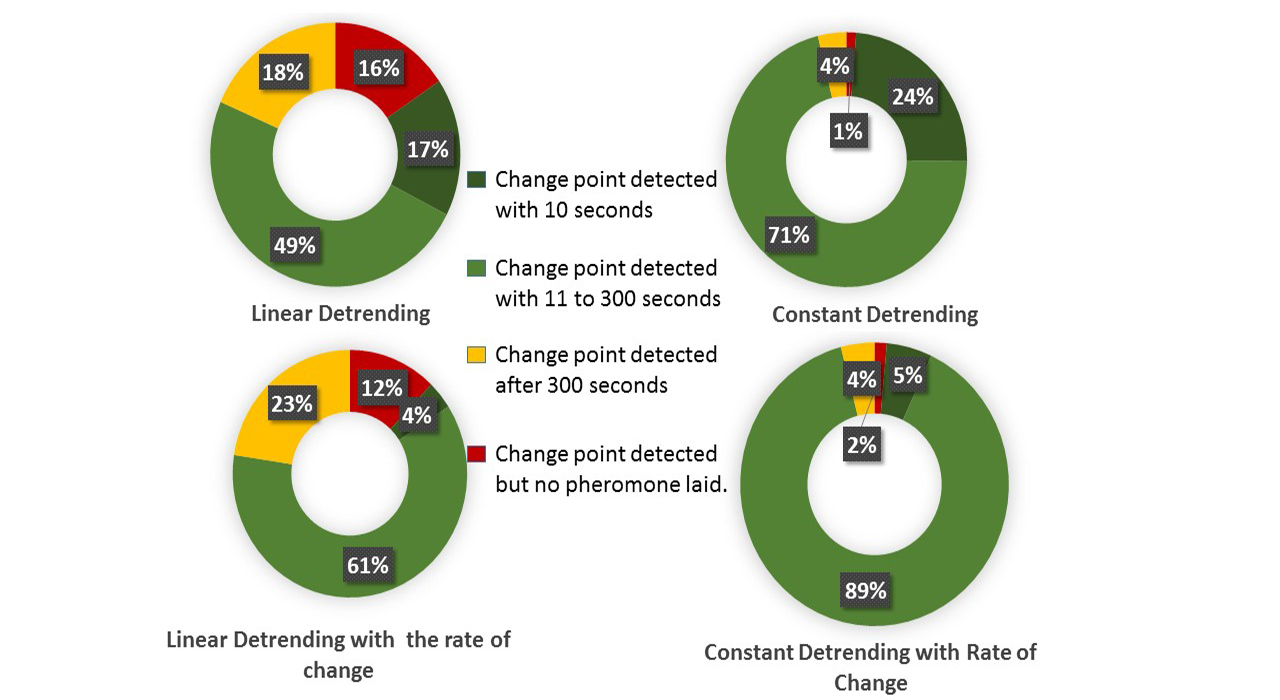
\includegraphics[height=0.35\textheight]{MaricopaDonutCharts/Slide25.JPG}
	\caption{Efficiency chart for \textit{P. maricopa}, one pile,  memory and communication combined setting.}
\end{figure}
\begin{figure}[h]
	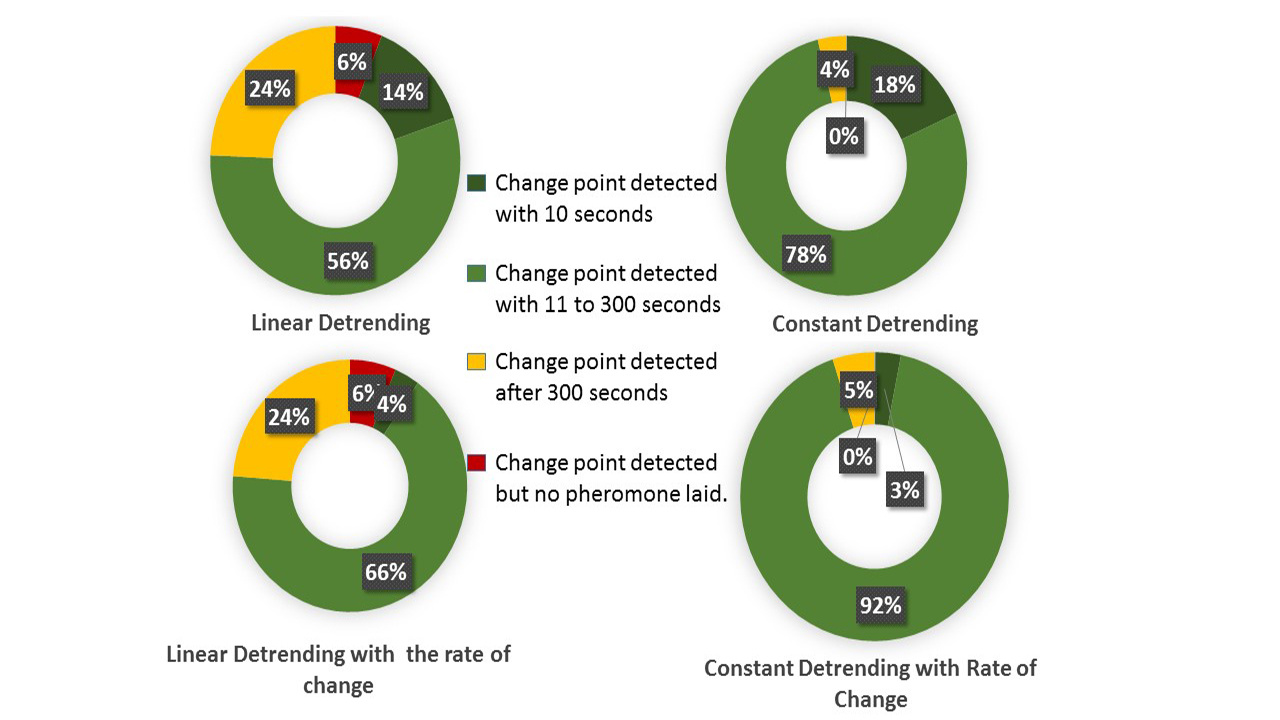
\includegraphics[height=0.35\textheight]{MaricopaDonutCharts/Slide26.JPG}
	\caption{Efficiency chart for \textit{P. maricopa}, four pile, memory and communication combined setting.}
\end{figure}
\begin{figure}[h]
	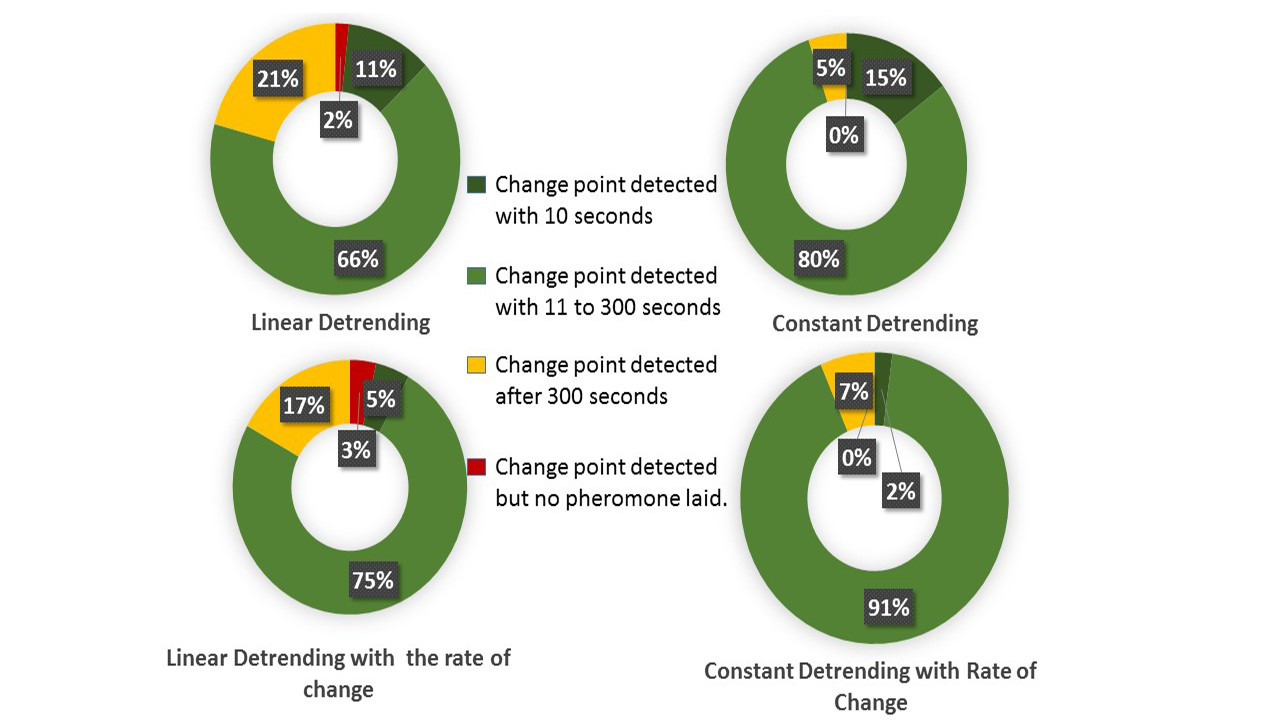
\includegraphics[height=0.35\textheight]{MaricopaDonutCharts/Slide27.JPG}
	\caption{Efficiency chart for \textit{P. maricopa}, sixteen pile,  memory and communication combined setting.}
\end{figure}
\begin{figure}[h]
	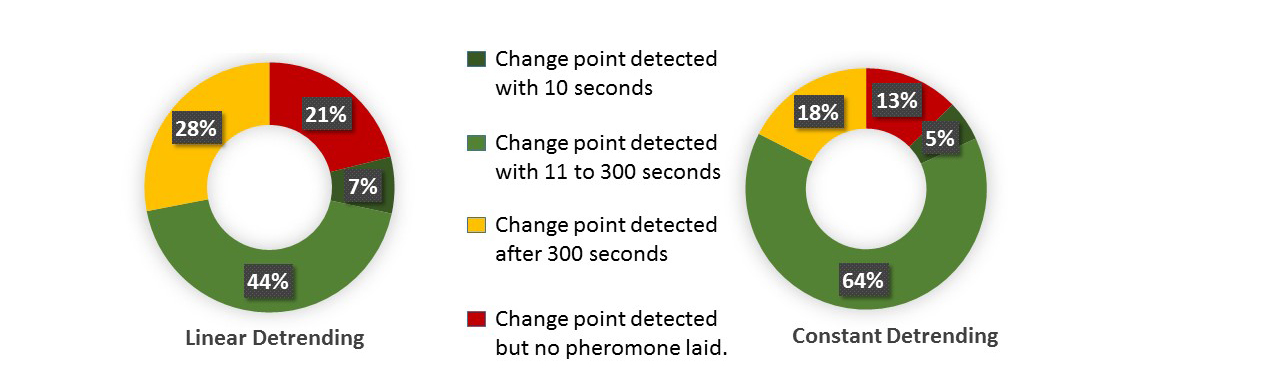
\includegraphics[width=\textwidth]{MaricopaDonutCharts/Slide28.JPG}
	\caption{Efficiency chart for \textit{P. maricopa}, one pile,  memory only setting.}
\end{figure}
\begin{figure}[h]
	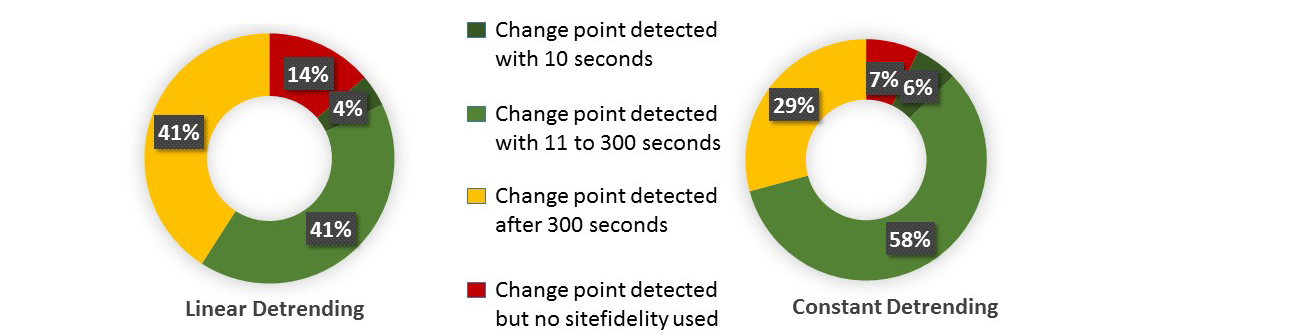
\includegraphics[width=\textwidth]{MaricopaDonutCharts/Slide29.JPG}
	\caption{Efficiency chart for \textit{P. maricopa}, four pile,  memory only setting.}
\end{figure}
\begin{figure}[h]
	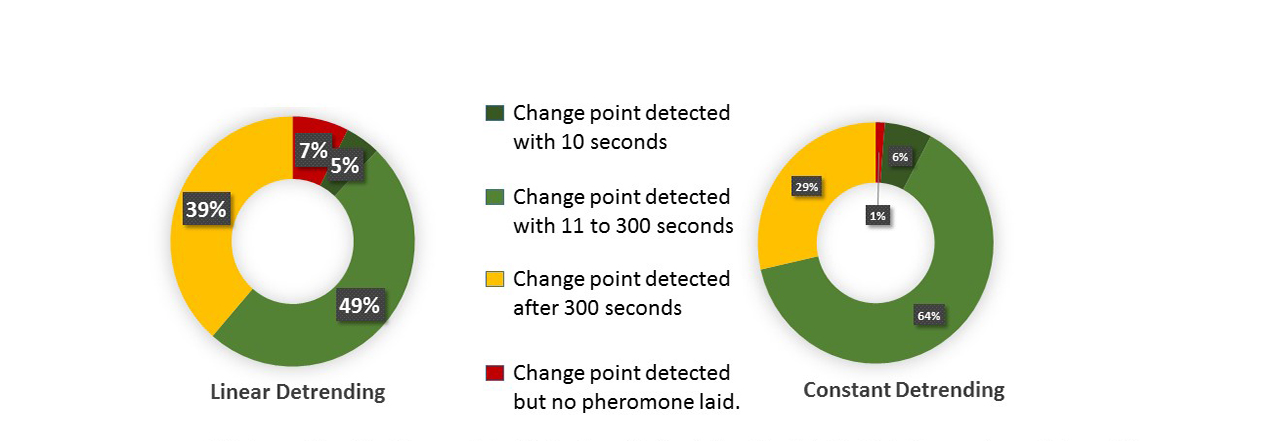
\includegraphics[width=\textwidth]{MaricopaDonutCharts/Slide30.JPG}
	\caption{Efficiency chart for \textit{P. maricopa}, sixteen pile,  memory only setting.}
\end{figure}
\clearpage
\begin{figure}
	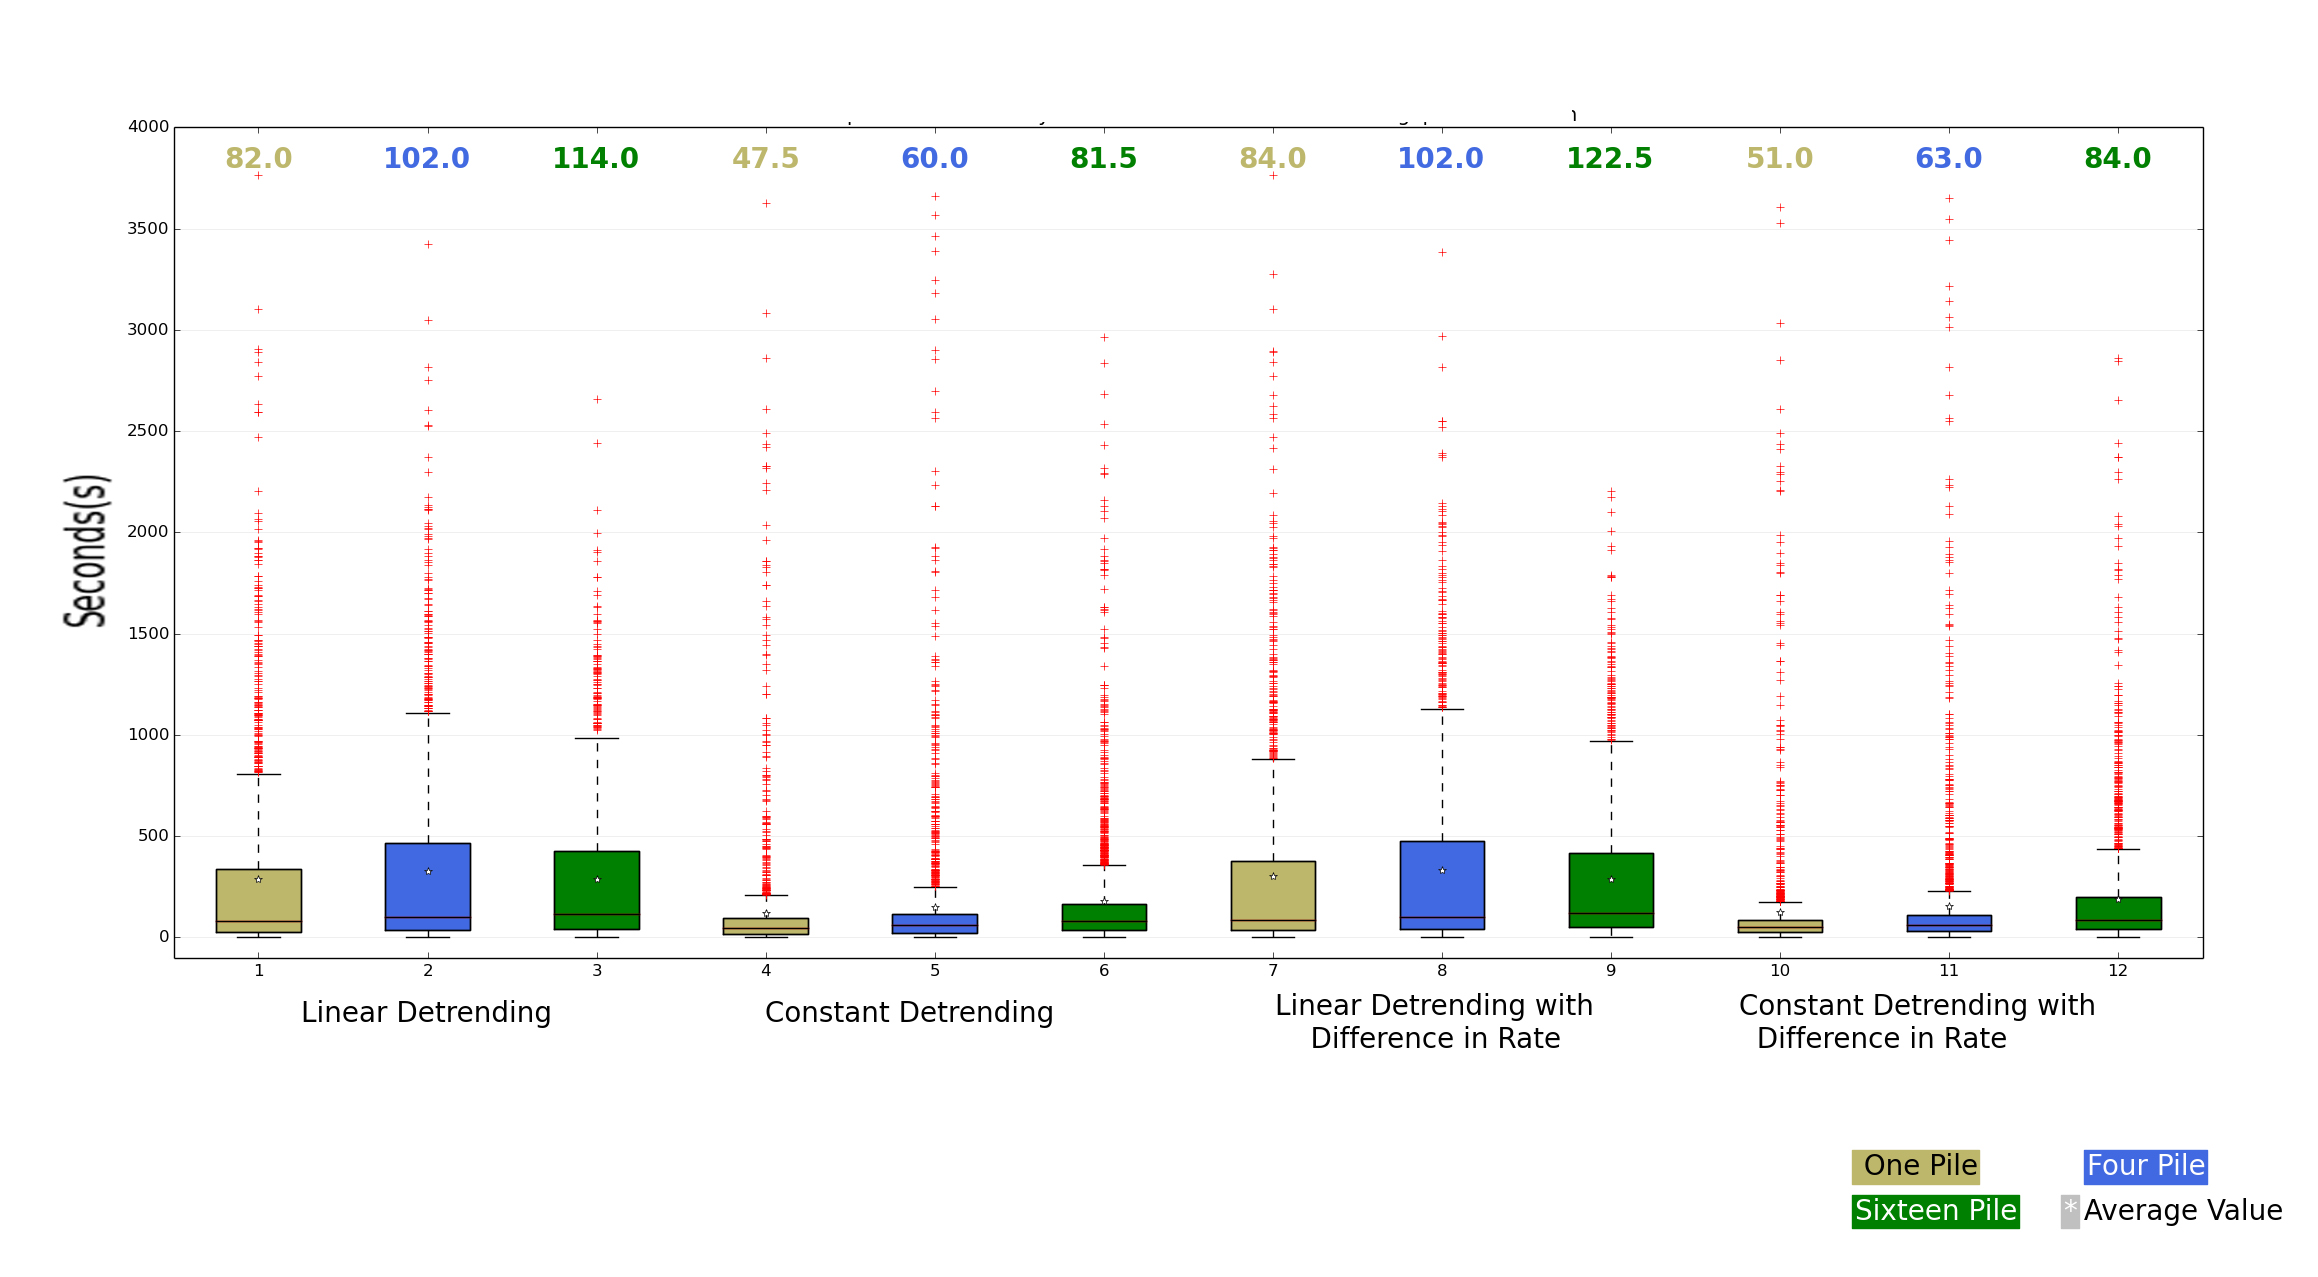
\includegraphics[width=\textwidth,height=0.35\textheight]{PheromoneOnly/PheromoneOnly.jpg}
	\caption{Comparison of change point detection methods for pheromone only parameters for \textit{P. rugosus}. The time in seconds represents the difference between a pheromone laying event followed by a detection of change point in the foraging rate.}
\end{figure}
\begin{figure}
	\includegraphics[width=\textwidth,height=0.35\textheight]{PheromoneOnly/AllPlot.png}
	\caption{Comparison of change point detection method without outliers for pheromone only parameters \textit{P. rugosus}.The time in seconds represents the difference between a pheromone laying event followed by a detection of change point in the foraging rate.}
\end{figure}
\begin{figure}
	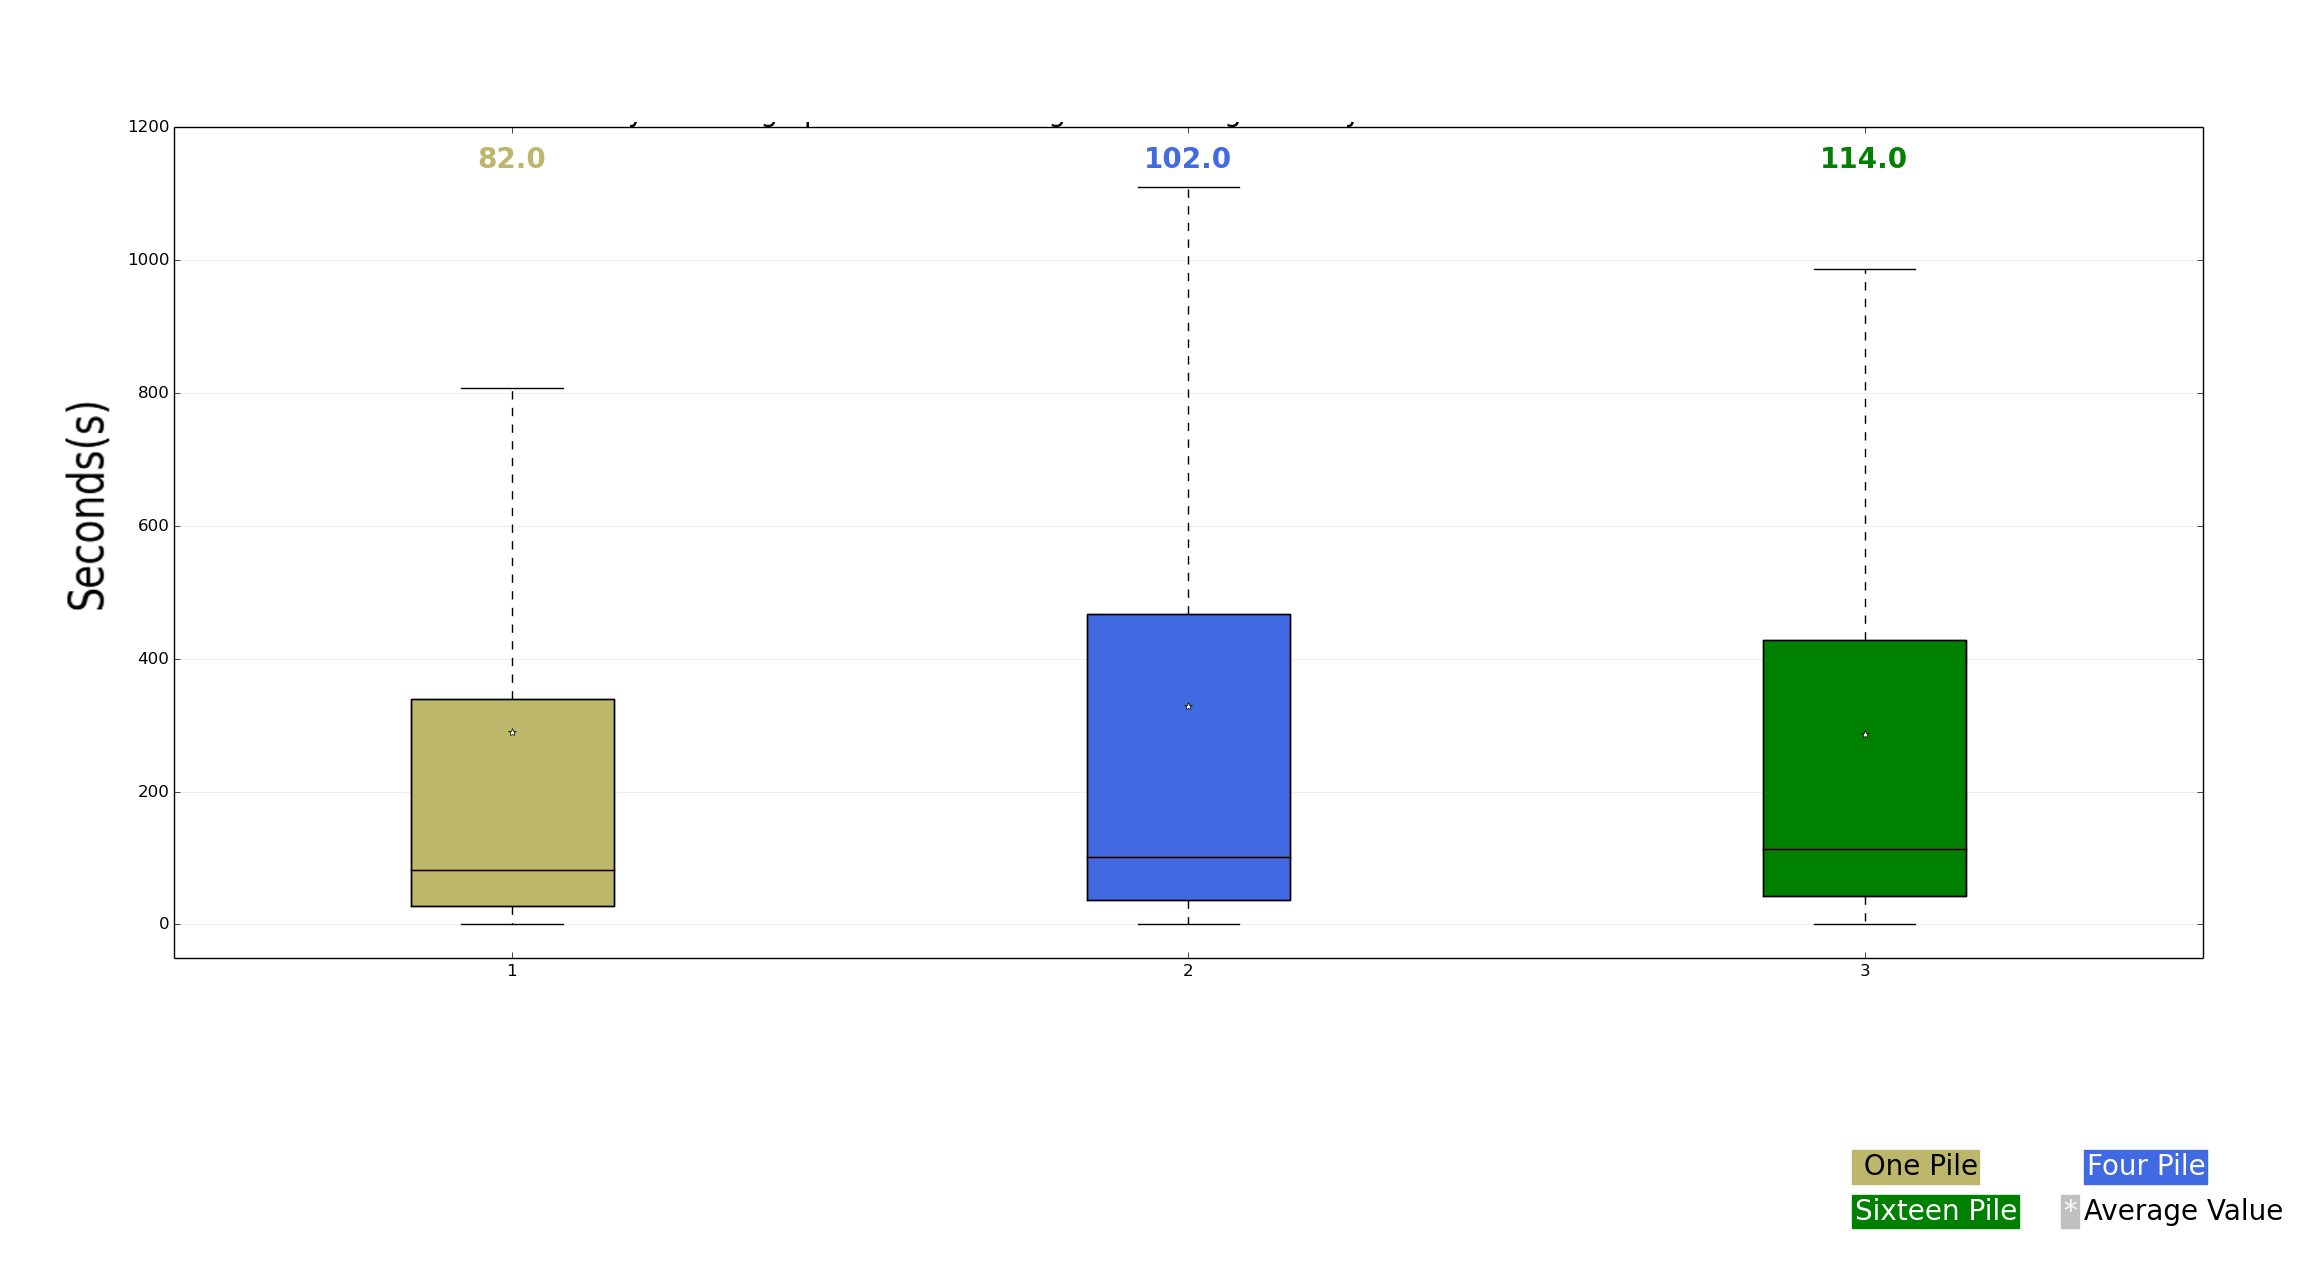
\includegraphics[width=\textwidth,height=0.35\textheight]{PheromoneOnly/Linear.png}
	\caption{Efficiency of Linear Detrending method on data of \textit{P. rugosus} for pheromone only settings}
\end{figure}
\begin{figure}
	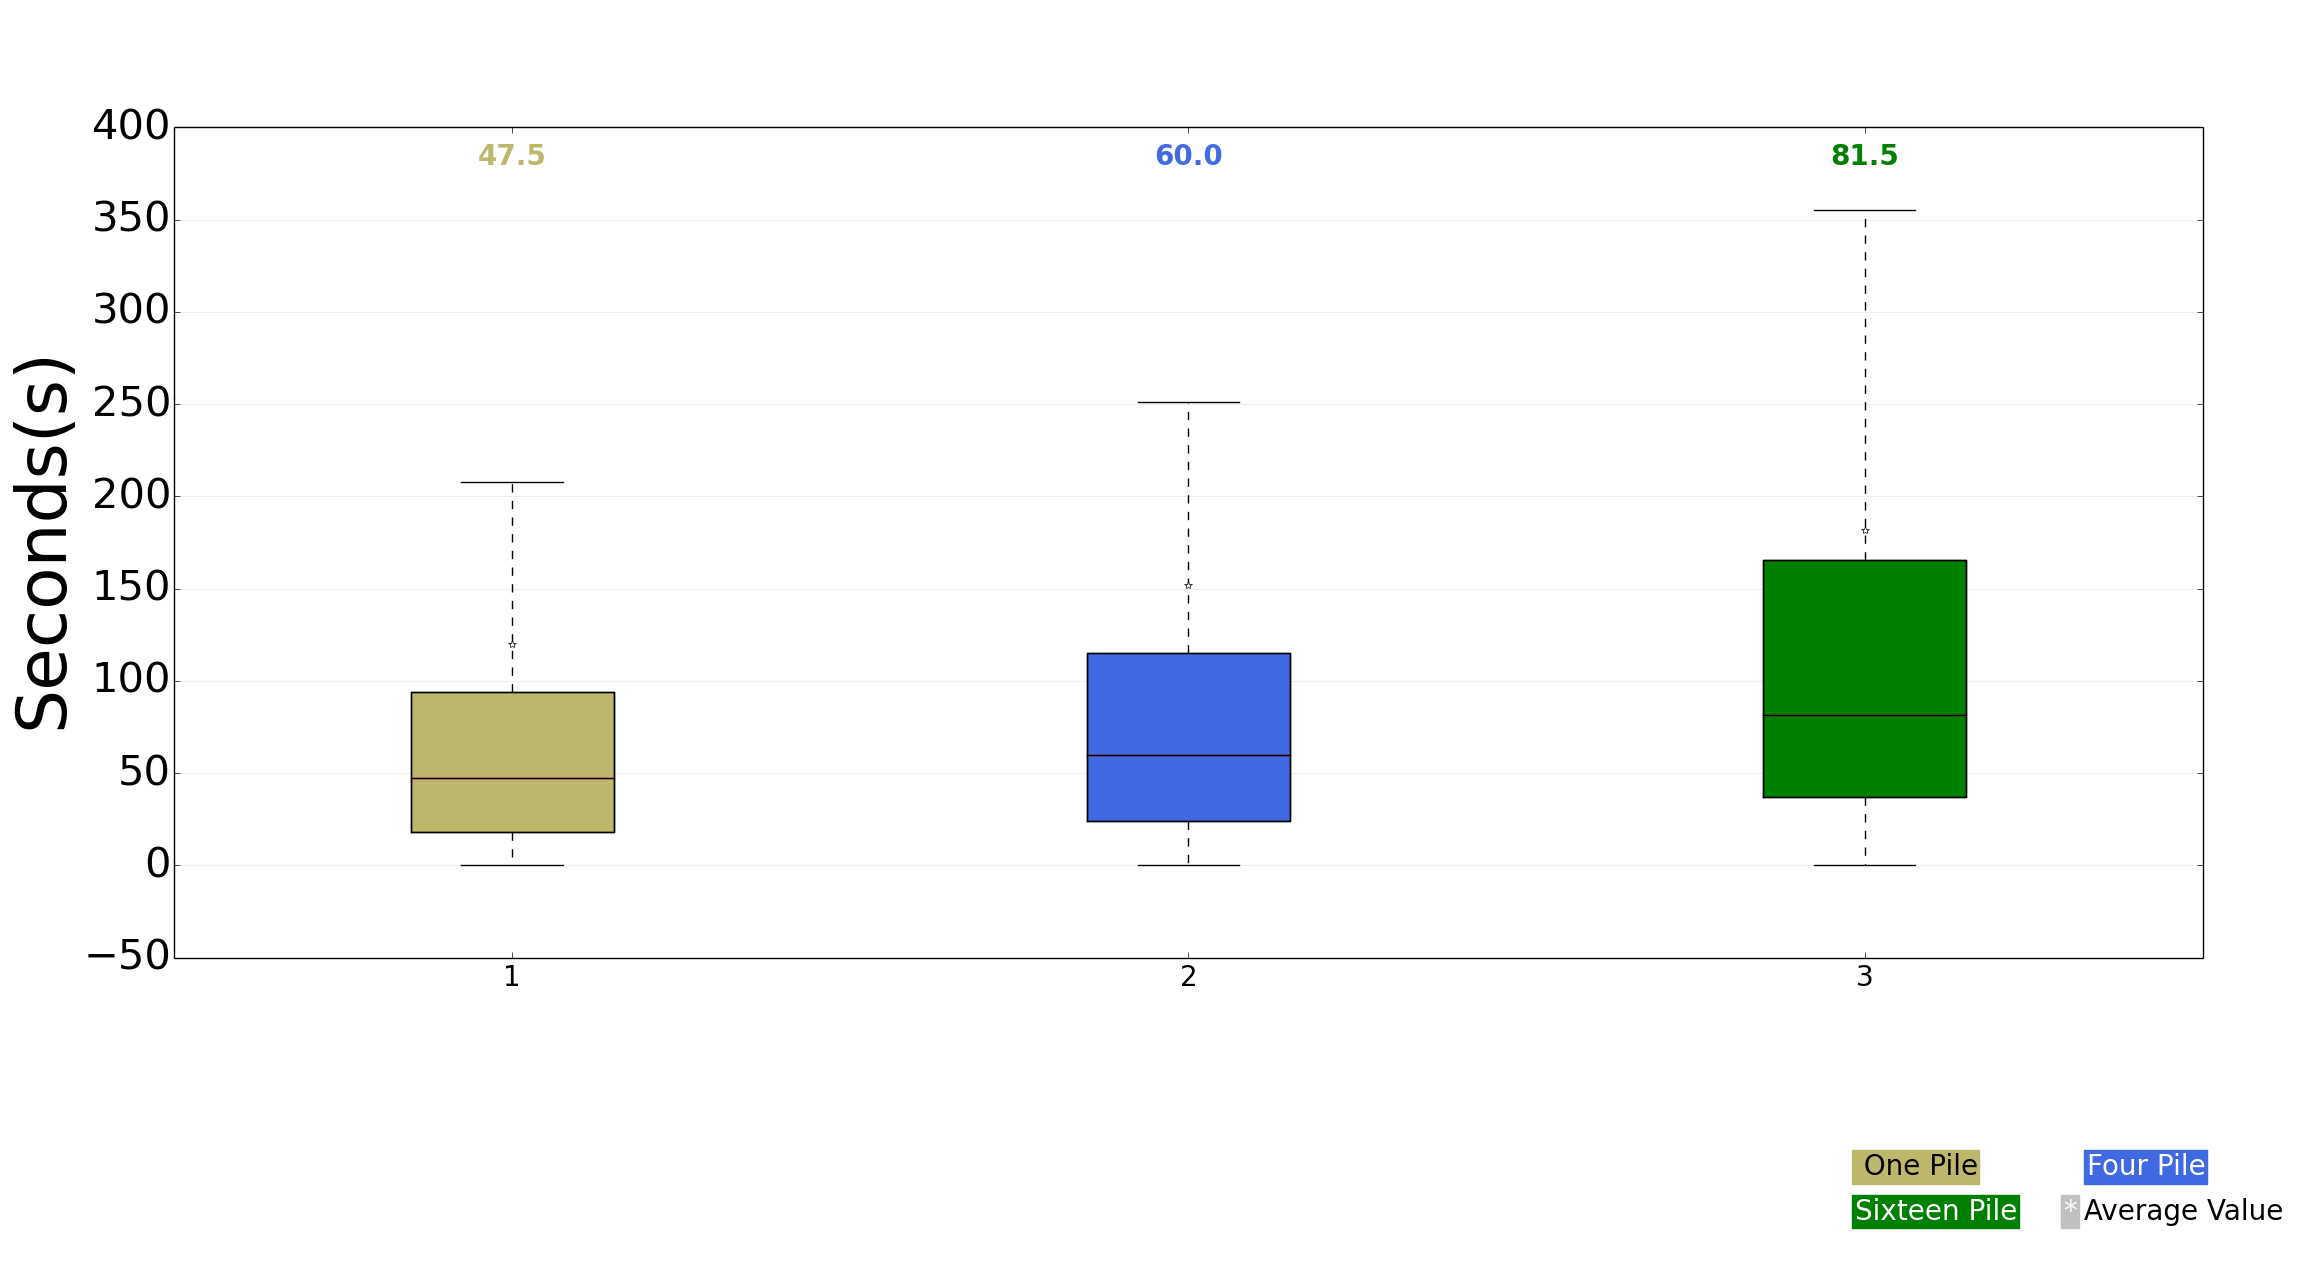
\includegraphics[width=\textwidth,height=0.35\textheight]{PheromoneOnly/ConstantWithNoOutlier.png}
	\caption{Efficiency of Constant Detrending method on data of \textit{P. rugosus} for pheromone only Settings.}
\end{figure}
\begin{figure}
	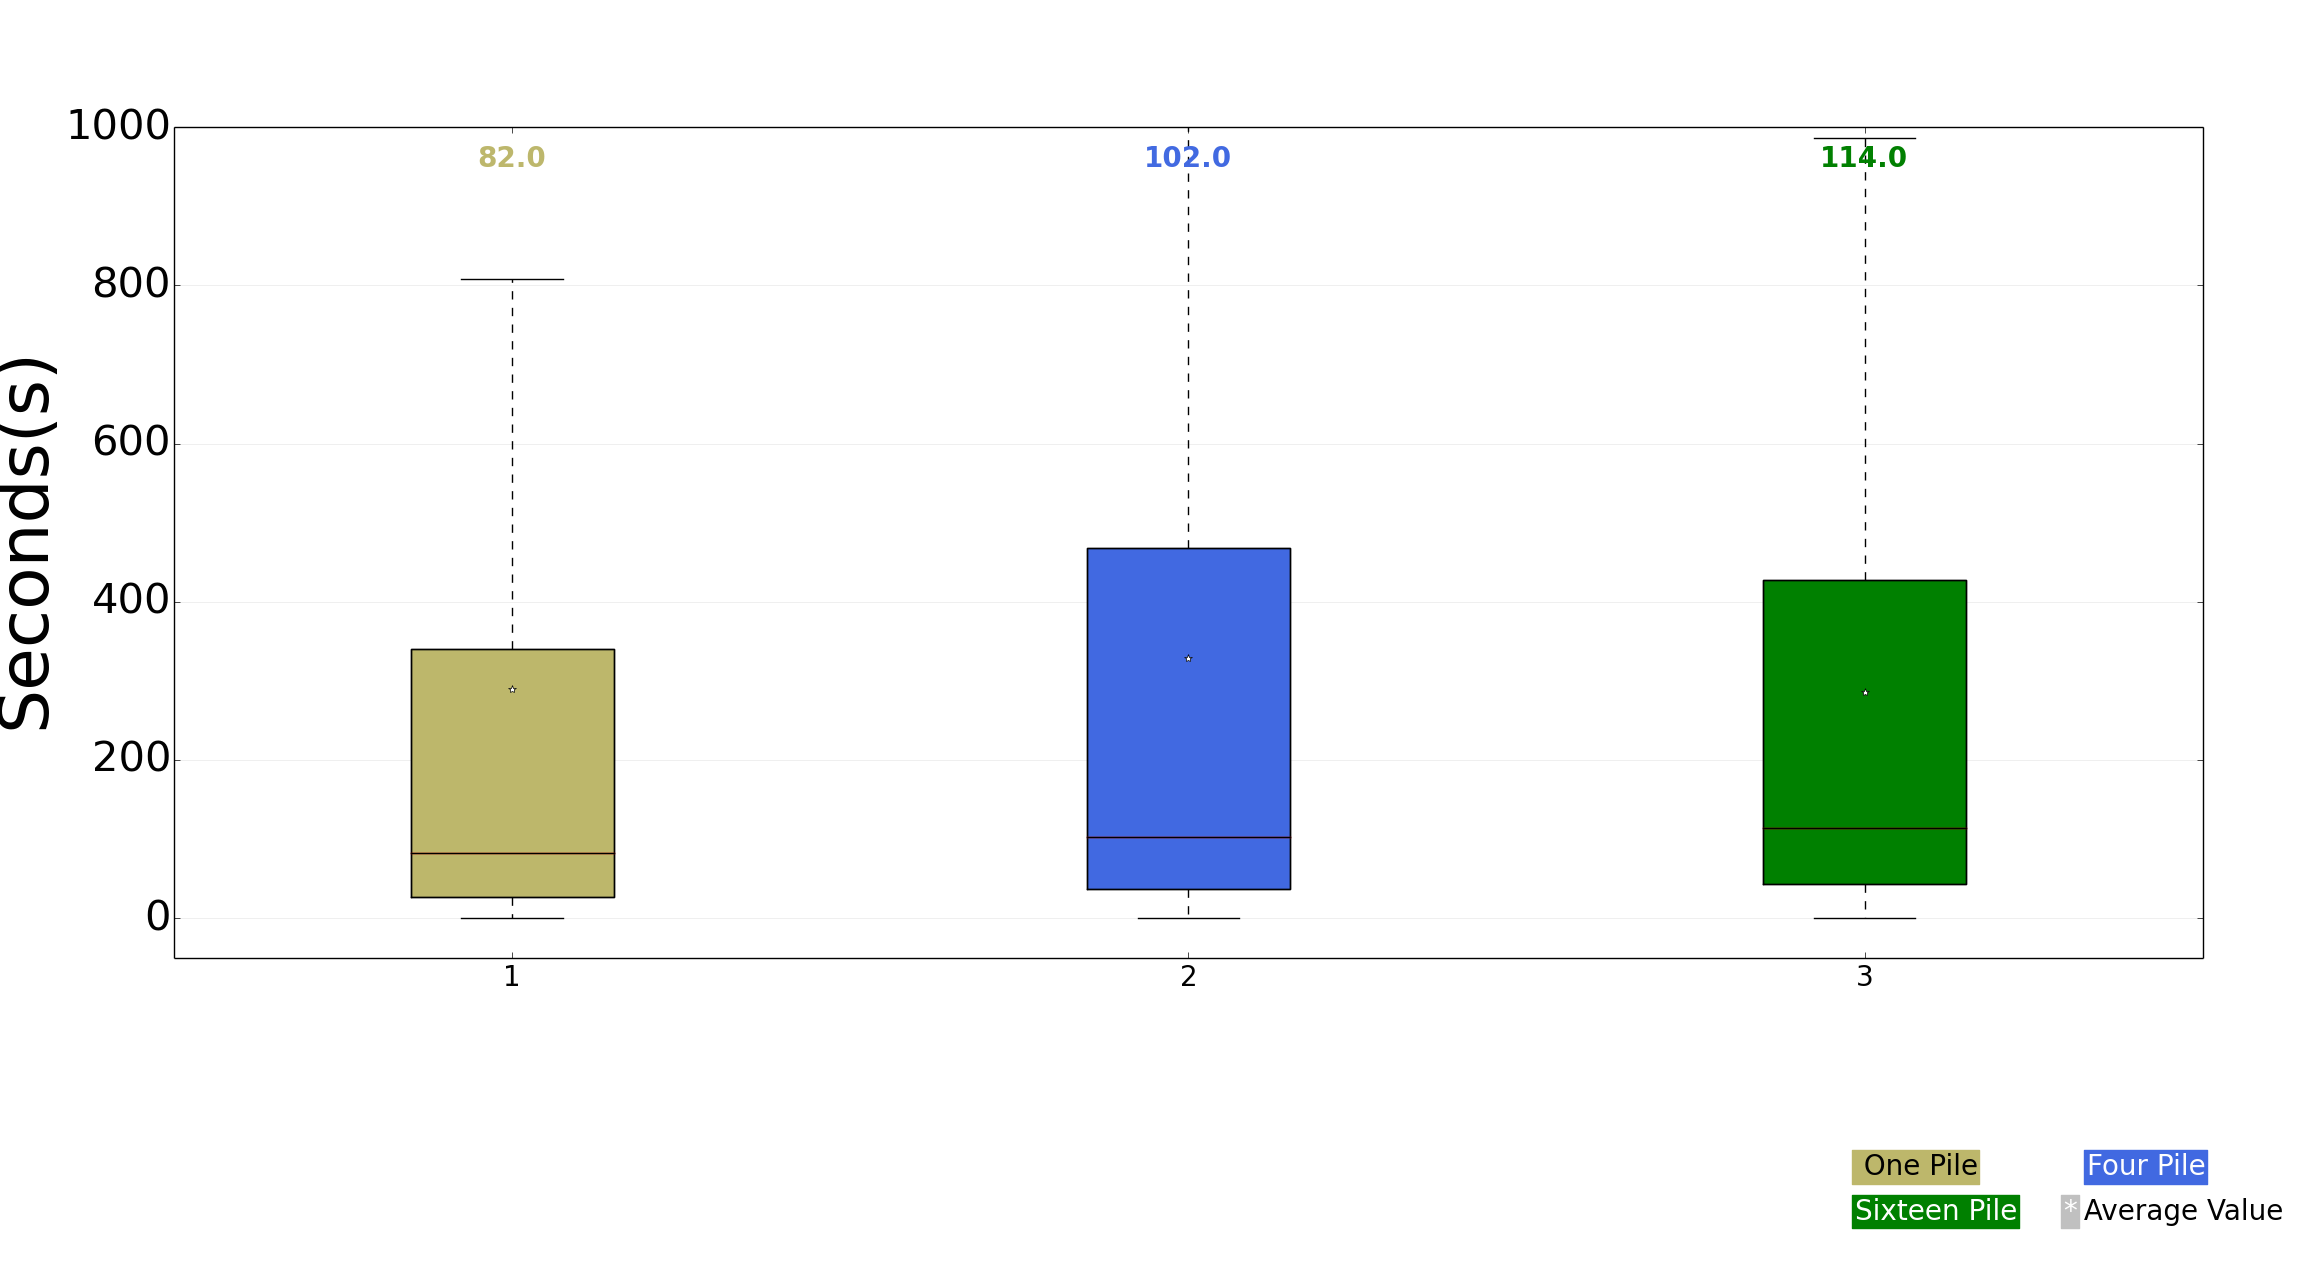
\includegraphics[width=\textwidth,height=0.35\textheight]{PheromoneOnly/LinearWithNoOutlierRateOfChange.png}
	\caption{Efficiency of Linear Detrending with rate of change method on data of \textit{P. rugosus} for pheromone only settings.}
\end{figure}
\begin{figure}
	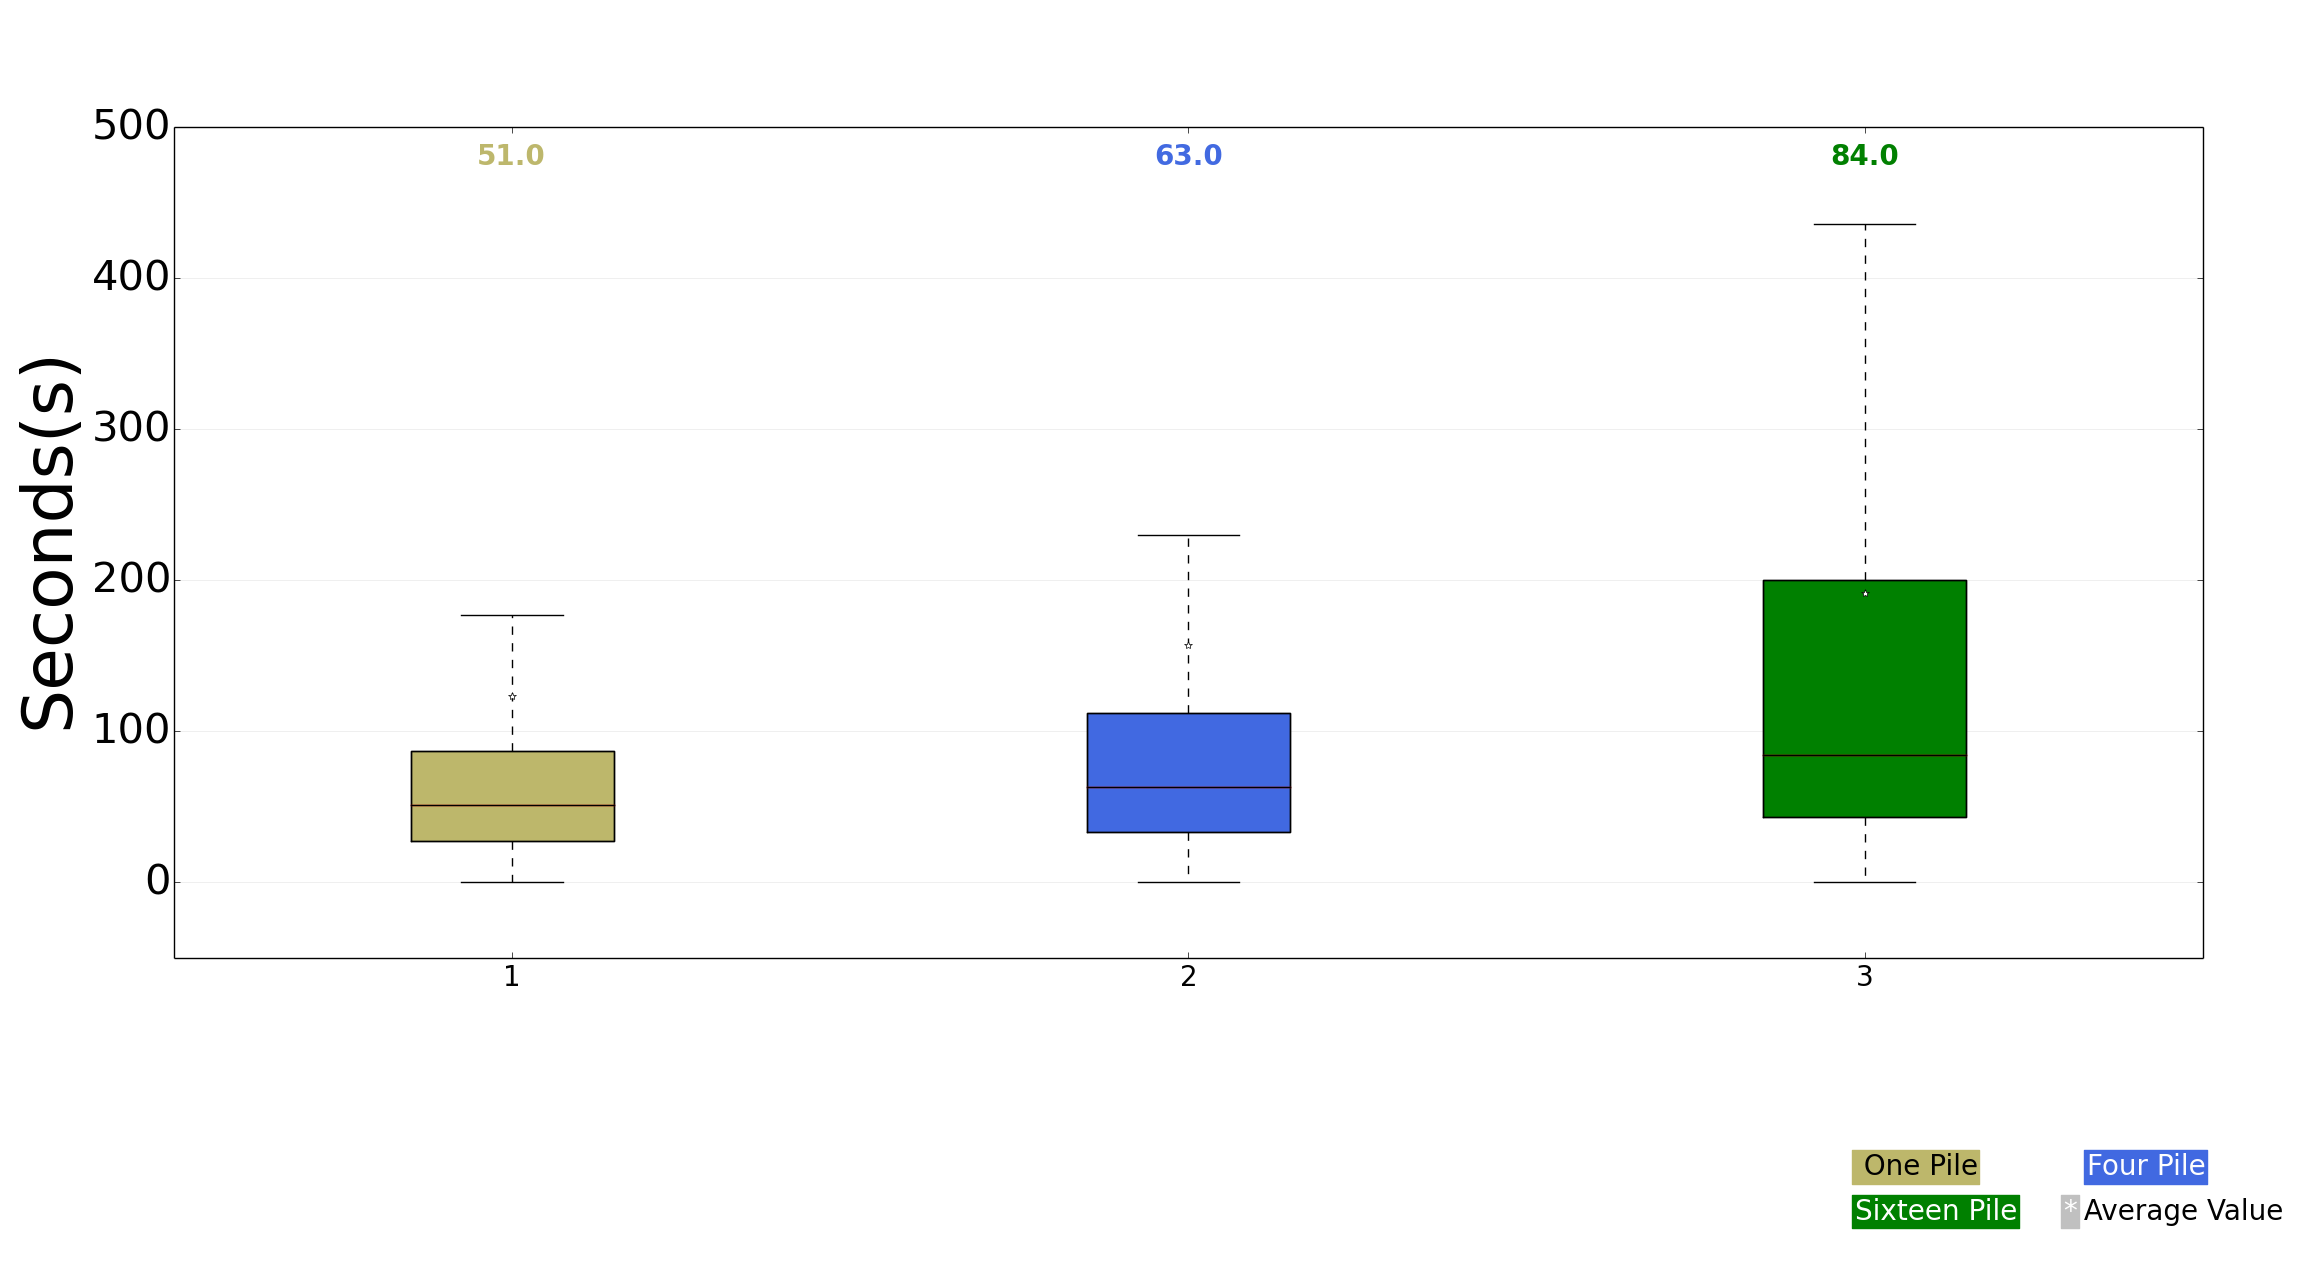
\includegraphics[width=\textwidth,height=0.35\textheight]{PheromoneOnly/ConsantWithNoOutlierRateOfChange.png}
	\caption{Efficiency of Linear Detrending with rate of change method on data of \textit{P. rugosus} for pheromone only settings}
\end{figure}
\begin{figure}
	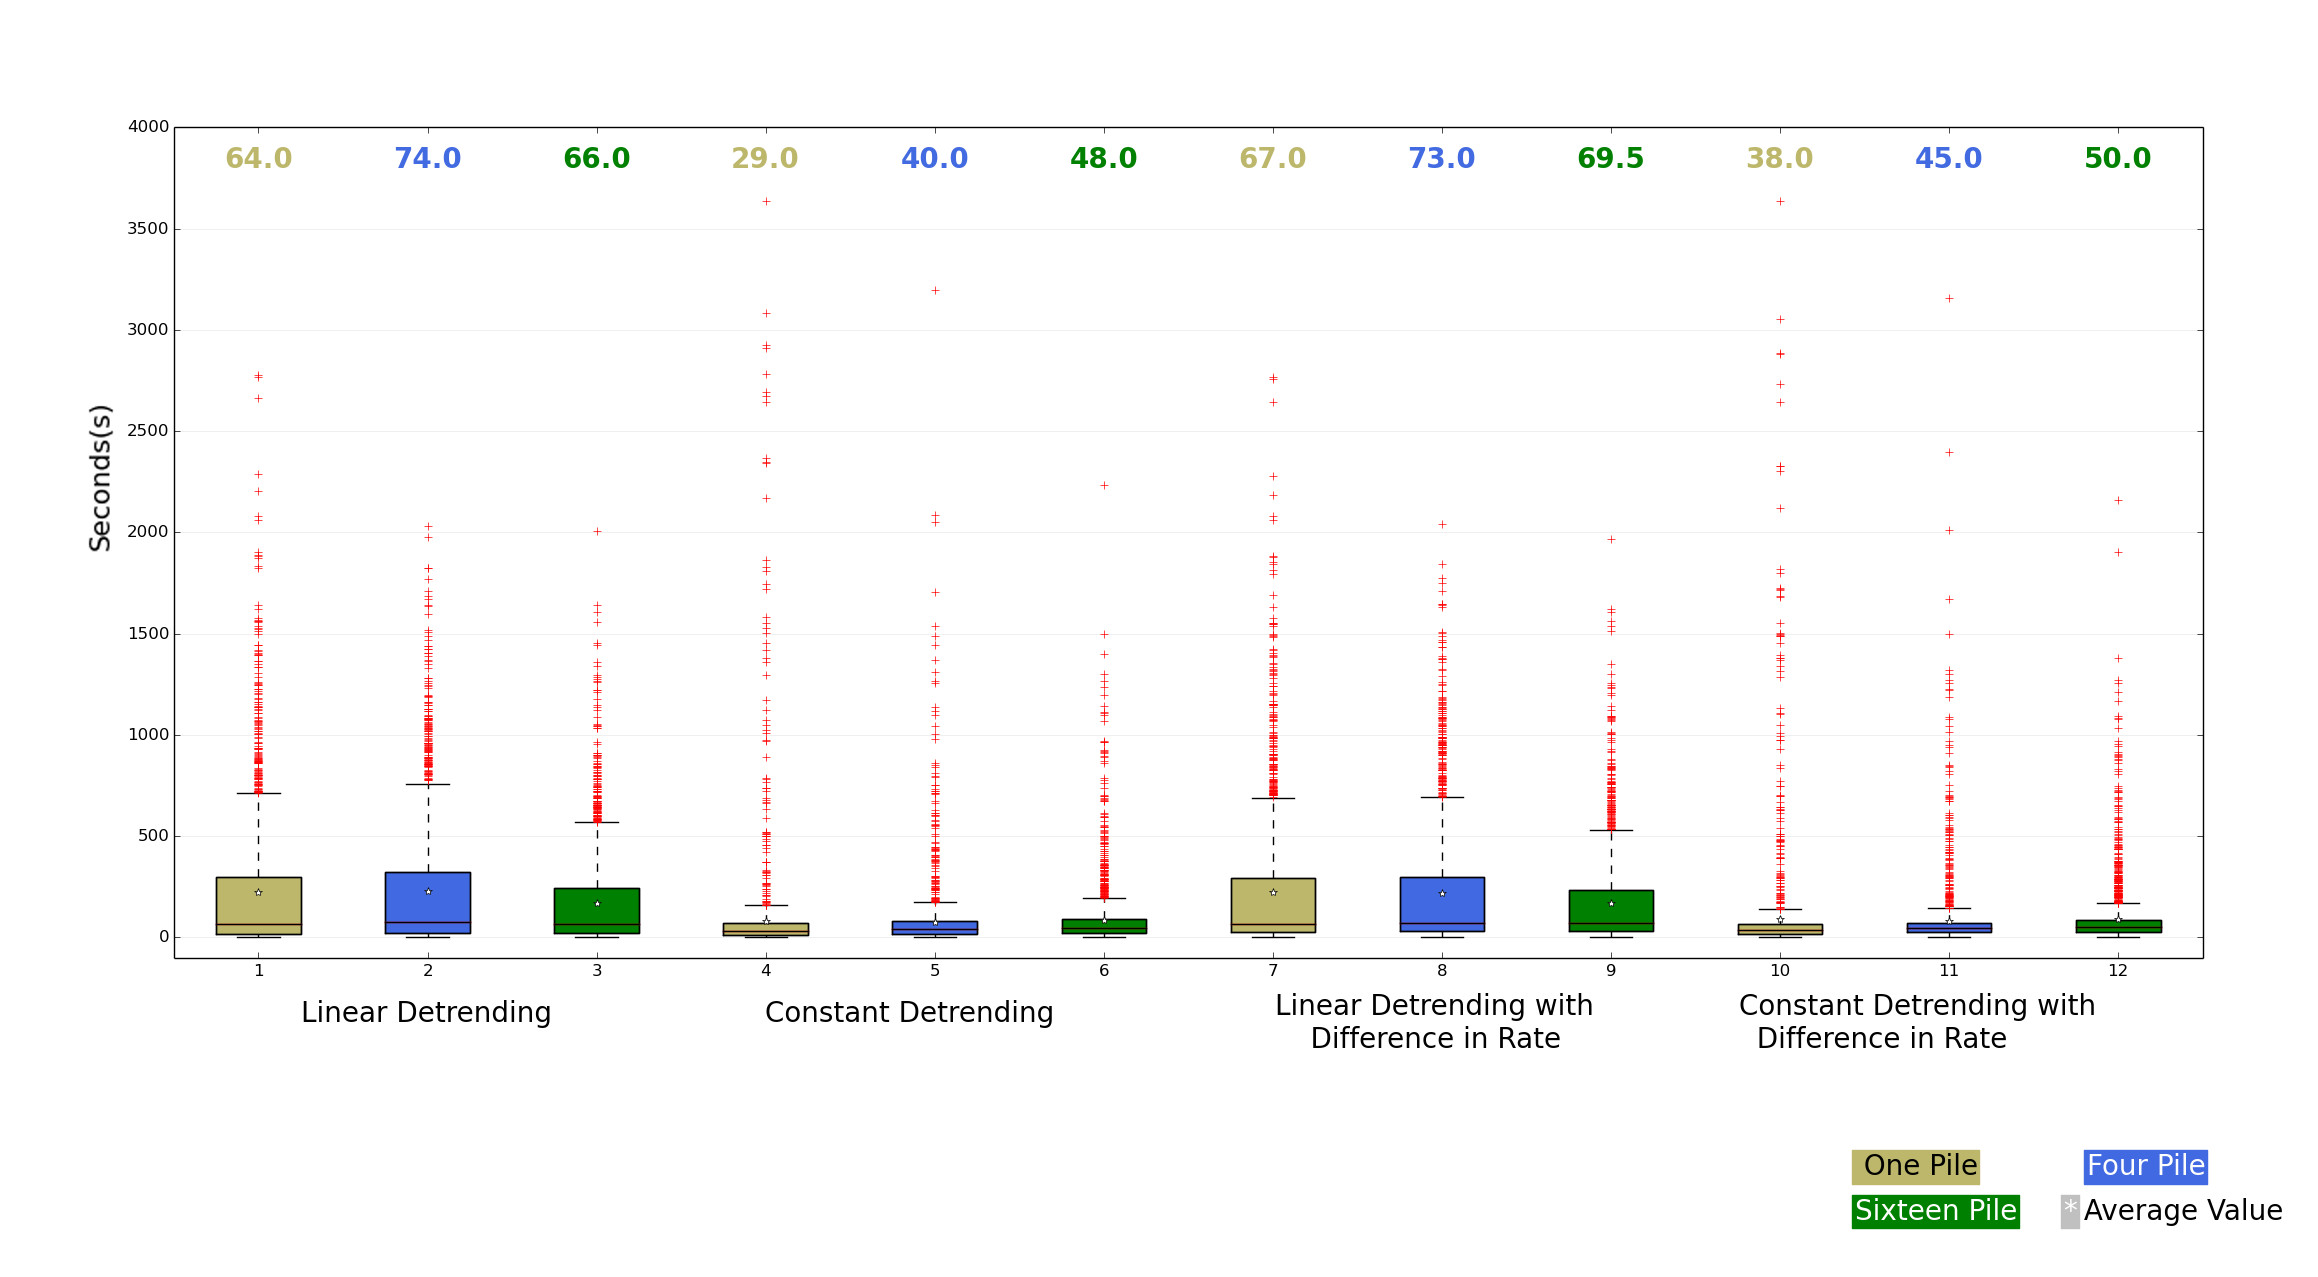
\includegraphics[width=\textwidth,height=0.35\textheight]{AllParameters/AllPlotComparison.png}
	\caption{Comparison of all methods on data of \textit{P. rugosus} for both combination of communication and memory}
\end{figure}
\begin{figure}
	\includegraphics[width=\textwidth,height=0.35\textheight]{AllParameters/AllPlot.png}
	\caption{Comparison of all methods without outliers on data of \textit{P. rugosus} for both combination of communication and memory}
\end{figure}
\begin{figure}
	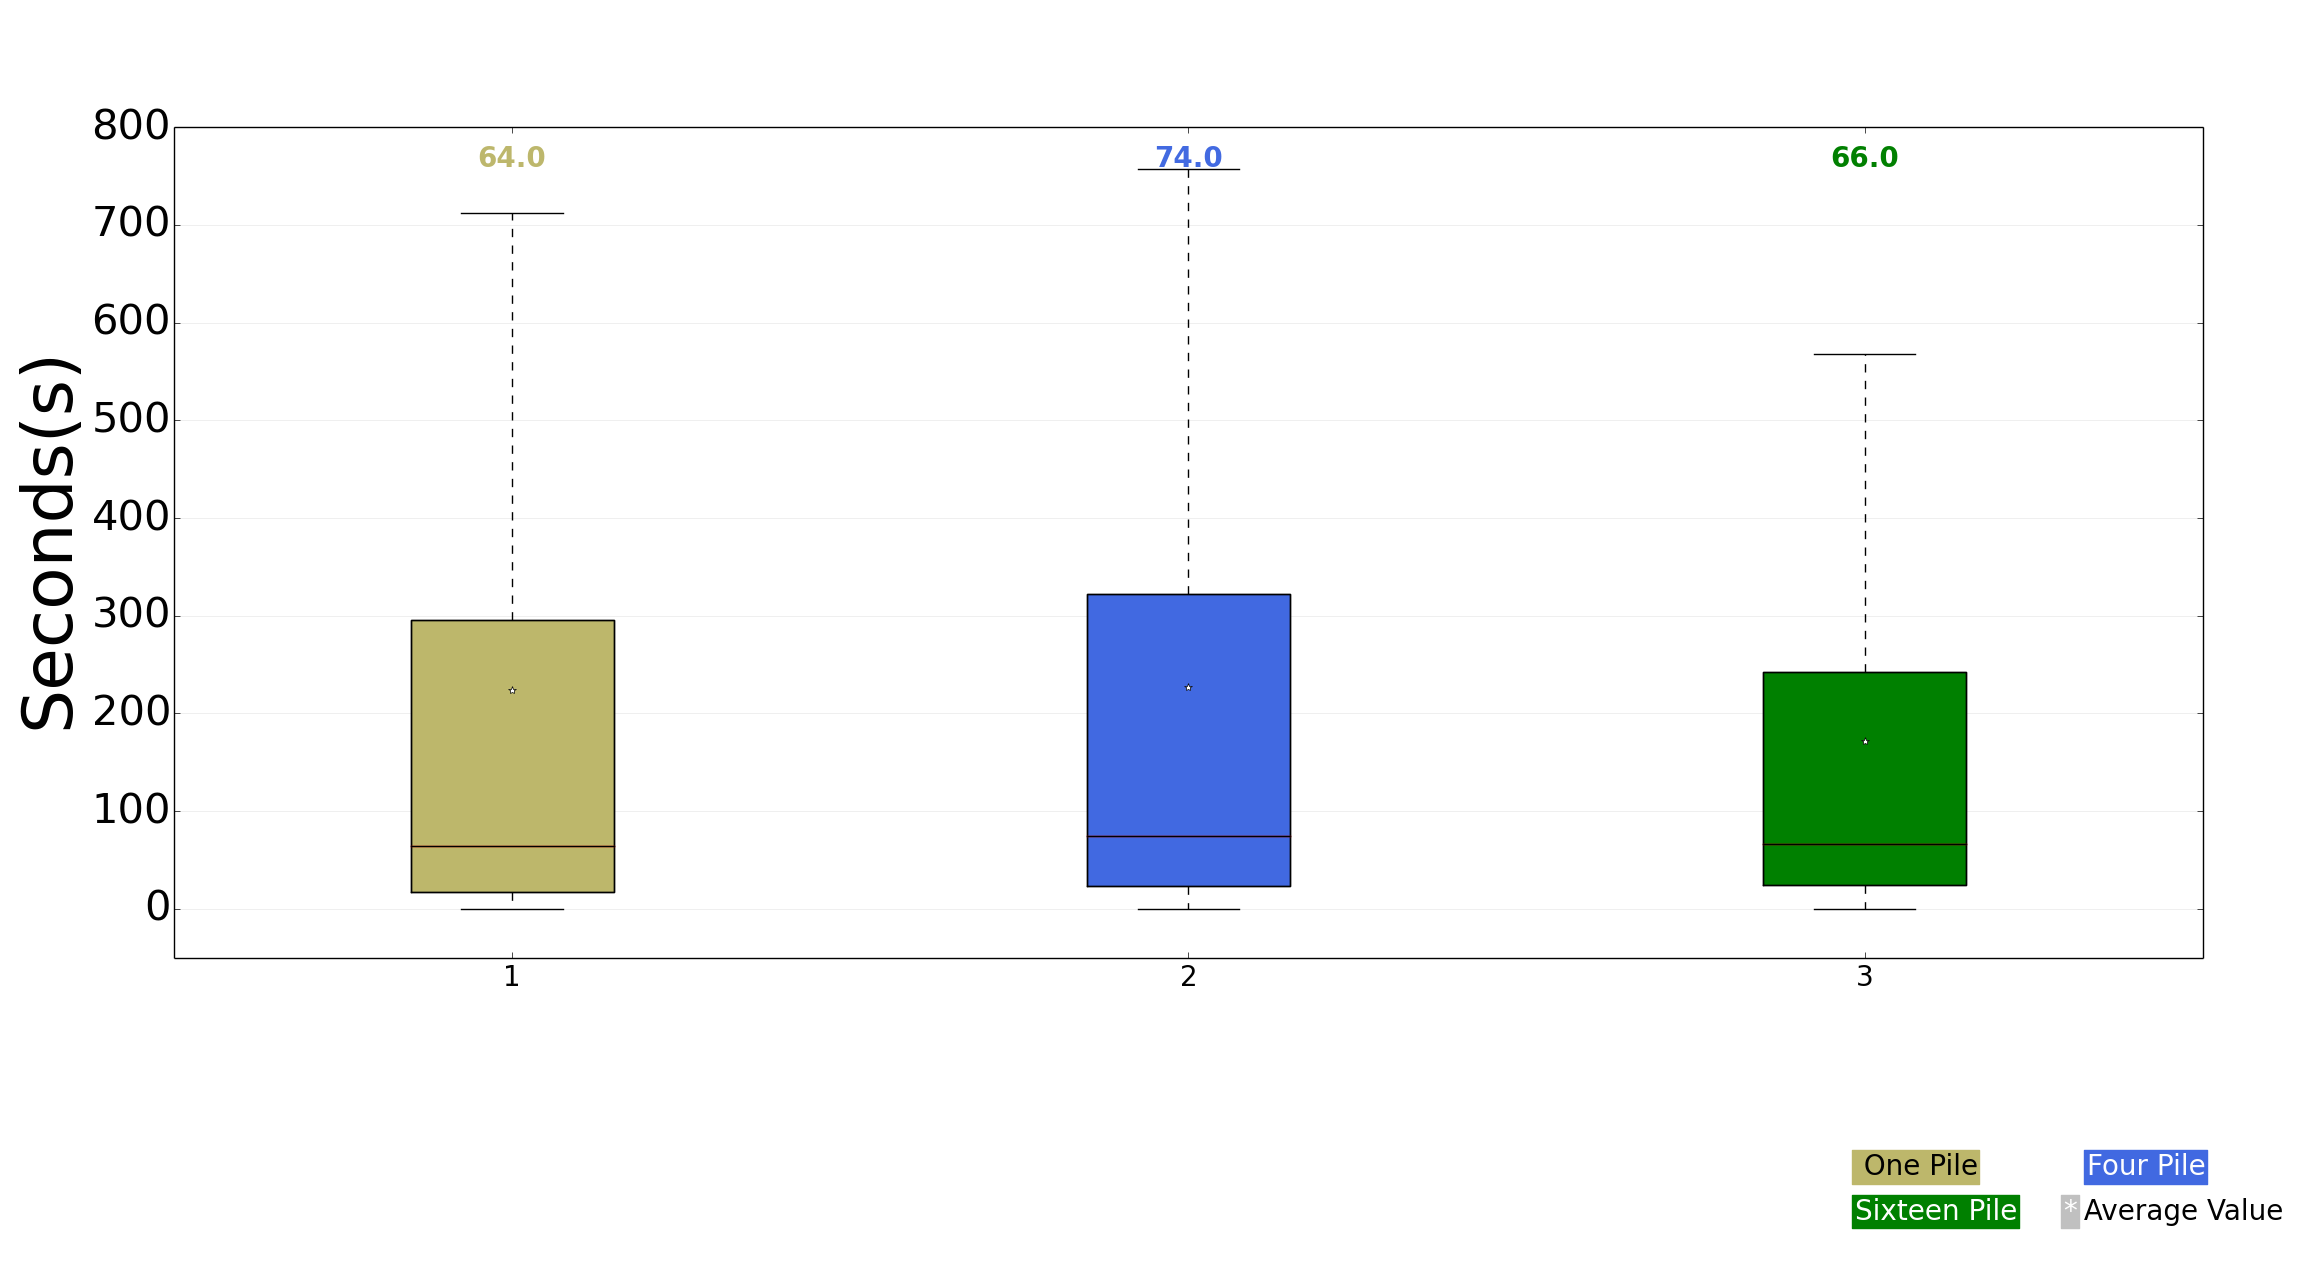
\includegraphics[width=\textwidth,height=0.35\textheight]{AllParameters/LinearDetrendingNoOutlier.png}
	\caption{Efficiency of linear detrending on data of \textit{P. rugosus} for combination of communication and sitefidelity }
\end{figure}
\begin{figure}
	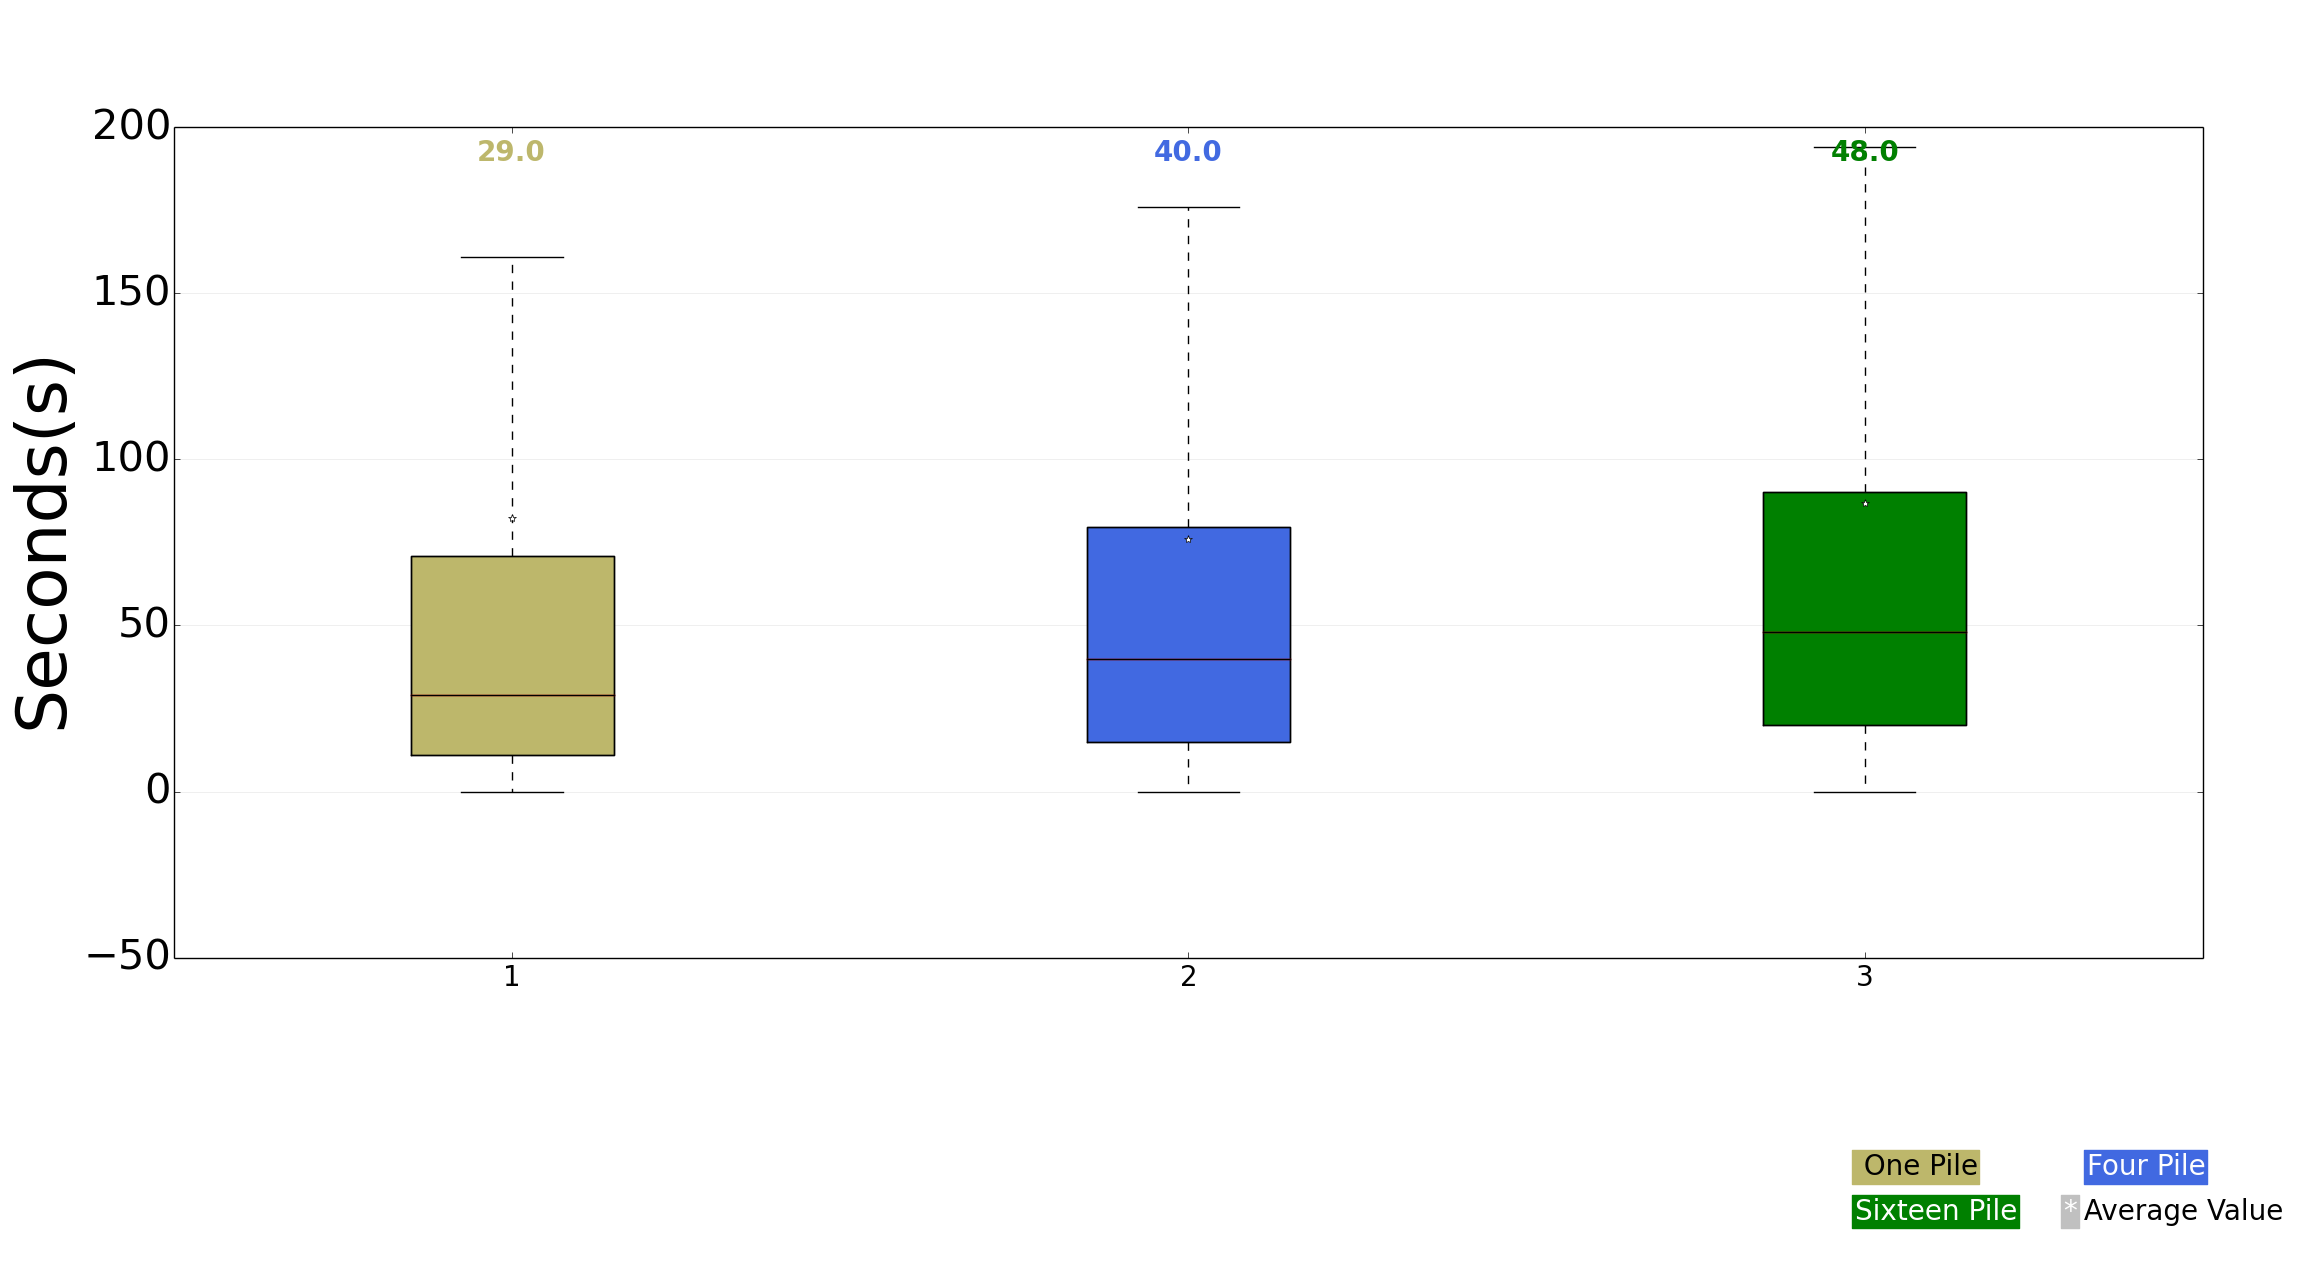
\includegraphics[width=\textwidth,height=0.35\textheight]{AllParameters/ConstantDetrendingNoOutlier.png}
	\caption{Efficiency of constant detrending methods on data of \textit{P. rugosus} for both combination of communication and memory}
\end{figure}
\begin{figure}
	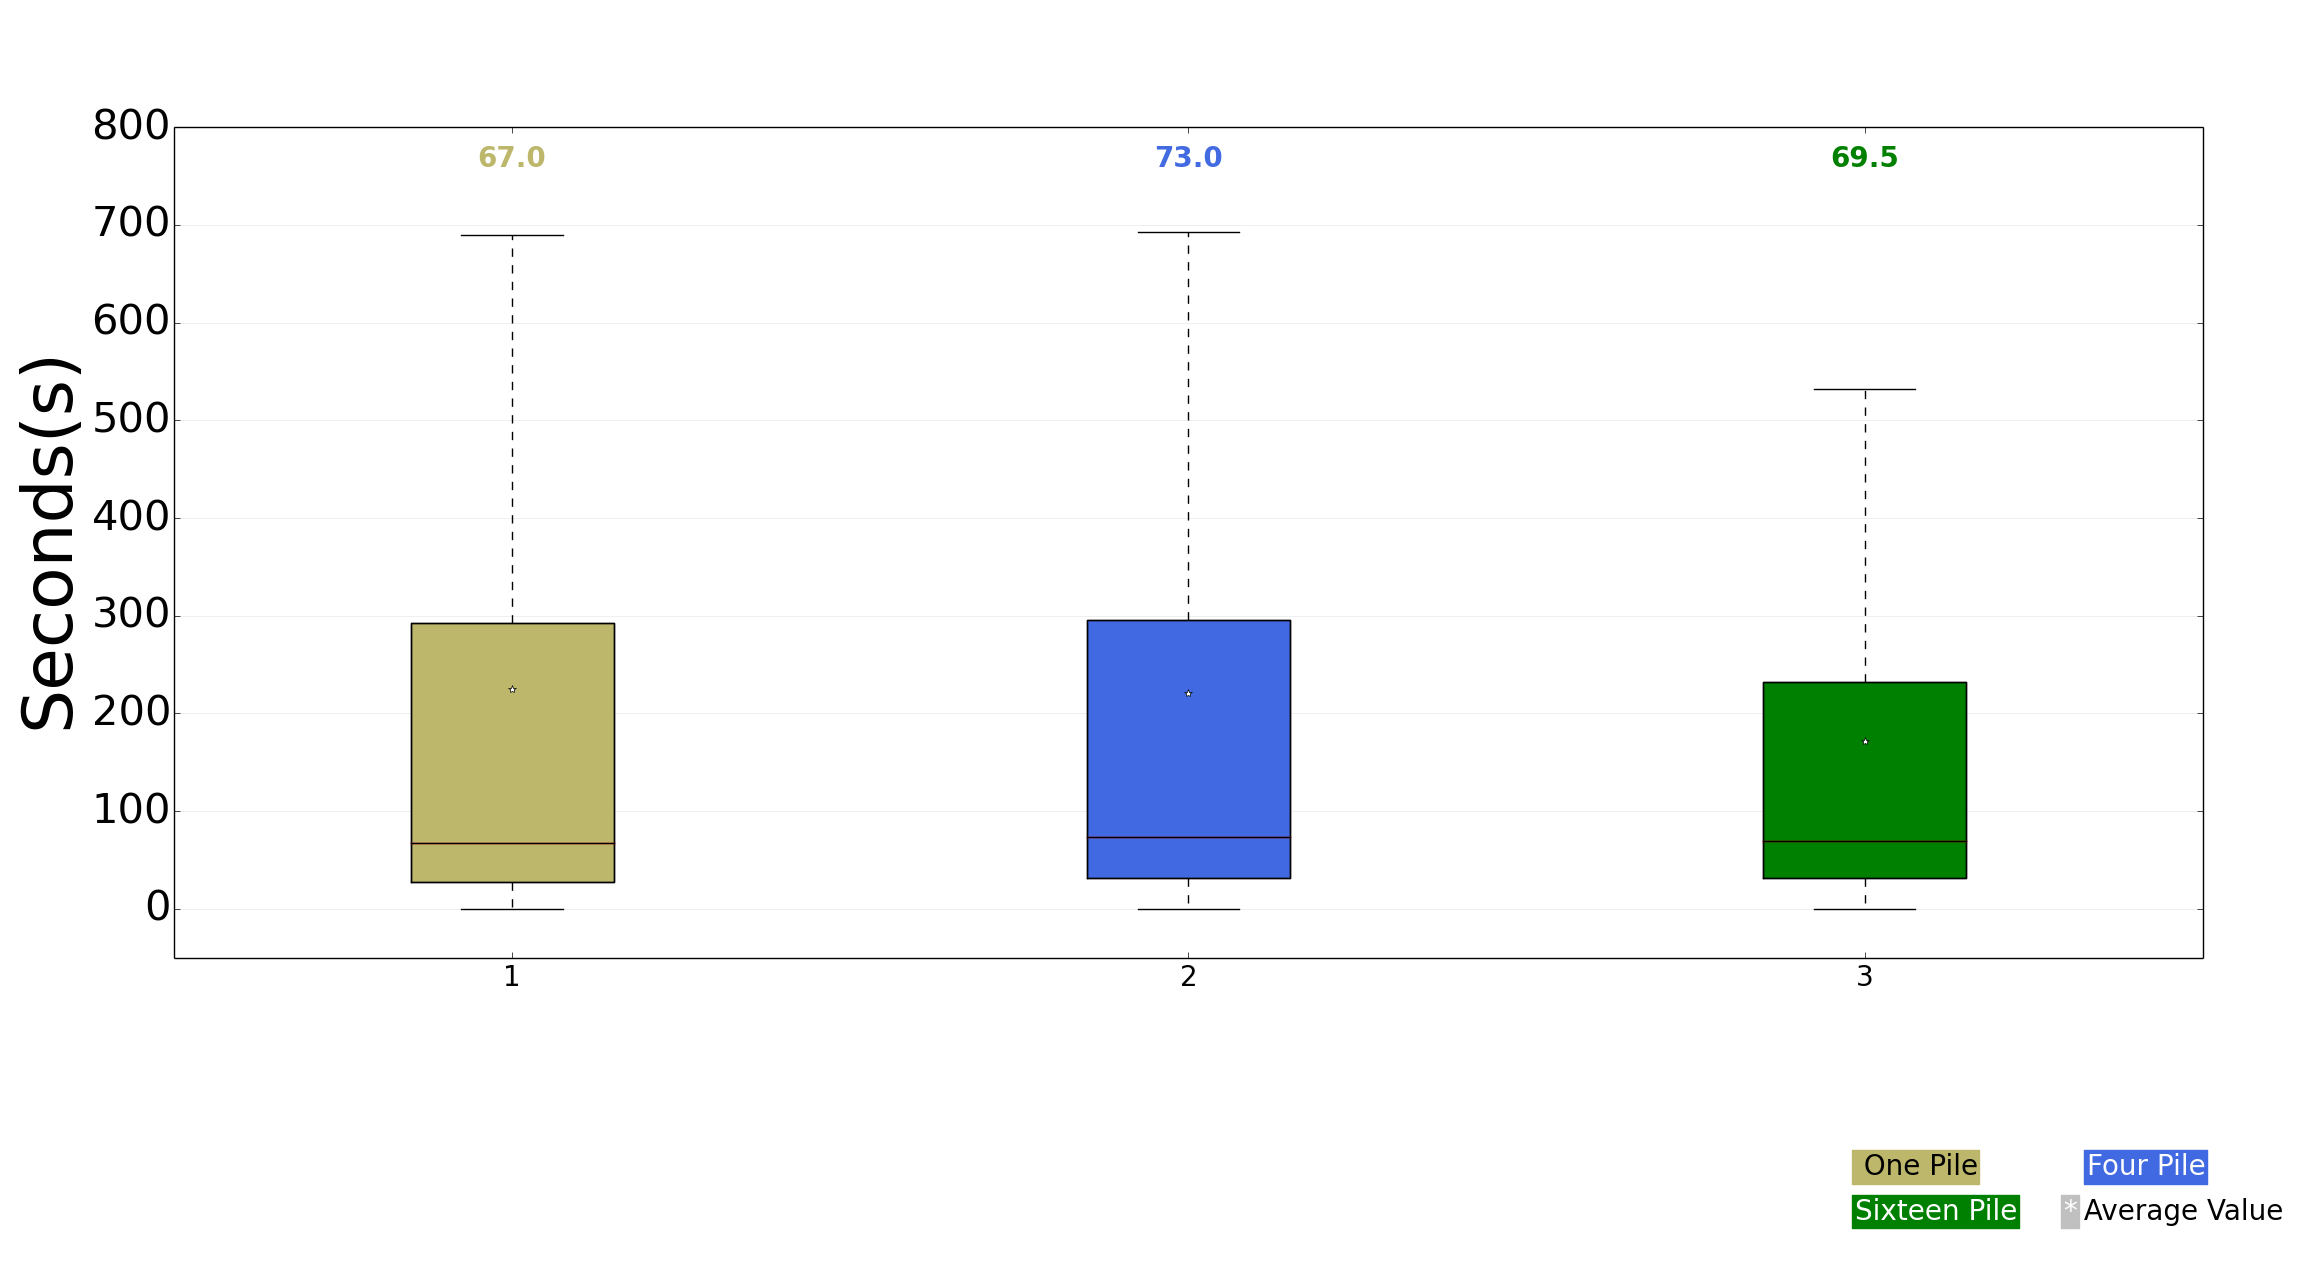
\includegraphics[width=\textwidth,height=0.35\textheight]{AllParameters/LinearDetrendingNoOutlierRateOfChange.png}
	\caption{Efficiency of linear detrending method with rate of change in foraging rate on data of \textit{P. rugosus} for both combination of communication and memory}
\end{figure}
\begin{figure}
	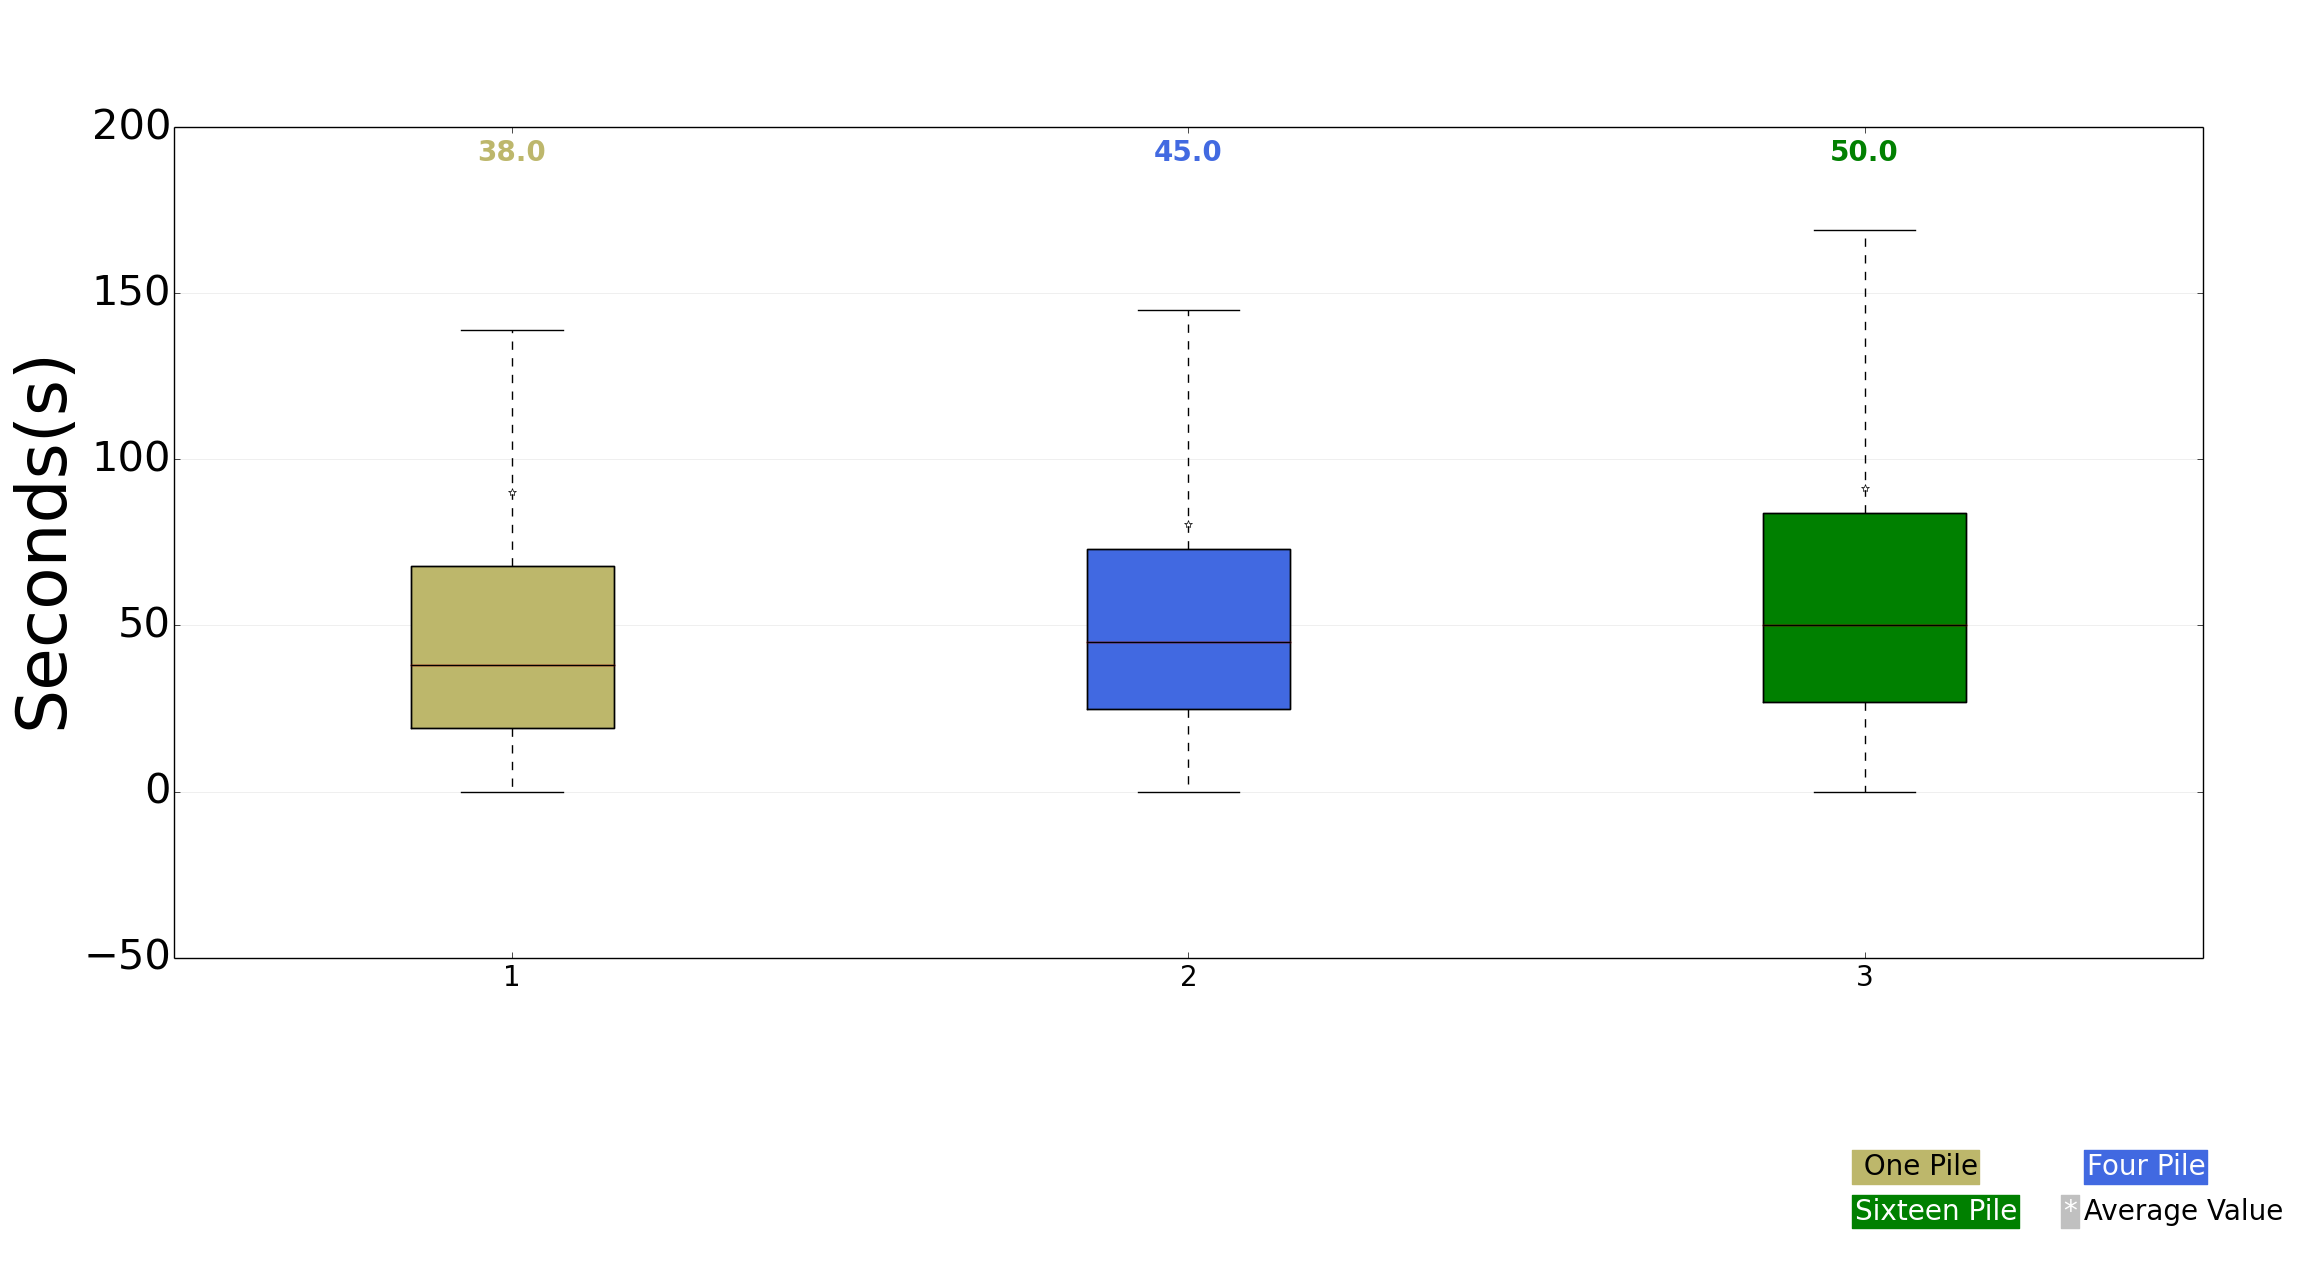
\includegraphics[width=\textwidth,height=0.35\textheight]{AllParameters/ConstantDetrendingNoOutlierRateOfChange.png}
	\caption{Efficiency of constant detrending method with rate of change in foraging rate on data of \textit{P. rugosus} for both combination of communication and memory}
\end{figure}
\begin{figure}
	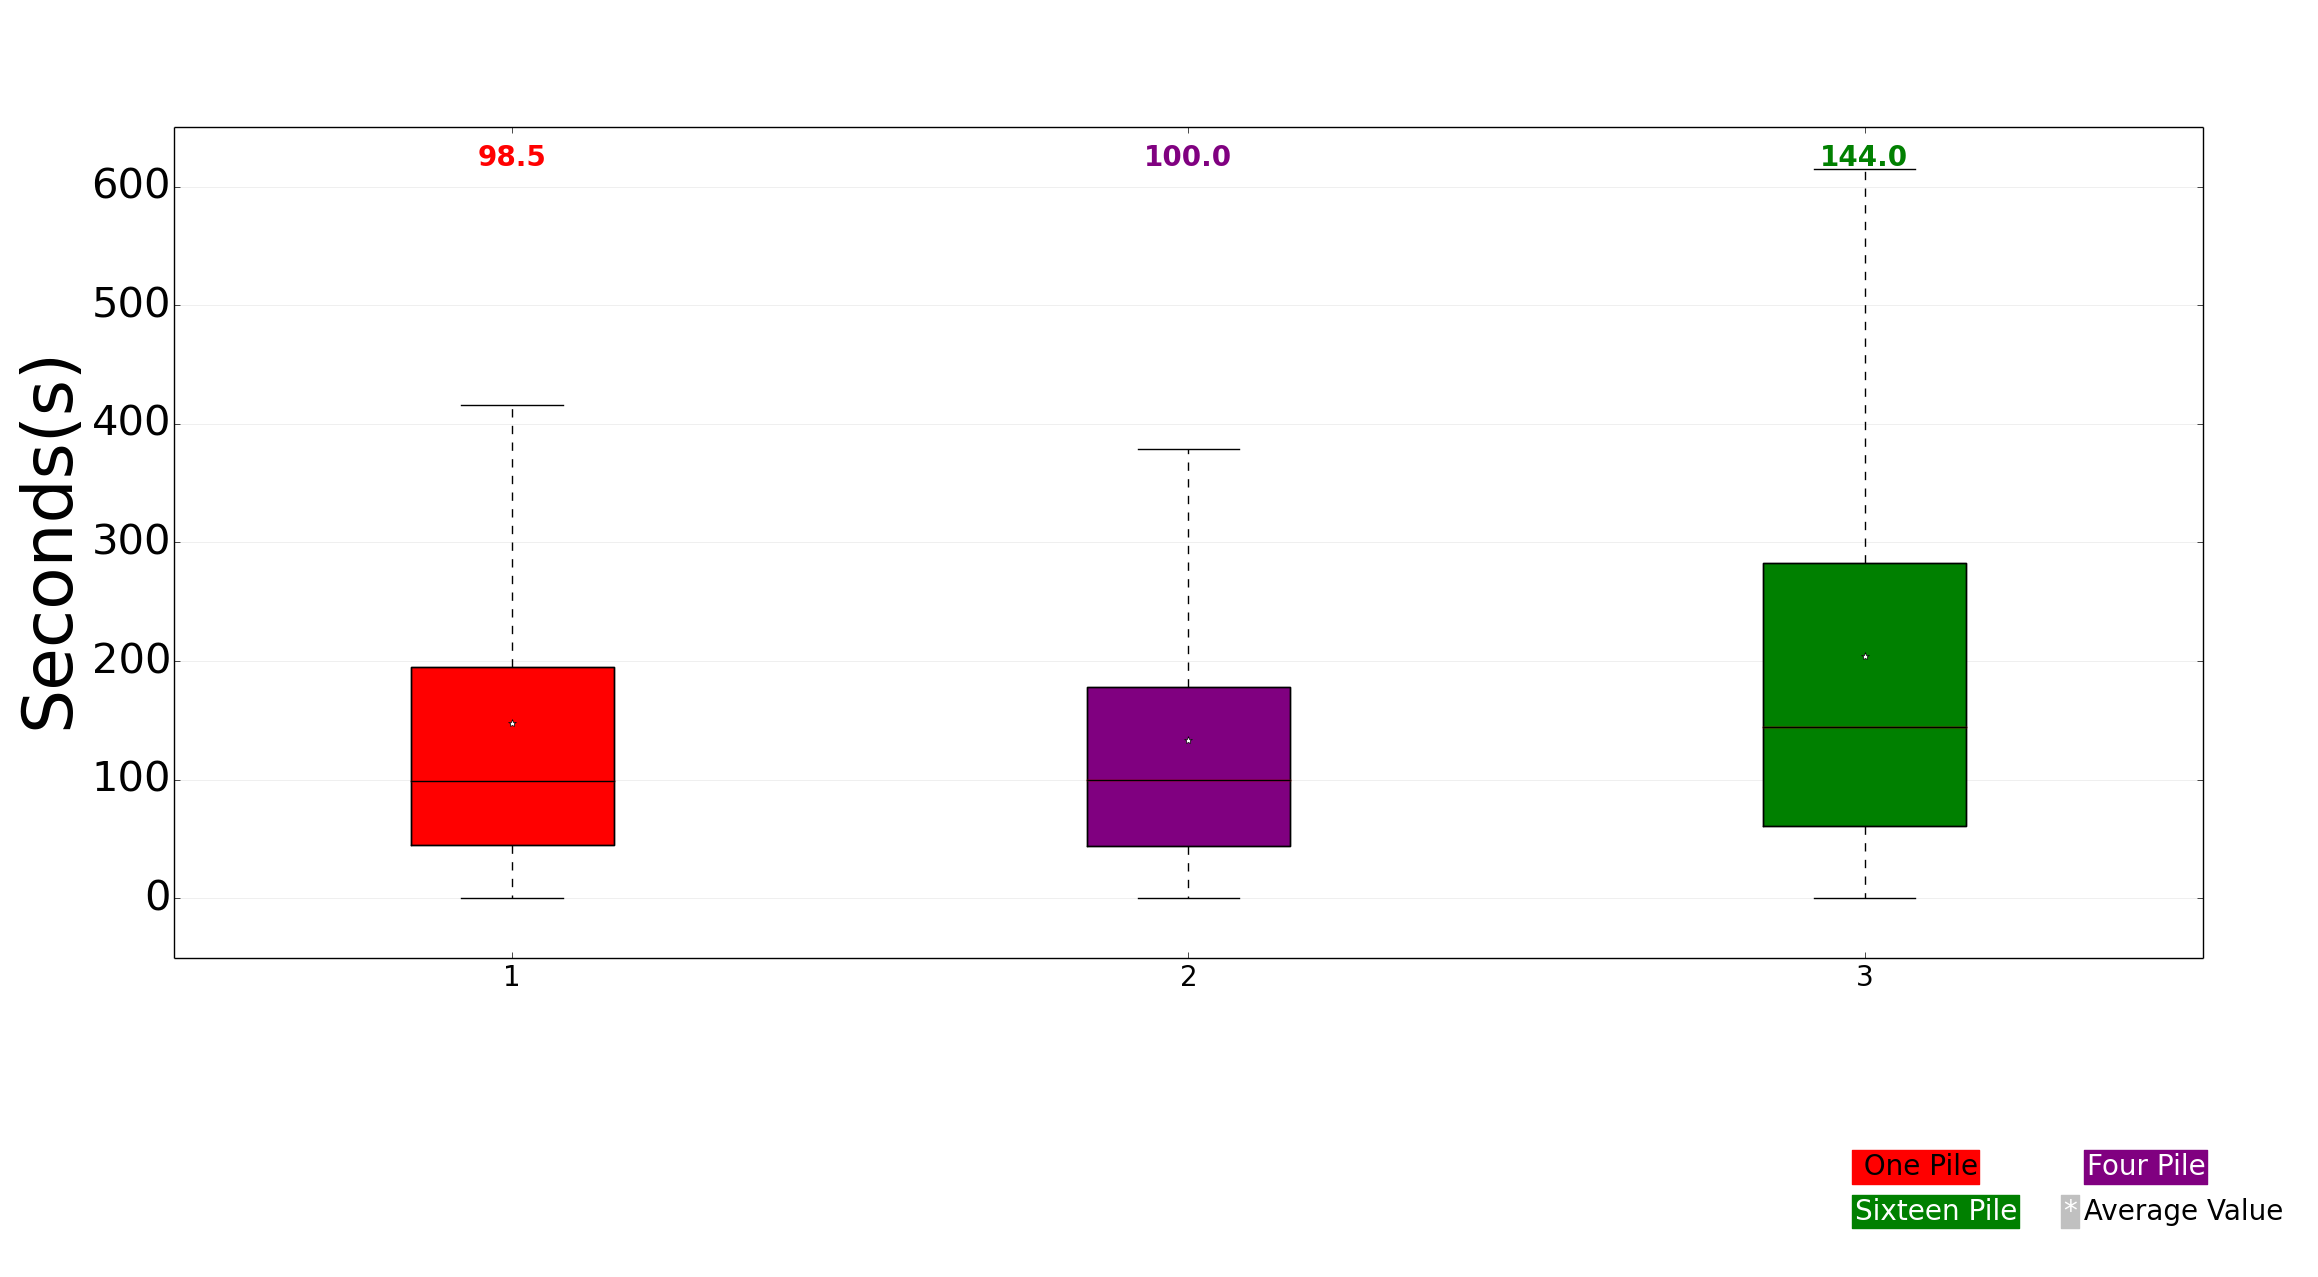
\includegraphics[width=\textwidth,height=0.35\textheight]{AllParameters/RawFit/BoxPlot_NoDetrend_96Ants_ChangeFRate.png}
	\caption{Efficiency of change point detection algorithm on foraging rate for 96 ants for combination of communication and memory}
\end{figure}
\begin{figure}
	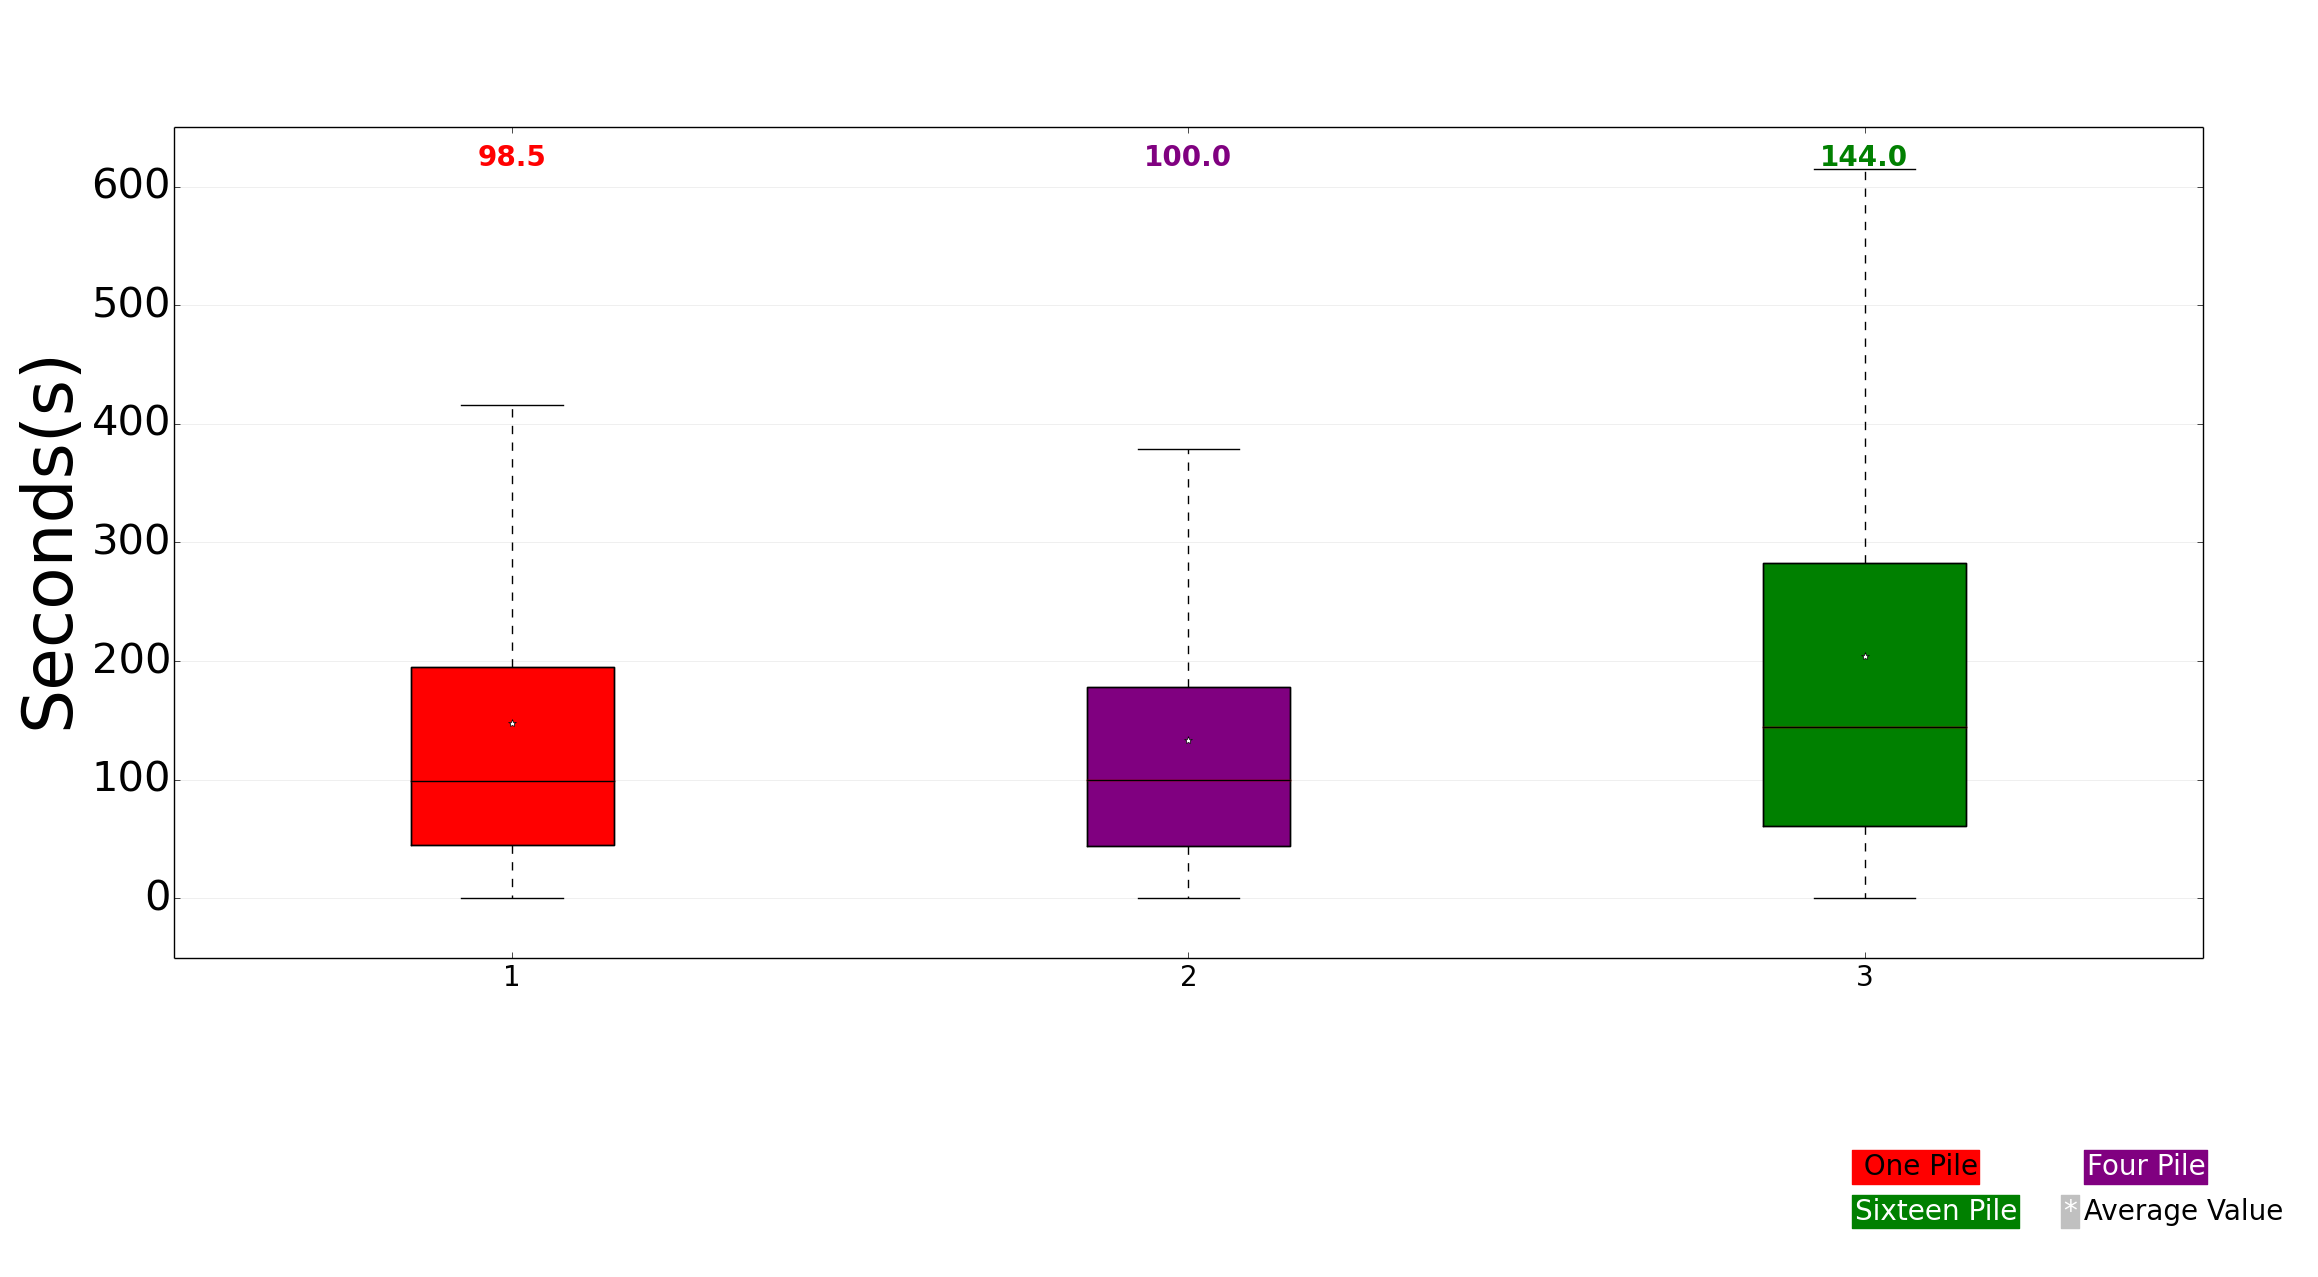
\includegraphics[width=\textwidth,height=0.35\textheight]{AllParameters/RawFit/BoxPlot_NoDetrend_96Ants_ChangeFRate.png}
	\caption{Efficiency of change point detection algorithm on change in foraging rate for 96 ants for combination of communication and memory}
\end{figure}
\begin{figure}
	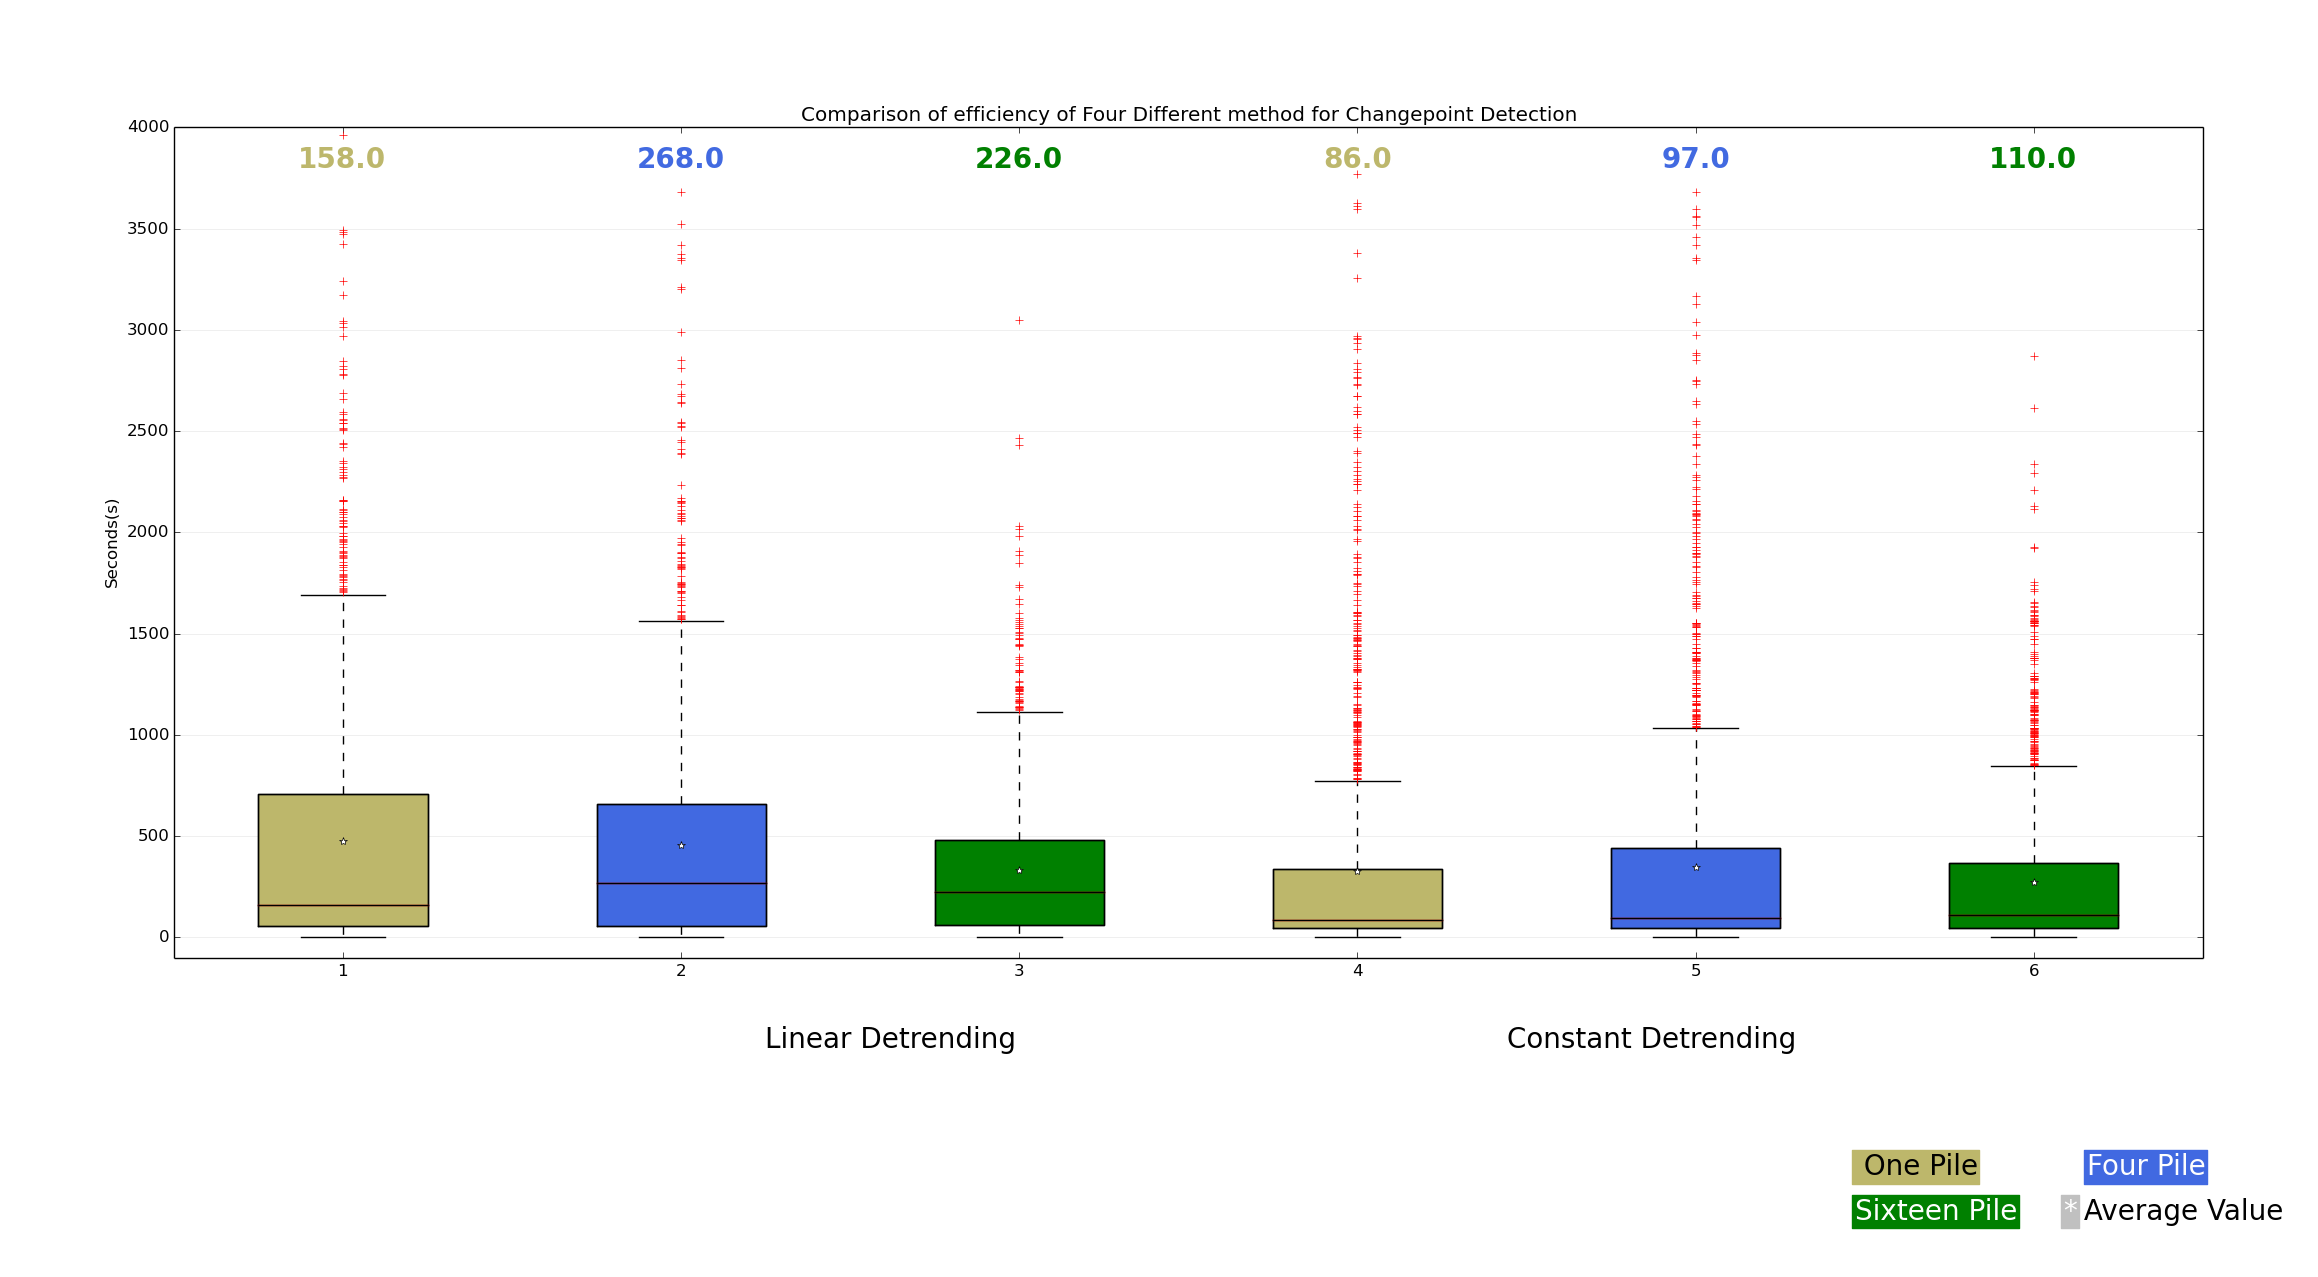
\includegraphics[width=\textwidth,height=0.35\textheight]{SiteFidelityOnly/SiteFidelity_2.png}
	\caption{Comparison of all methods on data of \textit{P. rugosus} for memory only parameters}
\end{figure}
\begin{figure}
	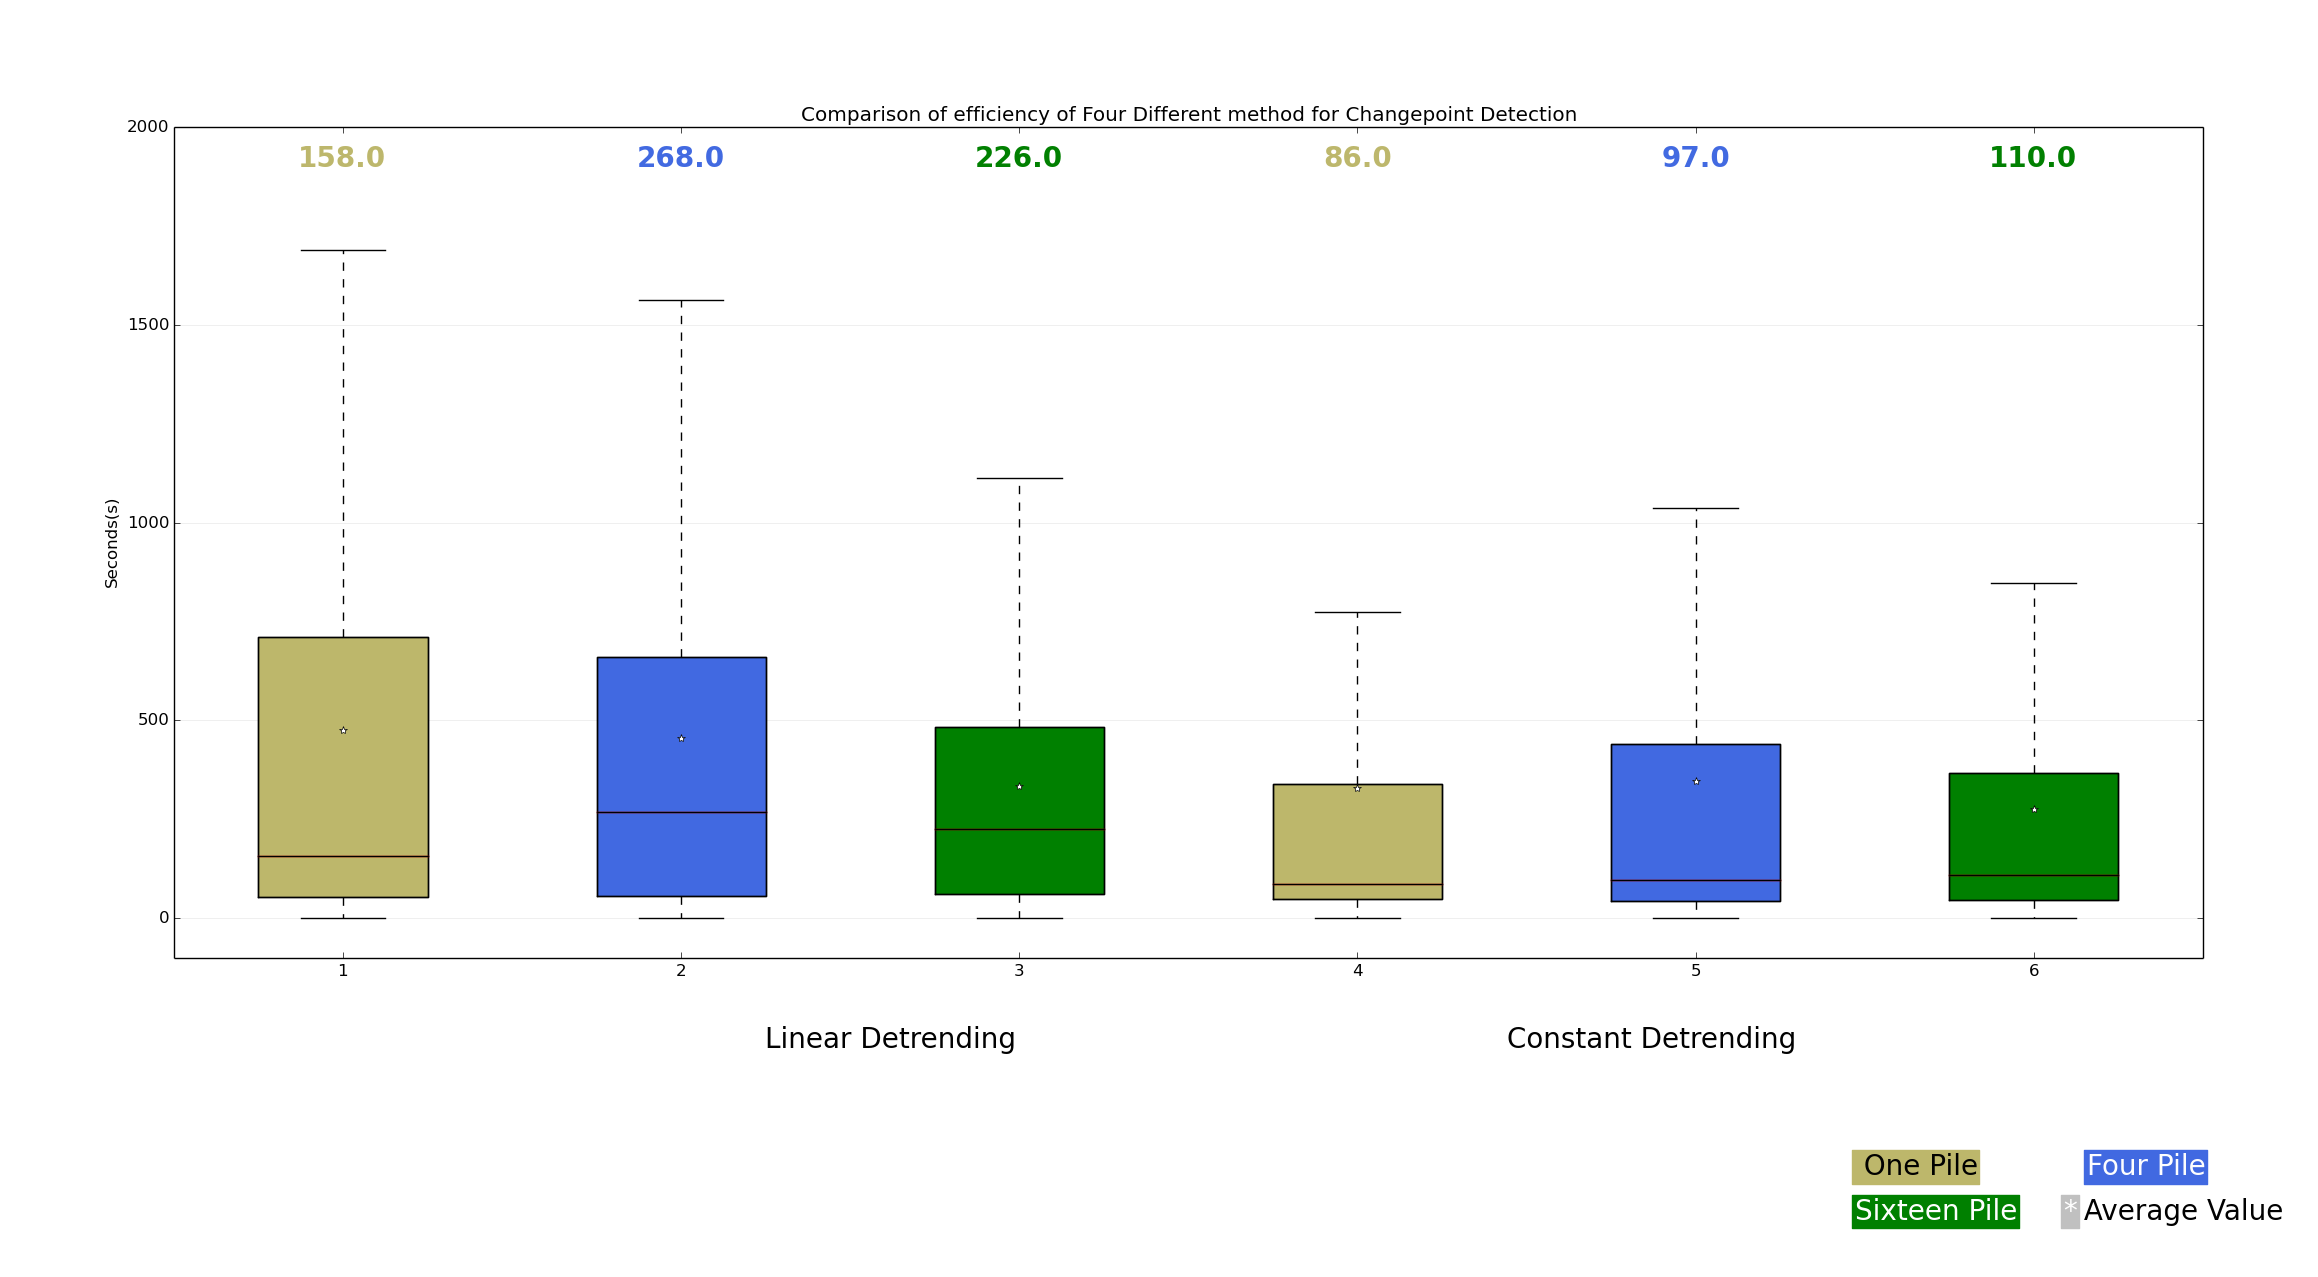
\includegraphics[width=\textwidth,height=0.35\textheight]{SiteFidelityOnly/SiteFidelity_WithoutOutlier_2.png}
	\caption{Comparison of all methods without outliers on data of \textit{P. rugosus} for memory only parameters}
\end{figure}
\begin{figure}
	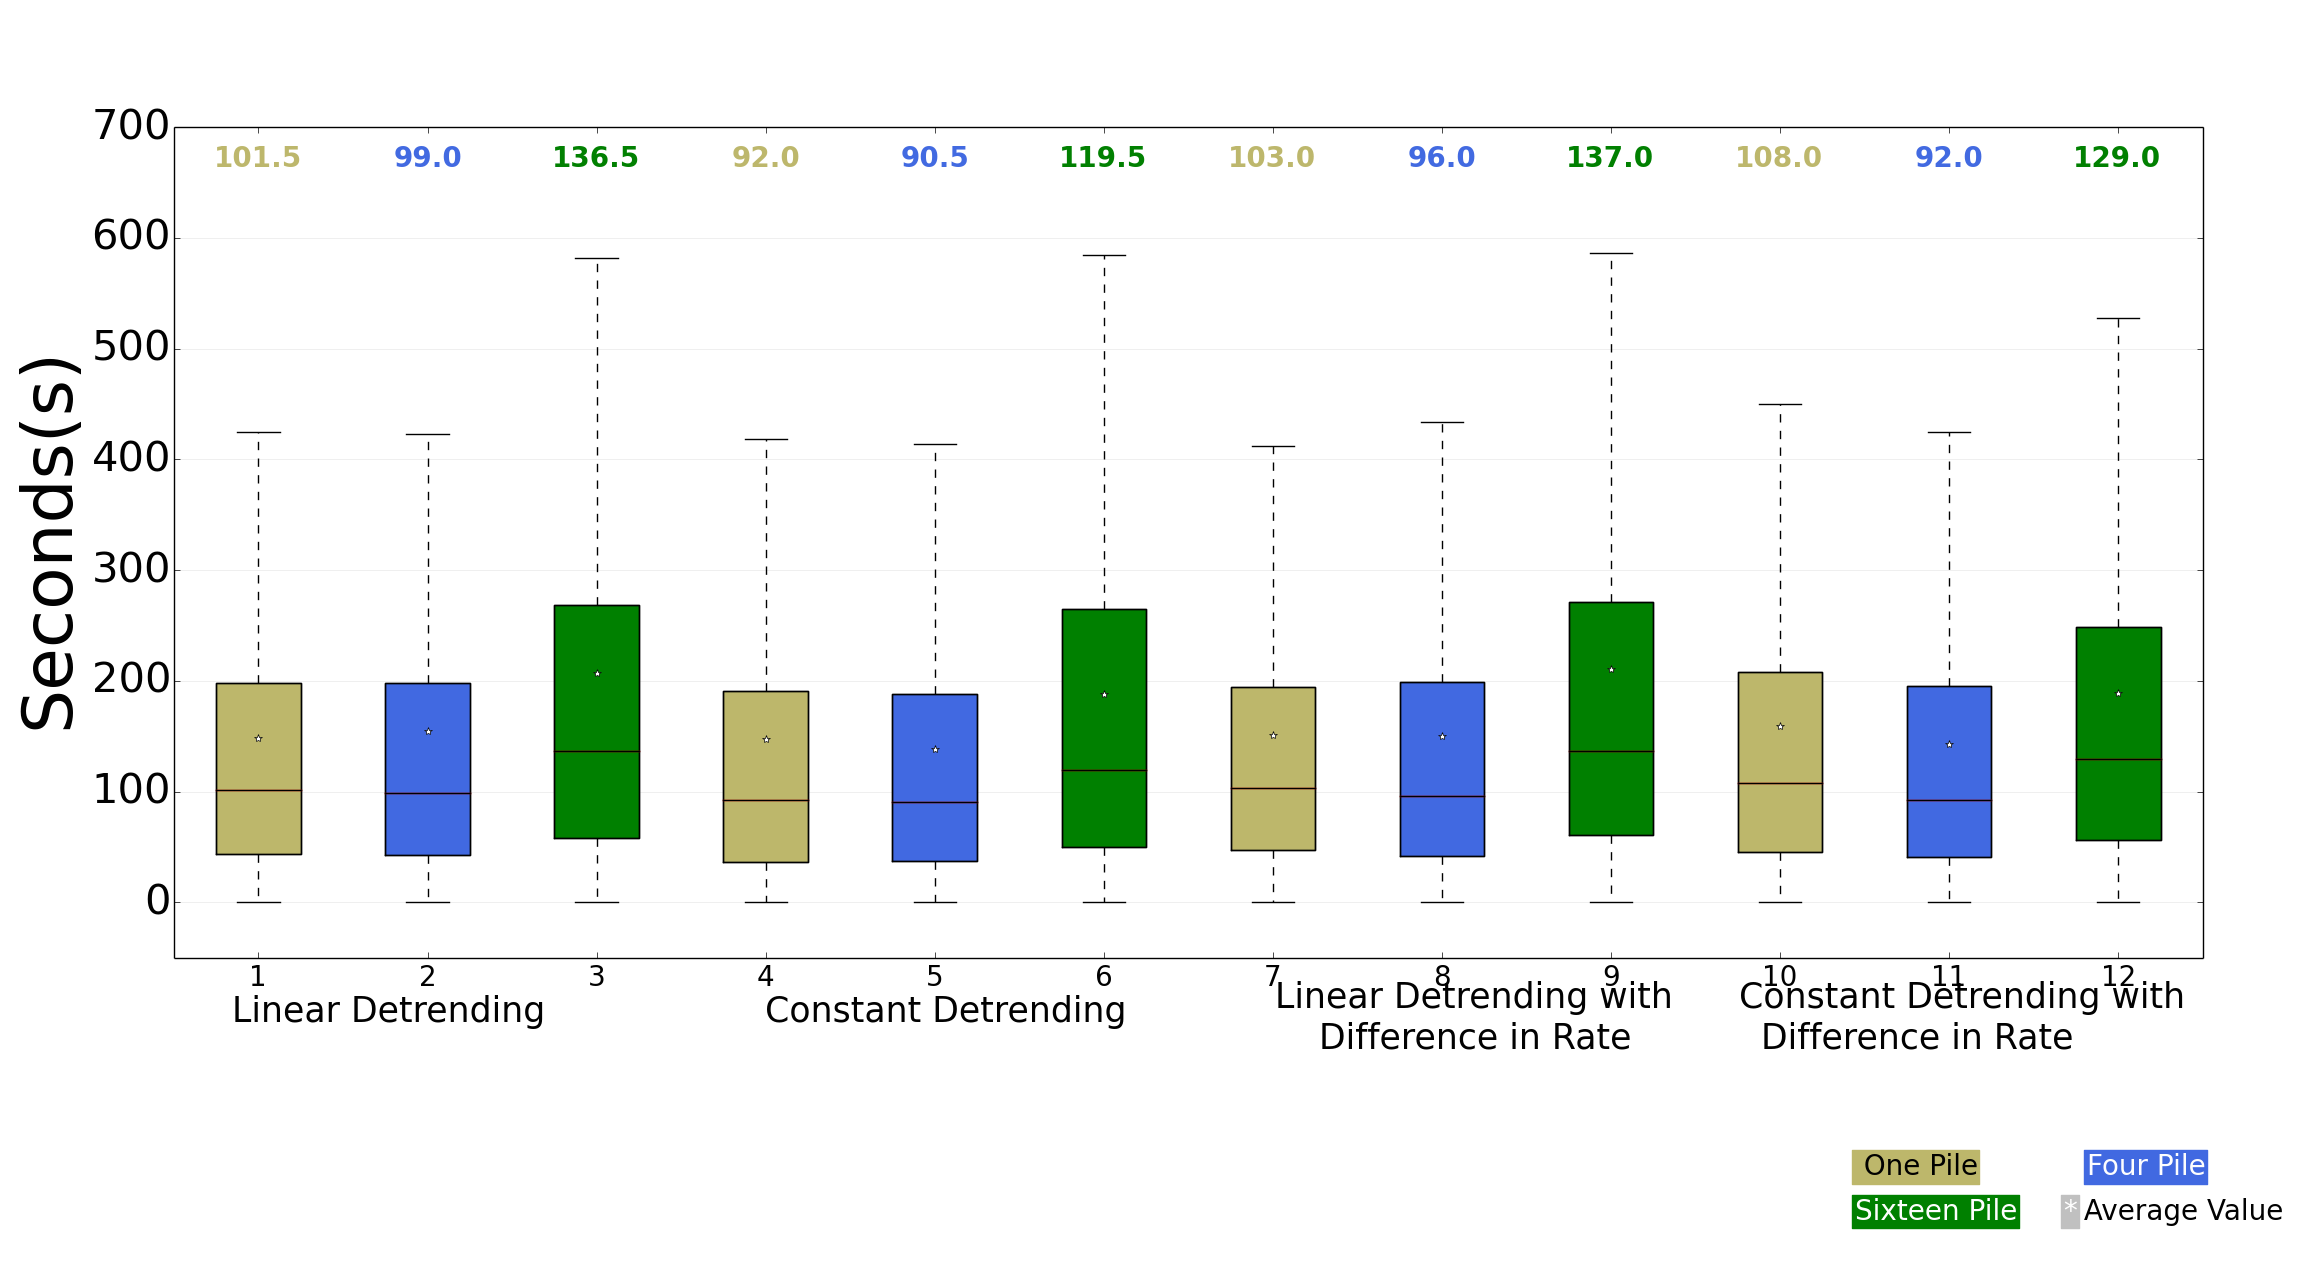
\includegraphics[width=\textwidth,height=0.35\textheight]{NewResult/All96.png}
	\caption{Efficiency of all methods with 96 ants for both combination of communication and memory}
\end{figure}
\begin{figure}
	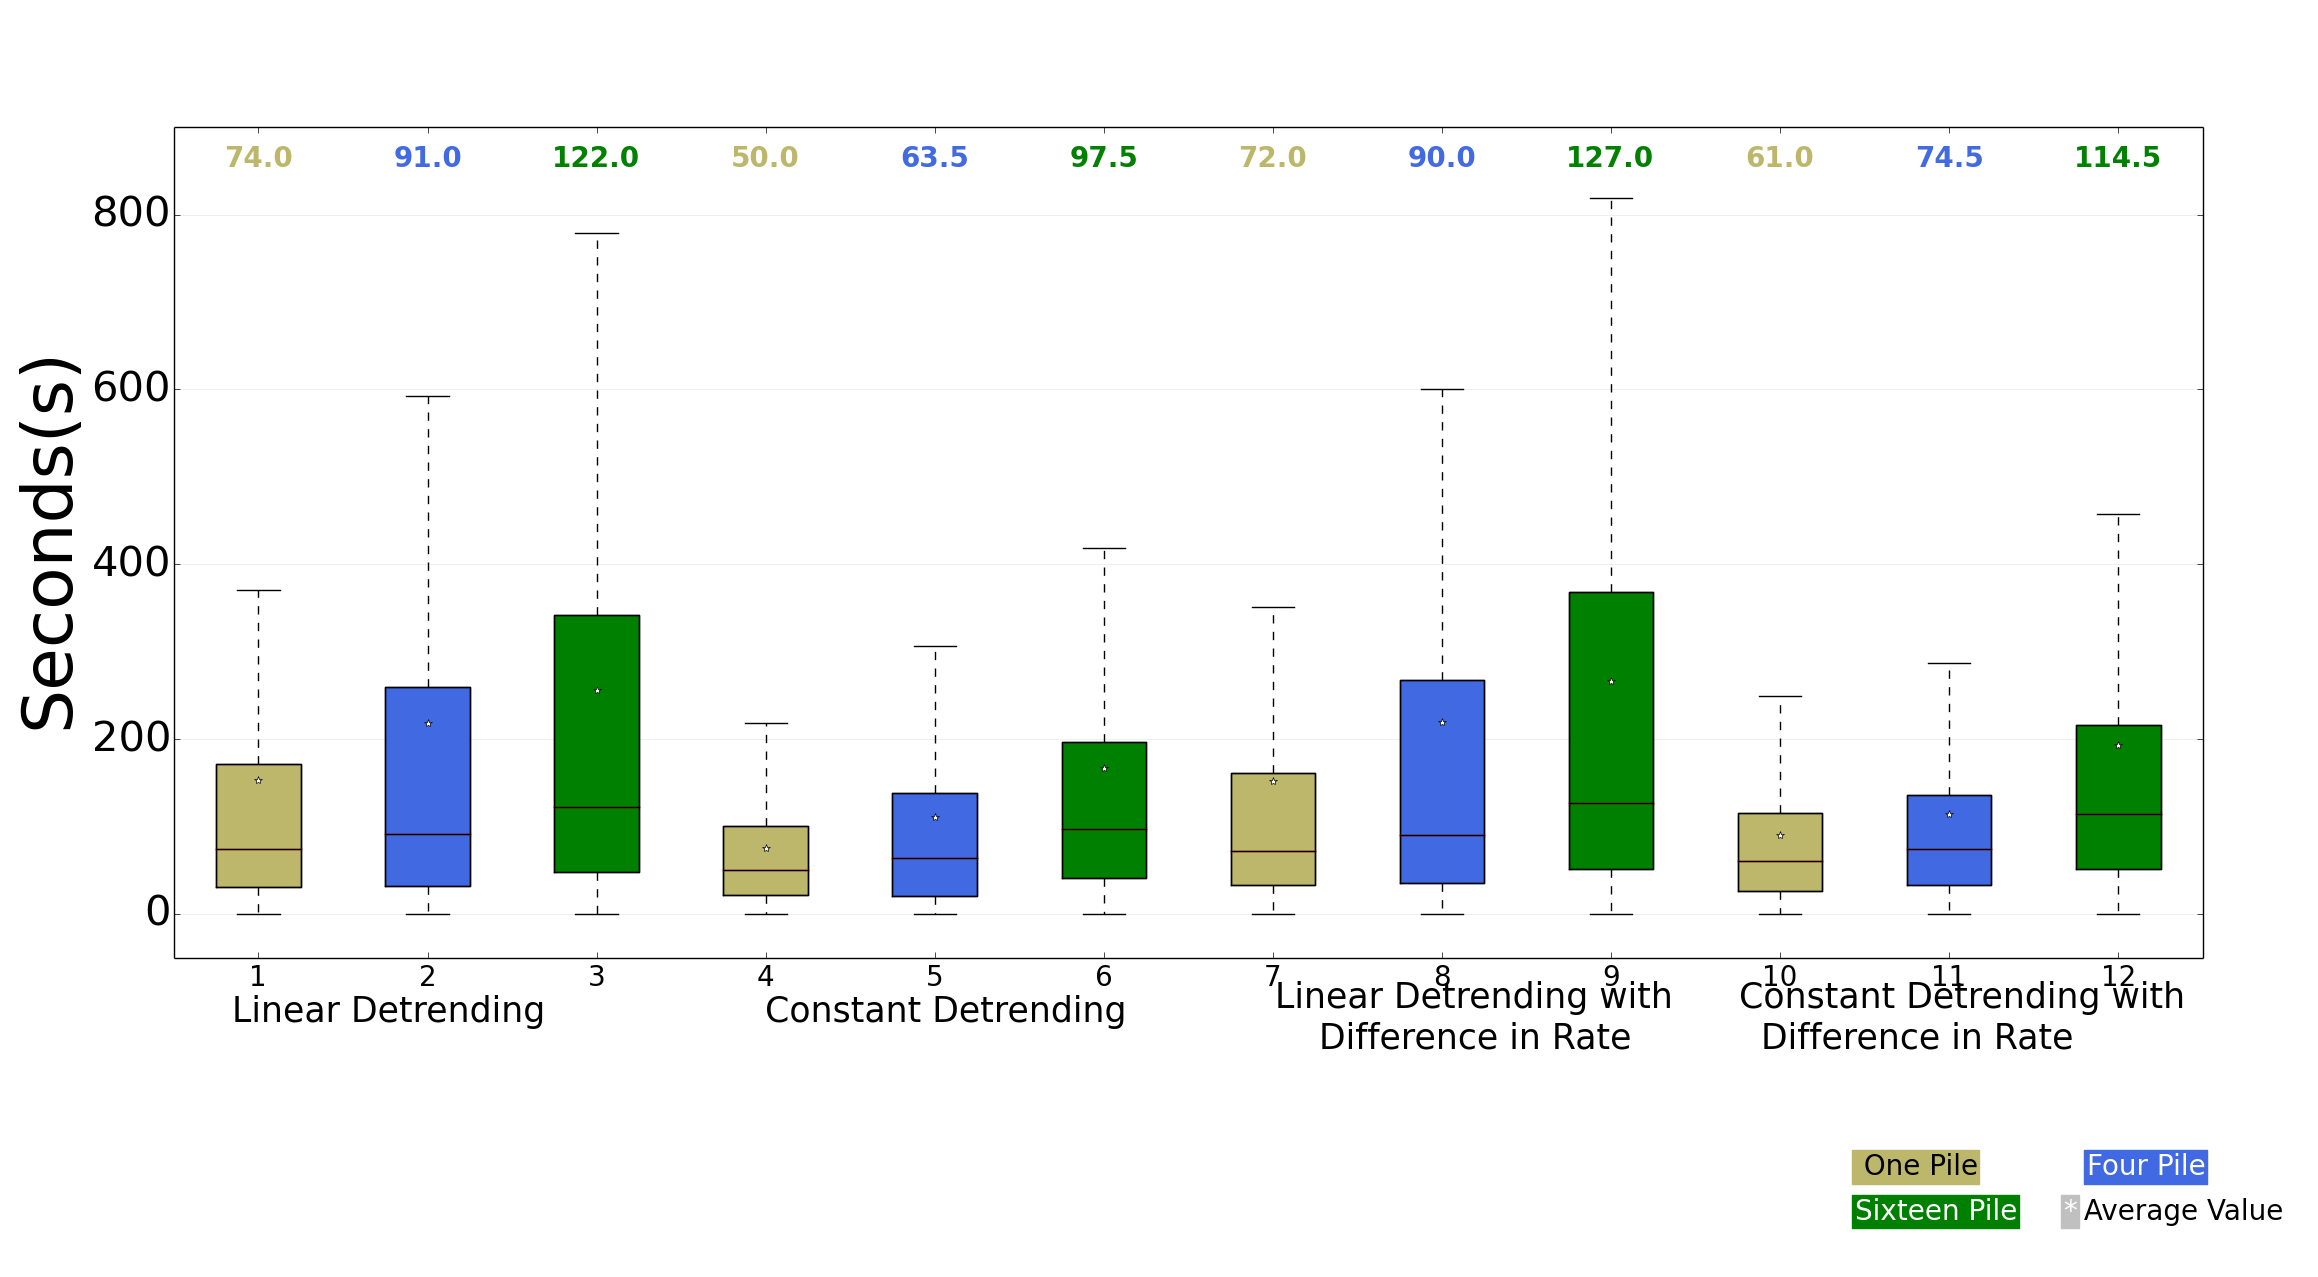
\includegraphics[width=\textwidth,height=0.35\textheight]{NewResult/All48.png}
	\caption{Efficiency of all methods with 48 ants for both combination of communication and memory}
\end{figure}
\clearpage
\begin{figure}[h]
	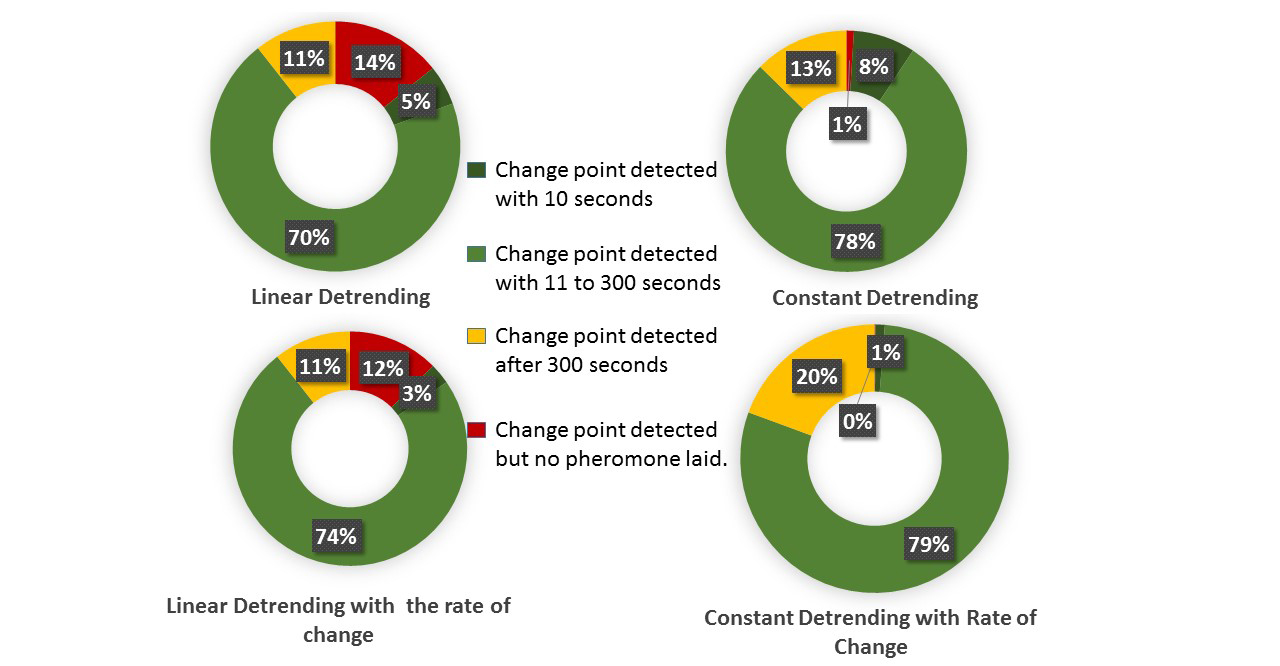
\includegraphics[width=\textwidth]{NewResult/Slide32.JPG}
	\caption{Efficiency chart for 96 ants, one pile,  memory and communication setting.}
\end{figure}
\begin{figure}[h]
	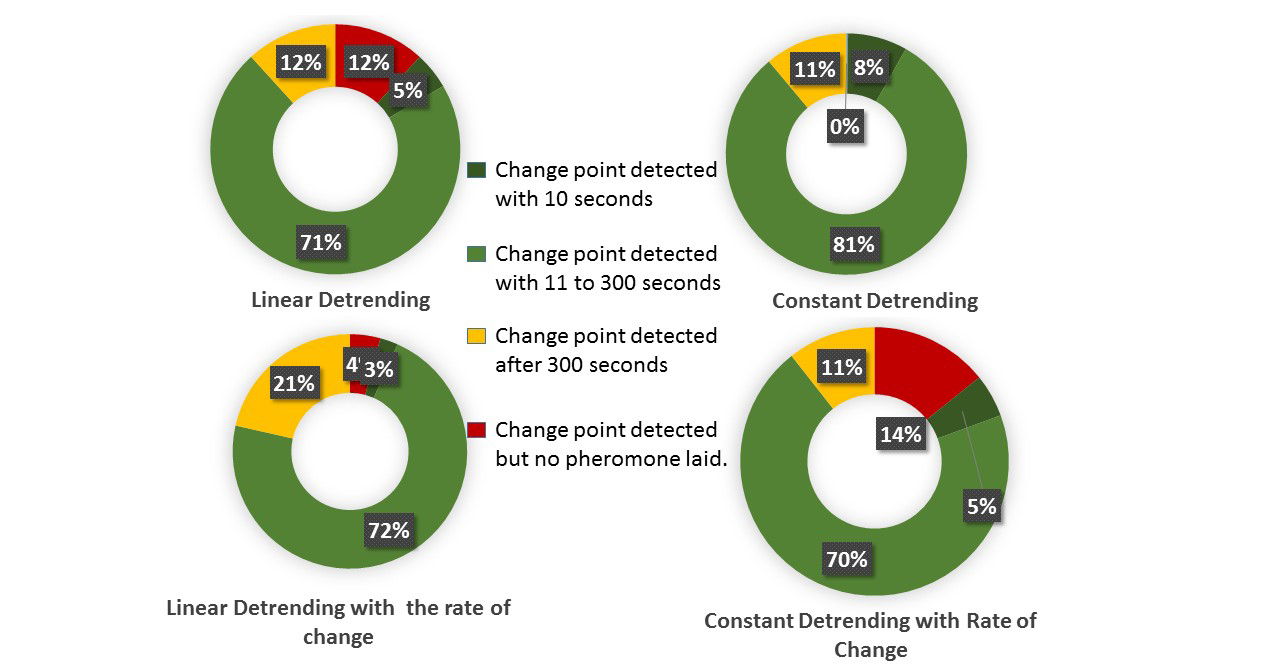
\includegraphics[width=\textwidth]{NewResult/Slide33.JPG}
	\caption{Efficiency chart for 96 ants, four pile,  memory and communication setting.}
\end{figure}

\begin{figure}[h]
	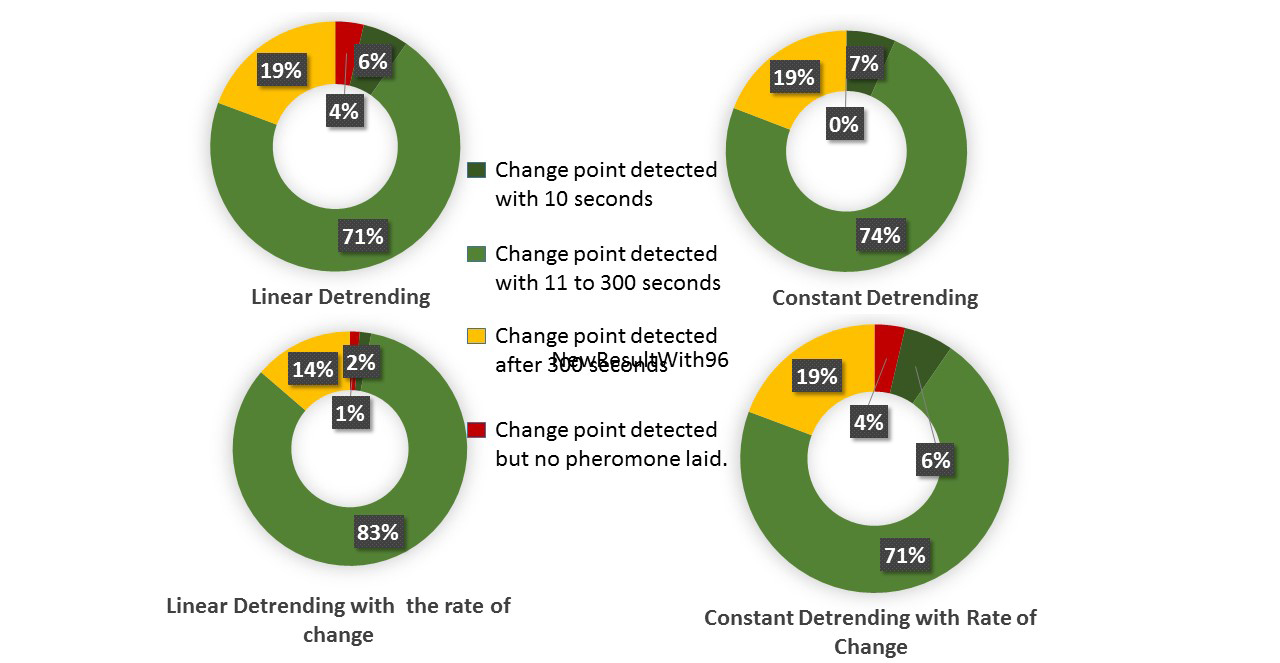
\includegraphics[width=\textwidth]{NewResult/Slide34.JPG}
	\caption{Efficiency chart for 96 ants, sixteen pile,  memory and communication setting.}
\end{figure}
\begin{figure}[h]
	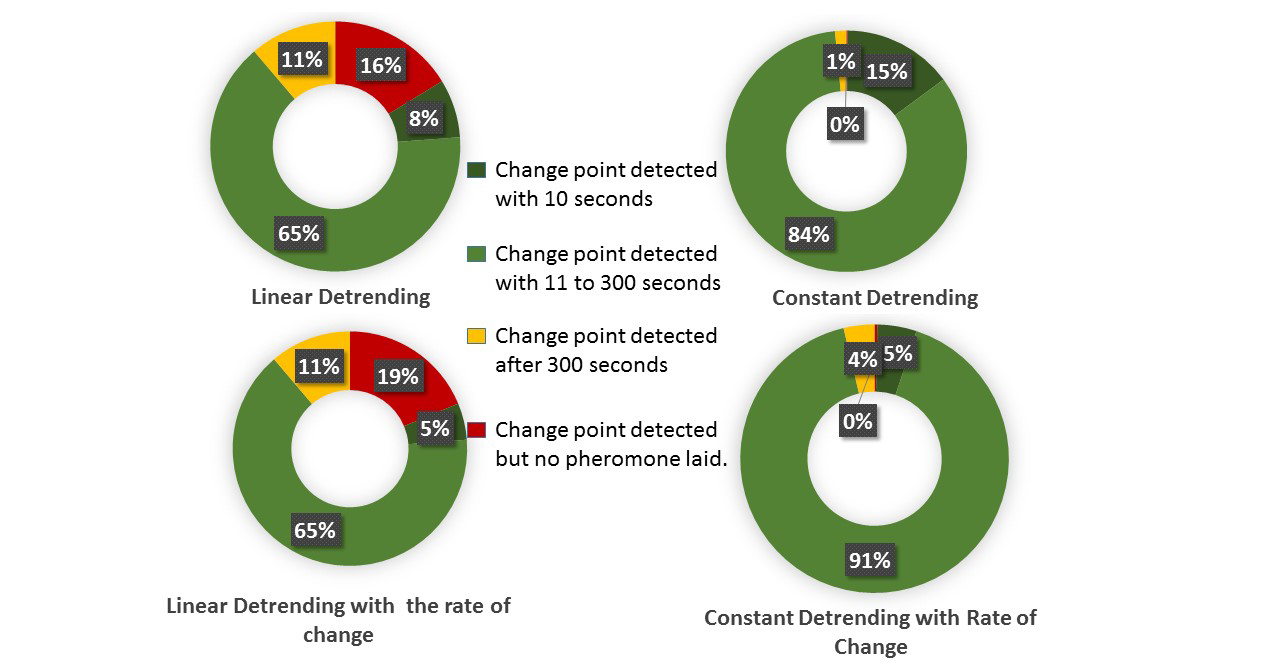
\includegraphics[width=\textwidth]{NewResult/Slide35.JPG}
	\caption{Efficiency chart for 48 ants, one pile,  memory and communication setting.}
\end{figure}
\begin{figure}[h]
	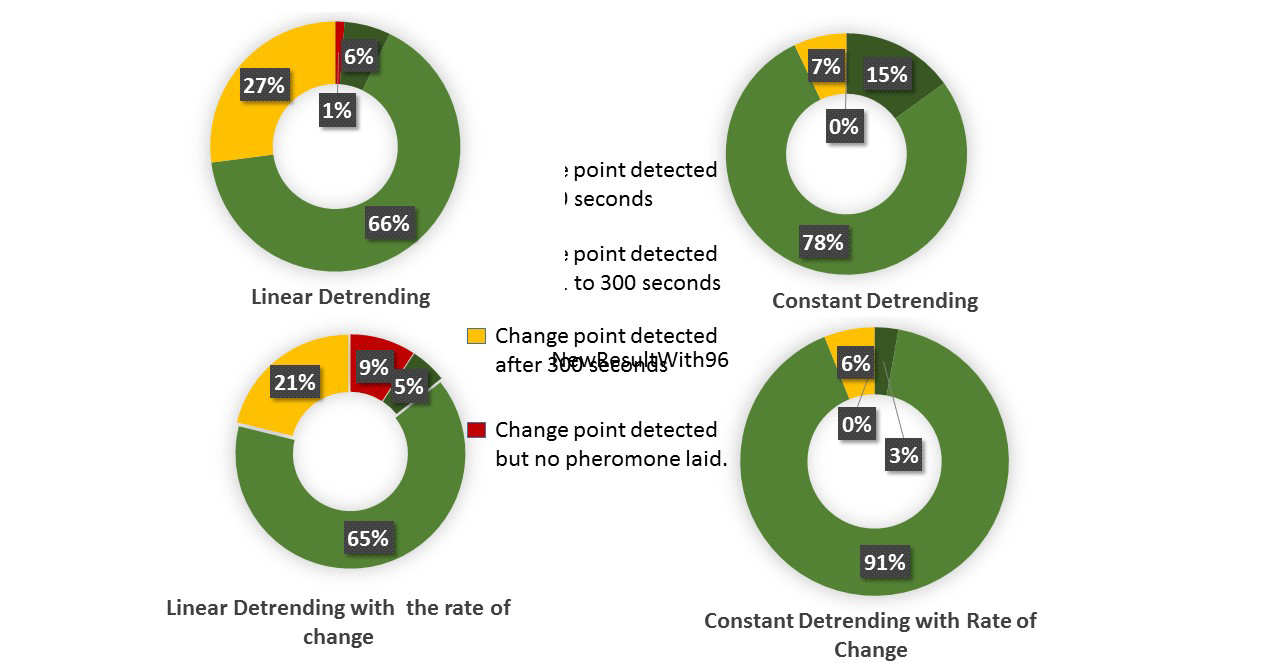
\includegraphics[width=\textwidth]{NewResult/Slide36.JPG}
	\caption{Efficiency chart for 48 ants, four pile,  memory and communication setting.}
\end{figure}
\begin{figure}
	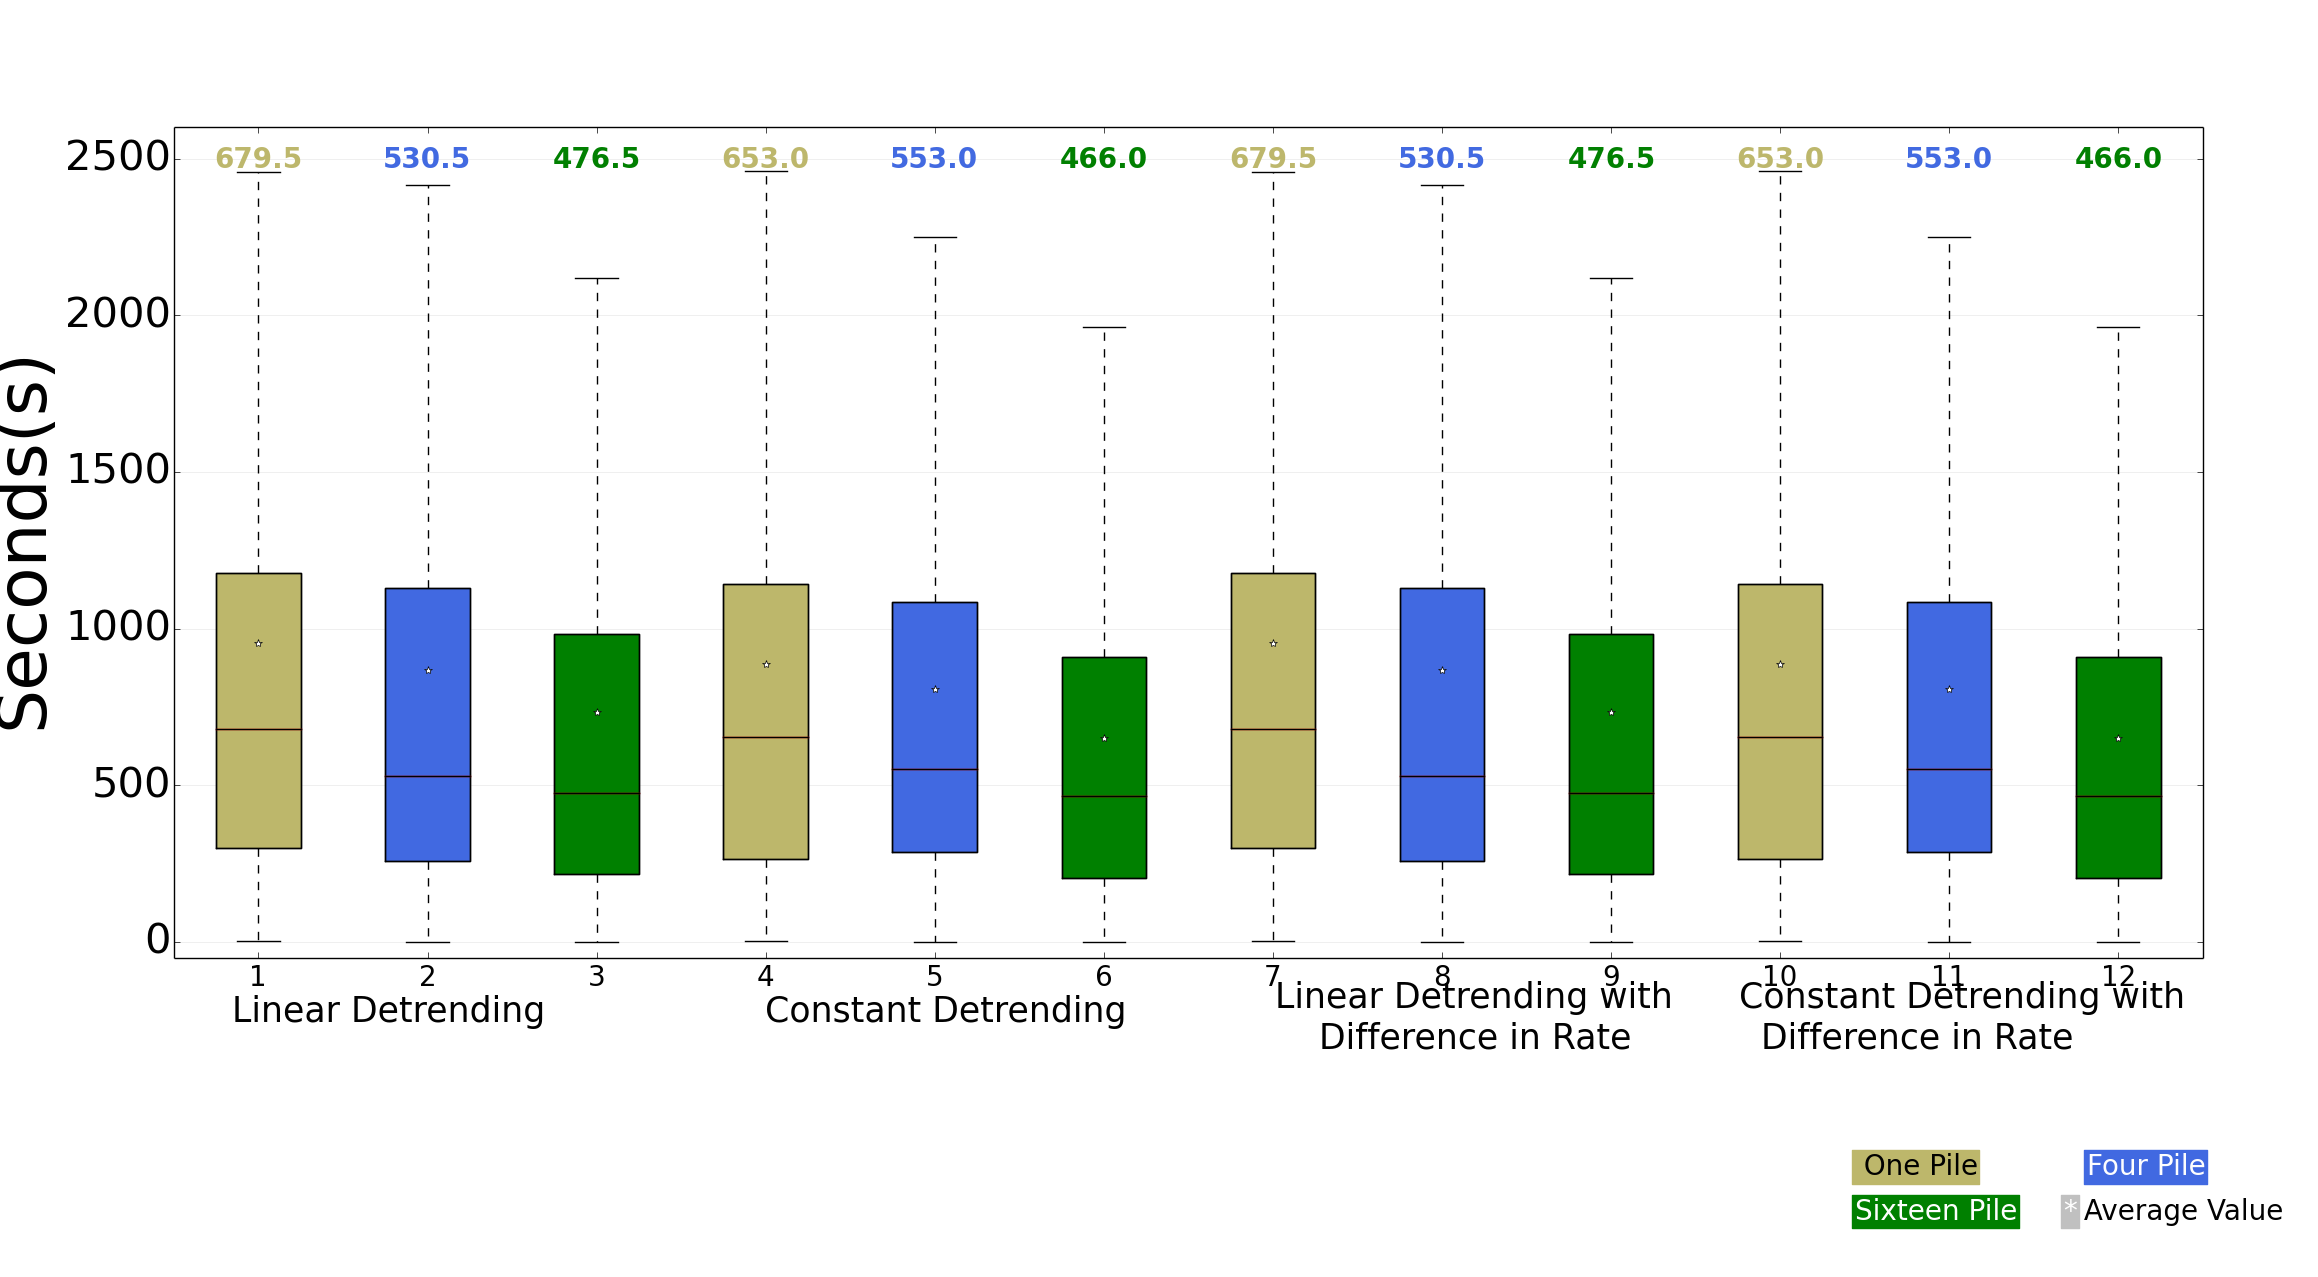
\includegraphics[width=\textwidth,height=0.35\textheight]{NewResult/SiteFidelity96.png}
	\caption{Efficiency of all methods with 96 ants for memory only parameters}
\end{figure}

\begin{figure}
	\includegraphics[width=\textwidth,height=0.35\textheight]{NewResult/Run48SiteFidelity.png}
	\caption{Efficiency of all methods with 48 ants for memory only parameters}
\end{figure}
\begin{figure}[h]
	\includegraphics[width=\textwidth]{NewResult/Slide38.JPG}
	\caption{Efficiency chart for simulation with 96 ants, one pile,  memory only setting.}
\end{figure}
\begin{figure}[h]
	\includegraphics[width=\textwidth]{NewResult/Slide39.JPG}
	\caption{Efficiency chart for simulation with 96 ants, four pile,  memory only setting.}
\end{figure}
\begin{figure}[h]
	\includegraphics[width=\textwidth]{NewResult/Slide40.JPG}
	\caption{Efficiency chart for simulation with 96 ants, sixteen pile,  memory only setting.}
\end{figure}
\begin{figure}[h]
	\includegraphics[width=\textwidth]{NewResult/Slide42.JPG}
	\caption{Efficiency chart for simulation with 48 ants, one pile,  memory only setting.}
\end{figure}
\begin{figure}[h]
	\includegraphics[width=\textwidth]{NewResult/Slide43.JPG}
	\caption{Efficiency chart for simulation with 48 ants, four pile,  memory only setting.}
\end{figure}
\begin{figure}[h]
	\includegraphics[width=\textwidth]{NewResult/Slide44.JPG}
	\caption{Efficiency chart for simulation with 48 ants, sixteen pile,  memory only setting.}
\end{figure}

\begin{figure}[h]
	\includegraphics[width=\textwidth]{DesertorumDonutCharts/Slide20.JPG}
	\caption{Efficiency chart for \textit{P. desertorum}, sixteen pile,  memory only setting.}
\end{figure}
\begin{figure}[h]
	\includegraphics[height=0.4\textheight,width=\textwidth]{AllParameters/RawFit/96AntsSFPH.PNG}
	\caption{Efficiency of change point detection algorithm on foraging rate and change in foraging rate for memory plus communication parameters.}
\end{figure}
\begin{figure}[h]
	\includegraphics[height=0.4\textheight,width=\textwidth]{SiteFidelityOnly/RawFit/96AntsSF.PNG}
	\caption{Efficiency of change point detection algorithm on foraging rate and change in foraging rate for memory only parameters.}
\end{figure}
\begin{figure}[h]
	\includegraphics[height=0.4\textheight,width=\linewidth]{NewResult/RandomSeed_43109511.png}
	\caption{A plot of seed collection from simulation of 96 ants.}
\end{figure}
\begin{figure}[h]
	\includegraphics[height=0.4\textheight,width=\linewidth]{NewResult/DP9.png}
	\caption{A plot of seed collection from one of the field experiment of \textit{P. desertorum} with change points on the collection rate.}
\end{figure}
